\documentclass[12pt]{article}

\usepackage[]{graphicx}
\usepackage[]{color}
\usepackage{alltt}
\usepackage{amsmath}
\usepackage{amssymb}
\usepackage{acronym}
\usepackage{multirow} 
\usepackage{float}
\usepackage{booktabs}
\usepackage{tikz}
\usetikzlibrary{positioning, arrows.meta, fit, calc, backgrounds}
\usepackage{pifont} % For checkmark symbol
\usepackage{titlesec}
\titlespacing*{\paragraph}{0pt}{0pt}{0.5em}

\usepackage[T1]{fontenc}
\usepackage{lmodern}
\usepackage[utf8]{inputenc}
\usepackage{textcomp}

\newcommand{\mytitle}{Self-Organization Patterns in LLM-based Multi-Agent Systems}
\newcommand{\myname}{Eric Echtermeyer}
\newcommand{\mysupervisor}{Prof. Dr. Hinrich Schütze, Ali Modarressi}
\newcommand{\suitename}{\textsc{soma}}
\newcommand{\arguephase}{\textit{Argue}}
\newcommand{\updatephase}{\textit{Update}}

\usepackage[a4paper, width = 160mm, top = 35mm, bottom = 30mm, 
bindingoffset = 0mm]{geometry}
\usepackage[utf8]{inputenc}
\usepackage{ragged2e}
\usepackage{xcolor}
\usepackage[round, comma]{natbib}
\usepackage{tabularx}
\usepackage{fancyhdr}
\newcommand{\changefont}{%
    \fontsize{8}{11}\selectfont
}
\usepackage{hyperref}
\hypersetup{
  colorlinks = true,
  linkcolor = black,
  urlcolor = black,
  citecolor = black}
\pagestyle{fancy}
\fancyhead{}
\fancyhead[R]{\changefont{\mytitle}}
\fancyfoot{}
\fancyfoot[R]{\thepage}
\setlength{\headheight}{14.5pt}
\setlength{\parindent}{0pt}
\setlength{\parskip}{0.8em plus 0.2em minus 0.1em}
\interfootnotelinepenalty = 10000

% Force et al. for entries with 5+ authors
\shortcites{du2024improving,chan2024chateval,liang2024encouraging,chen2024agentverse,
  chuang2025debate,achiam2023gpt4,liu2025stopovervaluing,wei2022chainofthought,
  rein2024gpqa,becker2025orchestration,ouyang2022instructgpt,li2024sparsetopology,
  liu2024groupdebate,miehling2025agentic,zhou2024sotopia,chang2024partnr,
  zhu2025multiagentbench,kenton2024debate,yang2025revisiting,zhang2024socialpsych,
  choi2025groupconformity,hendrycks2021mmlu,hendrycks2021math,wang2023selfconsistency,
  vaswani2017attention,zheng2023mtbench,zhu2026demystifying}

\renewcommand{\sectionautorefname}{Section}
\renewcommand{\subsectionautorefname}{Section}
\renewcommand{\subsubsectionautorefname}{Section}

% Custom float for verbatim prompt templates, to populate a List of Prompts
\newfloat{prompt}{H}{lop}
\floatname{prompt}{Prompt}
\newcommand{\promptautorefname}{Prompt}

% ------------------------------------------------------------------------------
% MAIN -------------------------------------------------------------------------
% ------------------------------------------------------------------------------
\IfFileExists{upquote.sty}{\usepackage{upquote}}{}


\begin{document}

% FRONT PAGE -------------------------------------------------------------------

\pagenumbering{Roman}

\begin{titlepage}
\begin{center}
    
\LARGE
Master Thesis
    
\vspace{0.5cm}
      
\rule{\textwidth}{1.5pt}
\LARGE
\textbf{\mytitle}
\rule{\textwidth}{1.5pt}
   
\vspace{0.5cm}
      
\large
Department of Statistics \\
Ludwig-Maximilians-Universität München 

\vfill

\Large
\textbf{\myname}

\vfill

\large
Munich, September 30\textsuperscript{th}, 2026
      
\vfill


\includegraphics[width = 0.4\textwidth]{sigillum.png}

\vfill

\normalsize

Supervised by \mysupervisor

\end{center}
\end{titlepage}

% CONTENTS ---------------------------------------------------------------------

\newpage

\begin{abstract}

Multi-agent debate, where several language model agents answer on their own and then
argue and revise over several rounds, is widely promoted as a way to make models
reason better together. It is judged almost entirely by outcome metrics, usually the
accuracy of the final answer, which record where a deliberation ended but nothing
about how it got there. The failures reported for debate are all about the how.
Groups lock onto what they already share instead of pooling what individual agents
privately know, and agents drop a correct answer rather than challenge a confident
peer. Two debates can end on the same answer, one because the group weighed the
arguments and one because it only amplified the position it began with, and an
outcome metric scores both alike. Explaining what that score is tracking means
measuring the trajectory, which is what the study of dynamical systems is for.

We treat cooperative LLM debate as such a system and define \suitename{}, four
detectors that read recurring patterns from ordinary debate logs, each tested against
a null model that destroys the pattern and leaves everything else intact. They track
confidence reinforcing whatever position an agent already holds, several stable
answers coexisting for the same question, influence concentrating on one agent, and
deliberation that oscillates instead of settling. We run them over $30{,}000$ debates
across a grid of communication topologies and memory windows, on GPQA-Diamond, where
agents usually start with the correct answer somewhere in the group, and HiddenBench,
where they start systematically wrong.

The four patterns turn out to be faces of one mechanism, and together they explain
what accuracy was tracking all along. Debate mostly amplifies the votes it starts
with rather than reasoning a new answer into existence. A seeding experiment that
fixes only the opening votes makes this causal, since adding one correct agent to an
otherwise wrong opening lifts accuracy from $1.8\,\%$ to $26.2\,\%$, while the group
almost never recovers an answer no agent initially held. Topology and memory window
change how fast a debate settles and how much influence concentrates, but not how
often it is right. What can be acted on is the opening composition, because diverse
starting positions make it far more likely that the group elects an informed leader,
and those runs are markedly more accurate.

Every detector runs on logs a system already produces, so each doubles as a candidate
health check on a live deliberation. All claims are bounded to the setting we tested,
a homogeneous, cooperative, four-agent debate on one model family.

\end{abstract}

\newpage
\tableofcontents

\newpage

% CHAPTERS ---------------------------------------------------------------------

\pagenumbering{arabic}
    
\section{Introduction}
\label{sec:introduction}
\subsection{Motivation}
\label{sec:intro:motivation}

Large language models (LLMs) are increasingly deployed not as isolated
predictors but as interacting agents that reason, argue, and decide in groups.
A prominent instance of this shift is \emph{multi-agent debate} (MAD), in which
several LLM instances independently propose answers, exchange their reasoning
over multiple rounds, and revise their positions before the group commits to a
final decision \citep{du2024improving}. Across factual and mathematical
reasoning tasks, this simple protocol has been reported to improve accuracy and
reduce hallucination relative to a single model answering alone
\citep{du2024improving, liang2024encouraging, chen2024reconcile}, and it now
underpins a growing family of collaborative and evaluative systems
\citep{chan2024chateval}. The appeal is intuitive: independent agents make
partially independent errors, and deliberation offers a mechanism for the group
to identify and correct them.

This optimistic reading, however, rests almost entirely on \emph{outcome}
measurements. The literature evaluates multi-agent systems predominantly by
final task performance, treating the deliberation itself as an opaque process
that either does or does not yield a better answer. Recent critical
reassessments show that this outcome-centric view is fragile: debate frequently
fails to outperform single-model baselines, collapses under controlled comparison
with simpler alternatives, and exhibits failure rates between 41\% and 86.7\%
across seven frameworks \citep{liu2025stopovervaluing, zhang2025debateorvote,
bertalanic2026costofconsensus, cemri2025mast}. More
troublingly, the failures that do occur are not random noise but exhibit
structure. When two LLMs debate, both tend to grow \emph{more} confident that
they have won as the exchange proceeds, with confidence escalating away from a
rational baseline even when no new supporting evidence is introduced
\citep{prasad2025certain}. Under distributed information, groups of LLM agents
converge prematurely on the evidence they already share and fail to surface the
private knowledge needed for the correct answer, so that collective accuracy
collapses far below what a single agent achieves with complete information
\citep{li2026hiddenbench}. Purely cooperative framings can further collapse the
debate into a mutually agreeing echo chamber, a failure mode termed
Degeneration-of-Thought \citep{liang2024encouraging}.

What these pathologies have in common is that they are \emph{dynamical}. Rising
confidence, premature lock-in, and conformity cascades are properties of how
positions evolve and influence one another across rounds, not of any single
agent's competence at a single point in time. An outcome metric, by
construction, cannot see them: two systems can reach the same final accuracy
through entirely different trajectories, one through genuine error correction
and the other through a confident slide into a shared mistake. Understanding
\emph{when} and \emph{why} multi-agent deliberation succeeds therefore requires
a vocabulary for the interaction dynamics themselves. \citet{miehling2025agentic}
make precisely this argument at a conceptual level, contending that agentic AI
must be studied through a systems-theoretic lens because emergent group-level
behaviour cannot be predicted from individual agent properties alone. Their
position, however, remains programmatic and offers no empirical instrument for
detecting such behaviour in practice.

Complex-systems theory supplies exactly such an instrument. Systems of many
interacting units that produce ordered collective behaviour without central
control, the defining feature of self-organization \citep{ashby1947principles},
are known to fall into a small number of recurring dynamical regimes. These
regimes have precise names and precise signatures: \emph{self-reinforcement},
the positive feedback by which a state amplifies its own persistence
\citep{arthur1989competing}; \emph{limit cycles}, self-sustained periodic
oscillations that never settle \citep{strogatz2015nonlinear};
\emph{bistability}, the coexistence of multiple stable outcomes selected by
initial conditions \citep{feudel2008complex}; and \emph{dominance}, the
concentration of influence onto a single node \citep{degroot1974consensus,
jia2015opinion}. Such patterns are studied as \emph{motifs}, recurring structural or
dynamical building blocks whose presence in a system is both detectable and
diagnostic of its behaviour \citep{milo2002network, alon2007network,
driscoll2024dynamical}. The pathologies documented in the MAD literature read
naturally as instances of this vocabulary: escalating confidence is a
self-reinforcement signature, premature consensus is a fixed-point attractor
reached through basin selection, and herding to a confident leader is a
dominance motif. The connection has begun to be made.
\citet{ashery2025conventions} demonstrate the spontaneous emergence of
universally adopted social conventions in decentralised LLM populations, show
that strong collective biases arise even when individual agents exhibit none,
and find that committed adversarial minorities can impose alternative
conventions on the majority. \citet{okawa2026biasedconsensus} derive a formal model predicting that once
conformity pressure among agents exceeds a critical threshold, the group is
pulled toward a shared bias regardless of what any individual agent believes.
What these treatments share is a substrate in which no option is better than any
other, so they can show that a group locks in but not whether it locks in on the
right answer; \citet{mehdizadeh2026topologymemory} name the epistemic case, where
some claims are better supported than others, as a critical open question.

This thesis addresses that gap. We construct a controlled cooperative
multi-agent debate system in which homogeneous LLM agents deliberate over
multiple rounds on tasks with verifiable ground truth, and we develop a suite of
detectors, each grounded in the complex-systems and opinion-dynamics literature,
that identify self-reinforcement, limit cycles, bistability, and dominance in
the resulting interaction logs. We run this system across a controlled grid of
communication topologies and memory configurations on two complementary
benchmarks: GPQA-Diamond \citep{rein2024gpqa}, a graduate-level science
question-answering benchmark where agents typically start with reasonable priors,
and HiddenBench \citep{li2026hiddenbench}, a hidden-profile benchmark
constructed so that agents start systematically wrong and success requires
genuine information pooling. The contrast between the two isolates whether
observed dynamics depend on the presence of a reliable individual signal or
persist even when the group must correct a shared bias. Throughout, we treat
motif detection not as a competitor to accuracy but as an explanatory layer
beneath it: a way to characterise the trajectory that produces an outcome, and
thereby to understand which design choices shape the deliberative dynamics of
LLM collectives.

This explanatory layer has a practical purpose. As multi-agent systems are
deployed in consequential settings, an operator needs to know not only whether a
configuration tends to produce correct answers but whether a given deliberation
is proceeding soundly or pathologically, whether the group is genuinely
correcting an error or confidently converging on a shared mistake, and whether it
will terminate at all. Outcome metrics cannot answer these questions.
Instruments are beginning to appear from other directions: online monitors
based on conditional transfer entropy over execution traces
\citep{caspian2026} and learned classifiers that predict from interpretable
features whether a query warrants debate at all \citep{fan2026imad}. What does
not yet exist is an instrument grounded in the dynamical vocabulary itself, one
that names which regime a deliberation is in rather than only flagging that
something is wrong. A
central thread of this thesis is therefore that each motif detector, being
computed from ordinary interaction logs, doubles as a candidate \emph{diagnostic}
of deliberative health. We do not deliver a validated diagnostic tool; we deliver
the empirical groundwork for one, a set of measurable signatures, characterised
across a controlled grid, together with tiered, evidence-graded design principles
that state honestly how far each is supported by our data.

In one sentence, the objective of this thesis is to understand \emph{how} a
cooperative LLM debate arrives at its answer, by measuring the self-organization
patterns in its trajectory, and to turn that understanding into evidence-graded
guidance for building such systems.


\subsection{Research Questions}
\label{sec:intro:rqs}

The overarching goal of this thesis is to establish whether the dynamical
vocabulary of complex systems can be applied empirically to LLM-based
multi-agent debate, and to characterise the conditions under which
self-organization patterns emerge. We decompose this goal into three research
questions, ordered by the class of evidence each requires.

\begin{itemize}
  \item[\textbf{RQ1}] \textbf{Measurement.} Can self-organization motifs,
        specifically self-reinforcement, limit cycles, bistability, and
        dominance, be detected in cooperative LLM-based multi-agent debate using
        detectors grounded in the complex-systems and opinion-dynamics literature
        and each tested against a principled null model? And which of these motifs
        actually occur, at what prevalence, and with what structure?

  \item[\textbf{RQ2}] \textbf{Characterisation.} What governs the presence and
        strength of each motif, and what do they predict about system outcomes?
        We examine the two canonical structural axes, communication topology and
        memory window, together with the information regime of the task and the
        composition of the opening votes, and ask what each motif implies for
        accuracy, convergence speed, and worst-case runtime.

  \item[\textbf{RQ3}] \textbf{Causation.} Is the composition of the opening votes
        causally responsible for the outcome? Can the system generate a correct
        answer that no agent initially held, or does deliberation function
        primarily as an amplifier of the initial vote distribution?
\end{itemize}

One commitment underpins these questions. Every detector is tested against a null model that destroys the pattern we look for and leaves everything else intact. This matters because our state space is small: with four agents and three or four options, votes repeat and influence concentrates by chance alone. The null tells us what chance looks like, so a near-zero prevalence becomes a measurement rather than a failure. We report the motifs we do not find alongside those we do.


\subsection{Contributions \& Structure}
\label{sec:intro:contributions}

This thesis makes three contributions, one for each research question.

\begin{itemize}
  \item \textbf{An instrument for measuring debate dynamics.} We define a
        two-phase synchronous debate protocol that separates public messages
        from private beliefs and confidences, so that the interaction log
        exposes exactly the quantities motif detection requires
        (\autoref{sec:exp}). On top of it we specify \suitename{}
        (Self-Organization Motif Analysis): detectors for self-reinforcement,
        bistability, dominance, and limit cycles, each grounded in the
        complex-systems or opinion-dynamics literature and each tested against
        its own null model (\autoref{sec:method}). Every detector states what it
        can and cannot claim, distinguishing a measured signature from a
        certified attractor. Running $R = 50$ repetitions of every task--config
        cell is what makes across-repetition attractor statistics measurable at
        all.

  \item \textbf{An empirical characterisation at scale.} We apply \suitename{}
        to 30{,}000 debates across twelve configurations and two deliberately
        contrasting benchmarks: a refinement regime in which agents mostly start
        correct, and a correction regime in which they start systematically
        wrong (\autoref{sec:results}). Self-reinforcement is universal and drives
        convergence, bistability is common and is a stable property of the task
        rather than of the configuration, dominance emerges behaviourally even
        under a symmetric topology, and genuine limit cycles are essentially
        absent outside the star, where they arise through a hub-driven
        mechanism. Reading the emergent influence graph within fully-connected
        runs reveals a lever the structural topology parameter cannot reach: a
        rare effective star, formed preferentially from diverse opening
        positions, is markedly more accurate than the fully-connected mean.
        Throughout, the structural axes we varied move the dynamics but not the
        accuracy.

    \item \textbf{A causal test of the initial-condition effect.} A
        seeded-initialisation experiment manipulates only the composition of the
        opening votes, leaving the debate itself unchanged. Inserting a single
        correct agent into an otherwise-incorrect opening raises accuracy from
        $1.8\,\%$ to $23.7\,\%$, and does so in all 34 tasks tested. In the
        unseeded arm, where no agent starts correct, the system arrives at the
        correct answer in under $2\,\%$ of repetitions, and its ability to do so
        declines as tasks get harder. A devil's advocate probe confirms the
        complementary vulnerability under a controlled composition: a single
        agent that never updates its position outweighs two agents that start
        correct, collapsing accuracy from $63.7\,\%$ to $10.0\,\%$. Together
        these upgrade the central claim from association to intervention: within
        the setting we tested, deliberation functions predominantly as a
        selective amplifier of its opening vote distribution
        (\autoref{sec:results}).
\end{itemize}

\noindent From these results we derive design guidance graded by how strongly our
data support each claim, and show that every \suitename{} detector, computed from
ordinary interaction logs, is a candidate observable for monitoring deliberative
health (\autoref{sec:discussion}). We deliver the measurements and the mapping
from principle to observable, not a packaged tool.

\paragraph{Structure of this thesis.}
The thesis follows the arc of the three research questions. \emph{Background}
(\autoref{sec:infsub}) introduces the vocabulary of self-organization and
dynamical motifs and fixes what we mean by an LLM agent and a debate;
\emph{Related Work} (\autoref{sec:related}) surveys how multi-agent systems are
currently analysed and locates the gap this thesis addresses. The instrument is
then built in two steps: \emph{System and Experimental Setup}
(\autoref{sec:exp}) specifies the debate protocol, the two contrasting
benchmarks, and the experimental grid, and \emph{Detection Methodology}
(\autoref{sec:method}) defines the four \suitename{} detectors together with the
null model each is tested against. \emph{Results} (\autoref{sec:results}) applies
the instrument, reporting accuracy and efficiency, the four motifs in turn, the
emergent influence topology, and the seeded-initialisation experiment.
\emph{Discussion} (\autoref{sec:discussion}) reads the motifs together as one
amplifier mechanism and distils the findings into evidence-graded design
principles. \emph{Limitations and Future Work} (\autoref{sec:limitations}) states
the scope of the claims and the agenda they imply, and
\emph{Conclusion} (\autoref{sec:conclusion}) returns to the three research
questions.
\newpage

\section{Background}
\label{sec:infsub}
% ============================================================
% CHAPTER 2: BACKGROUND
% All citations in this chapter reuse entries already present in
% bibliography.bib and verified during the Chapter 3 literature
% review. No new references are introduced here.
% ============================================================

Multi-agent debate is a multi-agent system, and its documented failures are
dynamical: they are properties of how positions evolve and influence one another
across rounds, not of any single agent's competence at a single moment. Naming
those failures precisely, and measuring them, requires a vocabulary for
dynamical systems. Most readers of this thesis are practitioners who know what
an LLM agent is and what multi-agent debate does; they are far less likely to
know what an attractor is, what a basin of attraction selects, or how influence
concentrates in a network through purely structural means. This chapter
therefore spends most of its space on the unfamiliar ground.
\autoref{sec:bg:complex} introduces complex systems and self-organization from
first principles: emergence, attractors, bistability, and positive feedback.
\autoref{sec:bg:motifs} casts those ideas as formal motifs and introduces
opinion dynamics, the branch of complex-systems theory that studies how
influence propagates and concentrates among interacting agents, and which
provides the closest formal model of what debate agents do.
\autoref{sec:bg:mad} fixes the familiar parts: what an LLM agent means in the
sense used here, how multi-agent debate works, and which failure modes motivate
this study. Formal definitions of the four detectors are deferred to
\autoref{sec:method}; the present chapter only establishes the ideas they rest
on.

% ============================================================
\subsection{Complex Systems and Self-Organization}
\label{sec:bg:complex}
% ============================================================

A \emph{complex system} is a collection of many interacting components that
collectively exhibit behaviour which cannot be read off from any individual
component in isolation. The behaviour is called \emph{emergent}: it is a
property of the interaction structure, not of any single unit. When such
emergent behaviour is ordered and coordinated and arises without any central
authority imposing it, the system is called \emph{self-organizing}
\citep{ashby1947principles}. No component decides the global outcome, yet a
global outcome reliably appears. A flock of birds, a developing embryo, and a
financial market are all self-organizing: each component follows local rules
about its immediate neighbours, yet the collective as a whole exhibits
coherent global structure that no individual plans or directs.

The natural language for self-organizing systems is that of dynamical systems
theory. The state of a system at a given moment is a point in a space whose
dimensions correspond to all quantities that describe the system; as time
passes, the system traces a \emph{trajectory} through that space. Not all
parts of the space are equally visited: over time, trajectories tend to settle
onto sets called \emph{attractors} \citep{strogatz2015nonlinear}. A
\emph{fixed-point attractor} is a state the system reaches and stays in: a
consensus, a locked configuration. A \emph{limit cycle} is a closed orbit the
system revisits indefinitely without settling, a permanent oscillation in which
the same sequence of states repeats in a regular cycle. The region of initial
conditions that eventually leads to a given attractor is its \emph{basin of
attraction}. Two initial conditions in the same basin converge to the same
long-run behaviour; two initial conditions in different basins do not.

A system is \emph{bistable} (or more generally \emph{multistable}) if two or
more distinct attractors coexist for the same parameter values
\citep{feudel2008complex}. Which attractor is reached is then determined
entirely by the initial condition: two runs of the same system with different
starting points can land on different long-run outcomes for purely dynamical
reasons, not because anything about the system itself changed. The boundary
between basins, the \emph{separatrix}, need not lie at an obvious midpoint. In
social systems, the corresponding phenomenon is a tipping point: a critical
minority is sufficient to move the collective from one stable state to another,
well below the majority that naive equilibrium reasoning would require.
\citet{centola2018tipping} establish experimentally that this critical mass is
roughly 25\% of the population, that it is robust across norm types, and that
longer interaction memories raise the threshold.

Two further regimes are central to this thesis. \emph{Self-reinforcement}, or
positive feedback, is the tendency of a state to amplify its own persistence:
an early lead grows because it is a lead, independently of whether it is
intrinsically superior. The canonical example is technology lock-in through
increasing returns, where a product's market share generates adoption that
further increases that share \citep{arthur1989competing}. Positive feedback
does not select the best option; it selects the option that accumulated an
early advantage. The complementary phenomenon is the \emph{concentration of
influence} onto a single component. In a network of interacting agents, one
node may come to disproportionately determine the collective state, not because
it is better informed, but because the interaction structure channels influence
through it. Both regimes, positive feedback and influence concentration, are
detectable from ordinary time-series records of the system's state, which is
why they admit an empirical instrument.

% ============================================================
\subsection{Dynamical Motifs and Opinion Dynamics}
\label{sec:bg:motifs}
% ============================================================

The patterns described above can be made precise as \emph{motifs}: recurring,
detectable signatures of a system's organization. The term carries two
complementary meanings that this thesis uses carefully. A \textbf{structural
motif} \citep{milo2002network, alon2007network} is a recurring pattern in the
\emph{wiring}: a small subgraph of who-connects-to-whom that appears in a
network more often than chance and generates characteristic input--output
behaviour. The archetypal example is the feed-forward loop, a three-node
circuit whose sign configuration makes it a sign detector or a pulse filter.
A \textbf{dynamical motif} \citep{driscoll2024dynamical} is instead a
recurring pattern in the \emph{trajectory}: an attractor, a periodic orbit, a
separatrix between basins of attraction. It is a statement about how the
system behaves over time rather than how it is wired. The two are linked,
since structural motifs are studied precisely because each generates a
characteristic dynamical regime, and they map onto the two levels at which
phenomena live in this thesis, the agent level and the system level.

This thesis detects four motifs, each selected because it has a precise,
testable signature and corresponds to a documented failure mode of multi-agent
debate. \emph{Self-reinforcement} is positive feedback at the agent level: an
agent that holds a position through a round emerges with higher rather than
lower confidence, a positive-autoregulation structural motif whose dynamical
signature is a rising confidence slope within vote-stable runs.
\emph{Limit cycles} are self-sustained periodic oscillations: a vote sequence
that revisits the same states in a repeating order without converging, a
dynamical motif readable from the discrete vote channel.
\emph{Bistability} is the coexistence of multiple stable consensus outcomes
across repetitions of the same task, a dynamical motif whose signature is a
multimodal outcome distribution that persists as the initial vote composition
varies. \emph{Dominance} is the concentration of causal influence onto a
single agent, reflected in a heavy-tailed distribution over an emergent
influence graph, a structural motif in the influence network that the debate
generates. Together the four span both senses of motif and both levels of
description.

The propagation and concentration of influence that underlie self-reinforcement
and dominance have a formal home in \emph{opinion dynamics}, which studies how
agreement and social power evolve in a network of interacting agents. The
classical model due to \citet{degroot1974consensus} treats each agent's
opinion as a weighted average of its neighbours' opinions at the previous step.
Under mild connectivity conditions this process reaches consensus: all agents
converge to the same value, which is a weighted combination of their initial
opinions. The coefficients in this combination are called \emph{social power}
\citep{jia2015opinion}, and they are not generally equal: an agent that is
upstream of many others accumulates disproportionate weight in the final belief,
even if its initial opinion is no more accurate than its peers'. This is the
formal analogue of the dominance motif: influence concentration arising from
network position rather than from informational superiority.

Our agents differ from the classical opinion dynamics setting in one important
respect: they hold a latent continuous confidence, elicited as an integer from
1 to 10, but cast a discrete vote. This \emph{continuous-opinion, discrete-action}
structure is a studied variant of the classical framework
\citep{martins2008coda}: social influence propagates through the continuous
channel while discrete commitment is cast at decision time. The separation is
analytically useful. Self-reinforcement is detectable on the continuous channel,
where a slope is well-defined; cycles and attractor statistics are detectable
on the discrete channel, where the state space is small enough to characterise
completely. A group of homogeneous LLM agents debating over multiple rounds
occupies exactly this regime: components following local interaction rules and
generating global collective behaviour, the defining signature of a
self-organizing complex system.

% ============================================================
\subsection{LLM Agents and Multi-Agent Debate}
\label{sec:bg:mad}
% ============================================================

A large language model (LLM) is a neural network, in current practice a
Transformer \citep{vaswani2017attention}, trained to predict the next token in
a sequence and subsequently aligned to follow instructions through supervised
fine-tuning and reinforcement learning from human feedback
\citep{ouyang2022instructgpt}. An \emph{LLM agent}, in the sense used
throughout this thesis, is an LLM placed in a loop: it receives a state
comprising the task, its own prior position, and messages from other agents; it
produces an action consisting of a written argument and a vote; and the
resulting state is fed back on the next step. Sampling is stochastic: at a
positive temperature the model does not return a single deterministic answer
but draws from its output distribution, so two agents given the identical
prompt can produce different responses. This stochasticity is the source of
initial diversity in a debate and, as later chapters show, the raw material for
a bistability analysis. Because we use a single model family throughout, all
four agents share the same priors and the same competence; any diversity in
the group is a product of sampling, not of heterogeneous models.

\emph{Multi-agent debate} (MAD) is a protocol in which several LLM agents
independently propose an answer to a question and then exchange and revise
their reasoning over multiple rounds before the group commits to a final
decision \citep{du2024improving}. The motivating intuition is an
error-correction argument: if agents make partially independent mistakes,
deliberation gives the group a chance to surface and correct them, much as an
ensemble of independent voters can outperform its average member
\citep{grofman1983thirteen}. Reported gains on factual and mathematical
reasoning \citep{du2024improving, liang2024encouraging, chen2024reconcile} and
the use of debate panels as more reliable evaluators \citep{chan2024chateval}
follow from this idea. Debate designs vary along three structural axes that
recur throughout this thesis. The \emph{communication topology} fixes who can
read whom: a fully-connected group in which every agent sees every other versus
sparser arrangements such as a star, where peripheral agents communicate only
through a central hub. Sparser topologies can match fully-connected debate at
lower token cost \citep{li2024sparsetopology}, so topology is a genuine design
decision. The \emph{memory window} fixes how much interaction history each
agent retains from one round to the next. The \emph{decision protocol} fixes
how individual positions are aggregated into a group answer; this choice alone
can change which task types benefit from debate \citep{kaesberg2025voting}. We
treat topology and memory window as controlled experimental axes and hold the
protocol fixed.

Crucially for this thesis, the same interaction that enables error correction
also admits systematic failure. A purely cooperative framing can collapse the
debate into mutual agreement that entrenches an initial mistake, the
\emph{Degeneration-of-Thought} failure mode \citep{liang2024encouraging}.
When two models debate, both tend to grow more confident that they are winning
as the exchange proceeds, with confidence escalating away from a rational
baseline even absent new evidence \citep{prasad2025certain}, and agents
frequently abandon a correct answer to conform to a confident peer
\citep{wynn2025talk}. This behaviour has been formalised as inter-agent
sycophancy \citep{yao2025sycophancy}, the multi-agent extension of the
single-agent sycophancy induced by preference-based alignment
\citep{sharma2023sycophancy}. When the information needed for the correct
answer is distributed across agents rather than shared, groups lock onto the
shared evidence and fail to pool the private pieces, so collective accuracy
collapses far below what a single fully-informed agent achieves
\citep{li2026hiddenbench}; this is the LLM analogue of the hidden-profile
effect long documented in human groups \citep{stasser1985pooling}. These
pathologies are not accidents of a particular prompt. They are properties of
how positions evolve and influence one another over rounds, and the vocabulary
of the preceding two sections is now precise enough to name them: escalating
confidence is a self-reinforcement signature, premature consensus is a
fixed-point attractor reached through basin selection, persistent disagreement
resolving only through capitulation is a dominance pattern, and unresolved
cycling is a limit-cycle regime.

\newpage

\section{Related Work}
\label{sec:related}
% ============================================================
% CHAPTER 3: RELATED WORK
% ============================================================

This chapter locates the thesis in the literature in three passes.
\autoref{sec:related:mad} and \autoref{sec:related:dynamics} survey what
multi-agent debate does and how the interaction dynamics inside it have been
studied; \autoref{sec:related:lenses} weighs the available ways of analysing such
systems against one another; and \autoref{sec:related:gap} states the gap this
thesis addresses.

\subsection{Multi-Agent Debate: Design and Critique}
\label{sec:related:mad}

The multi-agent debate (MAD) paradigm was introduced by
\citet{du2024improving}, who let several instances of a language model
independently propose answers and then critique and revise them over multiple
rounds before committing to a joint response. This ``society of minds'' setup
was reported to improve factual accuracy and mathematical reasoning while
reducing hallucination, treating the underlying model as a black box. The core
intuition, that partially independent agents make partially independent errors
which deliberation can surface and correct, has since motivated a broad family
of systems, from confidence-weighted round tables across heterogeneous models
\citep{chen2024reconcile} to evaluation panels that judge text more reliably
than a single evaluator \citep{chan2024chateval}.

Two design axes recur throughout that family and are the ones we vary.
Communication topology fixes who reads whom: sparse structures can match
fully-connected debate at substantially lower token cost
\citep{li2024sparsetopology}, and across arbitrary networks the placement of a
hub node shifts performance appreciably \citep{liu2025problemsolving}. Memory
fixes how much interaction history each agent retains. The two were recently
crossed in a single factorial by \citet{mehdizadeh2026topologymemory}, who find
no main effect of topology on coordination success but a strong interaction with
memory: longer memory slows settling in decentralised networks and accelerates
it in centralised ones, so the same parameter pushes the system in opposite
directions depending on the network's structure. Faster settling in the centralised
case, they note, means locking into a fragmented plateau rather than reaching
agreement. Beyond these two, the decision protocol itself matters, with voting
favouring reasoning tasks and consensus favouring knowledge tasks, and adding
agents helping where adding rounds can hurt \citep{kaesberg2025voting}.

Against this largely optimistic backdrop, a critical literature has emerged.
\citet{liu2025stopovervaluing} find that MAD frequently fails to outperform
chain-of-thought \citep{wei2022chainofthought} or self-consistency
\citep{wang2023selfconsistency} despite far greater compute, and argue that
model heterogeneity rather than debate is what reliably helps.
\citet{zhang2025debateorvote} show that majority voting alone accounts for most
of the attributed gains, and prove that under their formalisation debate induces
a martingale over belief trajectories and so cannot improve expected correctness
on its own. \citet{estornell2024multillm} supply the mechanism: when agents are
similar in capability or in the responses they produce, debate dynamics become
static and the procedure converges to the majority opinion, so that where the
majority reflects a misconception shared through common training data, debate
converges to the misconception.

Two 2026 results push this further and are the closest published statements of
what we measure. \citet{oh2026entrenchment} decompose the failure into a biased
static initial belief and homogenised dynamics that amplify the majority view
regardless of correctness. \citet{bertalanic2026costofconsensus} show that
unguided homogeneous debate matched or underperformed \emph{isolated
self-correction} at several times the token cost, and that a control injecting
rationales from unrelated problems performed no worse than genuine peer
exchange. They name the resulting loss an \emph{oracle gap}, the distance
between the accuracy achievable from the team's own generation pool and the
accuracy the vote actually returns, a quantity we measure directly in
\autoref{sec:results:perf}.

What unifies the affirmative and the critical strands is that both evaluate
debate almost exclusively by its \emph{final outcome}. The deliberative process
that produces that outcome, and whether two systems reaching the same accuracy do
so through genuinely different dynamics, remains largely outside the scope of
these evaluations.


\subsection{Interaction Dynamics in LLM Collectives}
\label{sec:related:dynamics}

A distinct and more recent line looks inside the debate at how positions evolve
and influence one another. Each of our four motifs corresponds to a debate
phenomenon that this literature documents to a very different degree, and we take
them in turn, before turning to the opening vote distribution, which is not
itself a motif but the input on which they all act.

\paragraph{Rising confidence.}
\citet{prasad2025certain} stage repeated adversarial debates and find pervasive
miscalibration: models begin overconfident, grow \emph{more} confident that they
are winning as the exchange proceeds even absent new supporting evidence, and
frequently both claim victory at once, a logical impossibility. That this drift
is independent of correctness has since been confirmed directly, with
pre-communication confidence a near-worthless predictor of whether an agent is
right, and peer exchange further eroding what little discrimination confidence
carries \citep{bertalanic2026costofconsensus}. Upward, anti-Bayesian and
correctness-blind confidence drift is exactly the kind of positive-feedback
signature that motivates a dynamical treatment.

\paragraph{Conformity and influence concentration.}
\citet{wynn2025talk} show that debate can \emph{decrease} accuracy over time
even when stronger models outnumber weaker ones, as agents abandon correct
answers rather than challenge flawed arguments; they examine sycophancy
\citep{sharma2023sycophancy} and social conformity among the contributing factors. \citet{cho2025herd} find the gap
between an agent's own confidence and its perceived confidence in peers governs
how likely it is to conform, and \citet{mehdizadeh2025peerpressure} characterise
the dose-response as a sigmoid with a model-specific threshold.
\citet{cau2026agreementdrift} identify an aggregate directional asymmetry they
call \emph{agreement drift}, which survives in balanced populations and so cannot
be reduced to a majority effect. Where influence concentrates rather than
diffusing, an emergent leader-follower structure forms
\citep{chen2023consensus}, and outcomes come to depend heavily on the competence
of whichever agent occupies the centre \citep{conformitydynamics2026}, a
dependency our star topology is designed to expose.

\paragraph{Premature lock-in.}
\citet{chuang2025debate} report that role-playing LLM groups converge far more
strongly and rapidly than human groups do, indicating a systematic bias toward
premature agreement. Purely cooperative framings sharpen this: with no dissenting
pressure a group can collapse into a mutually reinforcing echo chamber. A
structurally sharper version is captured by HiddenBench
\citep{li2026hiddenbench}, which adapts the hidden-profile paradigm from social
psychology \citep{stasser1985pooling, schulzhardt2012synergy}: when the evidence
needed for the correct answer is distributed across agents, collective accuracy
collapses far below what a single fully-informed agent achieves, because agents
lock onto shared information and fail to pool their private knowledge. We adopt
HiddenBench as our second benchmark for exactly this reason.

\paragraph{Oscillation and non-termination.}
The fourth regime, sustained oscillation, is conspicuous by its near-absence from
this literature. A debate that never converges but cycles through the same
positions is a limit cycle in the dynamical sense
\citep{strogatz2015nonlinear}, yet debate studies typically impose a fixed round
budget and fold any run that fails to settle into an undifferentiated ``no
consensus'' category, so a periodic orbit is never distinguished from slow
convergence. We flag this near-silence because it prefigures our own finding that
genuine limit cycles are essentially absent outside the star topology
(\autoref{sec:results:lc}).

\paragraph{The opening distribution.}
That round-zero answers govern the outcome is stated in several forms.
\citet{hu2025stabilitydetection} make it a formal premise, proving debate
improvement over majority vote only under the assumption that at least one
initial response is generated under the correct concept.
\citet{zhu2026demystifying} report that initial answer diversity correlates
significantly with final accuracy and propose a diversity-aware initialisation
to raise the chance that a correct hypothesis is present at the start.
Empirically, \citet{wu2025reallydebate} find that an agent starting inside a
correct majority is almost perfectly stable while one facing an incorrect
majority recovers in only a minority of cases (3.6--34.4\% depending on the model). In every case the opening distribution is observed as
it arises rather than constructed, leaving its effect confounded with task
difficulty and agent confidence, which is what \autoref{sec:results:evid} is
designed to separate.

\medskip
\noindent The vocabulary for naming these phenomena precisely, network and
dynamical motifs, positive feedback and lock-in, opinion dynamics and social
power, and the distinction between structural and effective connectivity, was
introduced in \autoref{sec:bg:motifs} and is not repeated here. What that section
leaves open is whether the vocabulary is more than an analogy once it is carried
to LLM populations.

That it is more than an analogy is established empirically.
\citet{ashery2025conventions} demonstrate the spontaneous emergence of
universally adopted conventions in decentralised populations, show that strong
collective biases arise even when individual agents exhibit none, and find that
committed minorities can impose alternative conventions on the majority, the LLM
analogue of the critical-mass threshold measured in human groups
\citep{centola2018tipping}. The same behaviour can be made analytic:
\citet{okawa2026biasedconsensus} derives a mean-field treatment of debate from
spin models, predicting a conformity threshold above which a collective norm
emerges, smoothed into a crossover at the small group sizes typical of debate.


\subsection{Ways of Analysing Multi-Agent Systems}
\label{sec:related:lenses}

Before stating the gap, it is worth making explicit \emph{why} a
complex-systems treatment is the appropriate instrument, by situating it against
the alternatives. Each lens answers a different question and carries different
costs.

\paragraph{Outcome evaluation.}
The dominant approach scores a system by final task performance
\citep{du2024improving, liu2025stopovervaluing, zhang2025debateorvote}. It is
objective, comparable across systems, and measures what practitioners care
about. But an outcome is a scalar summary of a trajectory: two systems reaching
the same accuracy, one by genuine error correction and the other by a confident
slide into a shared mistake, are indistinguishable under it. It says
\emph{whether} a configuration worked, not \emph{why}.

\paragraph{Mechanistic interpretability.}
Opening the models themselves operates at the wrong level of abstraction for our
question. Consensus, oscillation, and influence concentration are properties of
the \emph{group} trajectory rather than of any single forward pass
\citep{miehling2025agentic}, and internals are inaccessible for the API-served
models typical of applied multi-agent systems.

\paragraph{Qualitative transcript analysis.}
Reading transcripts directly is rich and interpretable, and we draw on it
informally when reading the mechanism behind flagged limit-cycle cases
(\autoref{sec:results:lc}). On its own it is subjective, does not scale to tens
of thousands of repetitions, and yields no falsifiable structure testable
against a null.

\paragraph{Influence attribution.}
A fourth approach quantifies directed influence between agents, either
information-theoretically through transfer entropy over the utterances of
interlocutors \citep{infodynamics2026}, or by treating influence as a cooperative
game and estimating it through agent removal \citep{agentsthatmatter2026,
cui2025introspecloo}. These yield causal or information-theoretic estimates
rather than the adoption-based signature we use, at the price of model access or
repeated re-execution; we return to the trade-off in
\autoref{sec:conclusion:future}.

\paragraph{Learned diagnostics from logs.}
A fifth and very recent approach trains a predictor on log-derived features,
either to decide whether a query warrants debate at all \citep{fan2026imad} or
to decide when a majority vote should be overturned
\citep{minoritysentinel2026}. These establish that ordinary logs carry enough
signal to support useful decisions. They are, however, predictive rather than
explanatory: they learn that a feature configuration precedes failure without
naming which dynamical regime the system is in, and they require labelled
outcomes to train.

\paragraph{The dynamical lens.}
The approach taken here treats the debate as a dynamical system and measures
recurring patterns in its state trajectory \citep{strogatz2015nonlinear,
driscoll2024dynamical}. Its advantages match the gaps above: it operates at the
group level, scales to the full dataset, needs only interaction logs and no
labelled outcomes, and gives each motif a falsifiable signature testable against
a principled null. Its disadvantages must be stated as plainly. Transferring
motif concepts from physical and biological systems to an LLM collective is a
modelling choice, not a law; the detection thresholds are partly conventional; a
four-agent group is small for some of these measures; and, absent intervention,
the detectors identify \emph{signatures} and \emph{associations} rather than
certified attractors or causes. We adopt this lens because it is the only one
that can name and measure the pathologies documented above while remaining
applicable to black-box models, but we carry its limitations into the
interpretation of every result (\autoref{sec:discussion:limitations}).


\subsection{Research Gap}
\label{sec:related:gap}

The literature surveyed above has converged on a diagnosis without converging on
an instrument. Outcome-centric evaluation, from the proponents of debate and its
critics alike, measures where a deliberation ends and leaves how it got there
unexamined. The dynamics literature does examine the trajectory, but documents
one pathology at a time, overconfidence here, herding there, premature consensus
elsewhere, and relates them to one another through a shared cause such as
sycophancy rather than through the formal dynamical regimes they resemble. None
of these signatures is tested against a null that says what the same statistic
would look like by chance, so a raw detection rate cannot be distinguished from
the ordinary regularity of a small, discrete state space.

More consequentially, where the complex-systems vocabulary \emph{has} been
applied to LLM collectives, it has been applied on substrates from which truth
was deliberately removed. \citet{ashery2025conventions} study arbitrary
conventions where any label is an acceptable equilibrium.
\citet{mehdizadeh2026topologymemory} verify that their convention symbols carry
no intrinsic model preference, precisely so that dynamics are not confounded by
correctness. \citet{cau2026agreementdrift} choose a non-empirical proposition
explicitly to avoid convergence driven by factual correctness. This is a
principled choice, and it is what makes those studies clean: if the goal is to
understand how a group settles on \emph{a} convention, having no better
convention available is exactly right. It also leaves them silent on the
question a practitioner faces, which is not whether the group locks in but
whether it locks in on the right answer---the epistemic case, where some claims
are better supported than others, remains open.

This thesis takes up that question. The gap it addresses is the absence of an
empirical, literature-grounded detection of self-organization motifs in
\emph{truth-valued} deliberation, and our response follows the three research
questions of \autoref{sec:intro:rqs}. As an \emph{instrument}, we define
detectors for self-reinforcement, multistability, dominance, and limit cycles, each
grounded in the corresponding literature and each equipped with its own null
model, and we run them over a repetition structure that makes
across-repetition attractor statistics computable at all; prior work runs a
single simulation per configuration \citep{cau2026agreementdrift} or analyses
run-level means without across-run endpoint distributions
\citep{mehdizadeh2026topologymemory}, and so cannot measure multistability even
in principle. As a \emph{characterisation}, we apply the suite where every
dynamical quantity can be conditioned on correctness, across two deliberately
contrasting information regimes. As a test of \emph{causation}, we construct the
opening vote composition rather than observing it, separating its effect from
the difficulty and confidence it co-varies with elsewhere. And throughout, we
treat the \emph{absence} of a motif as a finding rather than a failed
measurement, a stance the outcome-centric literature has no natural place for.
\newpage

\section{System and Experimental Setup}
\label{sec:exp}
% ============================================================
% CHAPTER 4: SYSTEM AND EXPERIMENTAL SETUP
%
% Structure (matches ToC):
%   4.1  Notation and System Model
%   4.2  Debate Protocol
%        4.2.1  Agent State and Two-Phase Rounds
%        4.2.2  Memory Window and Stopping Criteria
%   4.3  Datasets
%        4.3.1  GPQA-Diamond
%        4.3.2  HiddenBench
%   4.4  Experimental Design
%
% Notation convention (consistent with Chapter 5):
%   t  = round index (0..T);  r = repetition index;  R = #repetitions
%   N  = #agents (=4);  M = #answer options (3 or 4)
%   v_i^t = vote;  c_i^t = confidence;  s_t = macrostate (vote composition)
%   \mathcal{H} = history/memory window (avoids clash with M = option count)
% Overflow (full benchmark survey, per-knob justifications) moved to Appendix.
% ============================================================

The premise of this thesis is that a multi-agent debate is a dynamical system
whose trajectory carries measurable structure. Turning that premise into empirical
claims requires a system built as a \emph{measurement instrument}, that is not exclusively 
focusing on a high-performing pipeline. Thus, the protocol must expose a
discrete vote and a confidence score per agent and per round, with private belief
cleanly separated from public message, so that the interaction log is a faithful
record of the underlying dynamics. Furthermore, the two structural axes, communication topology and 
memory window, must be treated as \emph{controlled perturbation axes}
so that we can ask which dynamiscs they cause rather than only observe.


% ------------------------------------------------------------
% 4.1 NOTATION AND SYSTEM MODEL
% ------------------------------------------------------------
\subsection{Notation and System Model}
\label{sec:setup:notation}

We study a fixed group of $N$ language-model agents that repeatedly answer the
same multiple-choice question over a sequence of discrete rounds. All agents are
instances of a single frozen model $f_\theta$; they differ only in the private
context each one has seen. Because the same symbols recur throughout the
detection methodology of \autoref{sec:method}, we fix the notation here.
\autoref{tab:notation} summarises the symbols used across this thesis.

\begin{table}[H]
\centering
\small
\begin{tabular}{ll}
\toprule
Symbol & Meaning \\
\midrule
$N$ & number of agents ($N = 4$ throughout) \\
$i, j$ & agent indices, $i \in \{1, \ldots, N\}$ \\
$t$ & round index, $t \in \{0, 1, \ldots, T\}$ \\
$T$ & hard cap on the number of rounds \\
$r$ & repetition index (an independent re-run of a task--config cell) \\
$R$ & number of repetitions per task--config cell \\
$M$ & number of answer options a task presents, $M \in \{3, 4\}$ \\
$v_i^{t}$ & vote of agent $i$ at round $t$, one of the $M$ options \\
$c_i^{t}$ & private confidence of agent $i$ at round $t$, $c_i^t \in \{1,\ldots,10\}$ \\
$\mathcal{N}(i)$ & neighbourhood of agent $i$ under the communication topology \\
$W$ & memory window (rounds of history each agent may see) \\
$u$ & early-stopping threshold (consecutive unanimous rounds) \\
$s_t$ & system macrostate at round $t$ (the vote composition, see below) \\
\bottomrule
\end{tabular}
\caption[Notation used throughout the thesis]{Core notation used from this Section onward. Rounds are indexed by $t$ and
repetitions by $r$; the two must not be confused.}
\label{tab:notation}
\end{table}

Three units of analysis must be kept apart, since they nest inside one another
and are easy to confuse. A \emph{round} is a single synchronous time step $t$
within one debate, at which every agent (re)casts its vote; a debate runs for up
to $T$ rounds. A \emph{repetition} (indexed by $r$) is one complete debate on a
given task from round $0$ to termination; because sampling is stochastic, the
same task run twice yields different repetitions. A \emph{task--config cell} is a
single question paired with one configuration (a topology and a memory window),
and we execute $R$ repetitions of each cell. In short: many rounds make up one
repetition, and many repetitions make up one task--config cell.

With the notation established, two structural ingredients complete the system model.
The \emph{interaction structure} is a binary adjacency matrix
$\mathbf{G} \in \{0,1\}^{N \times N}$, where $G_{ij}=1$ means agent $i$ receives
agent $j$'s messages. Self-loops are excluded ($G_{ii}=0$), so no agent is fed
its own output as a neighbour signal, and the neighbourhood of agent $i$ is
$\mathcal{N}(i) = \{j \mid G_{ij}=1\}$. Any topology can be instantiated by
supplying a different matrix without changing the agent or round logic. We use
two topologies:
\begin{itemize}
  \item \textbf{Fully connected:} $G_{ij} = 1 - \delta_{ij}$, so every agent
        observes all others each round. This maximises information flow and
        serves as the baseline. With $N = 4$ agents, each round involves
        $N(N-1) = 12$ messages.
  \item \textbf{Star:} one hub agent is connected to all $N-1$ spokes, and the
        spokes are connected only to the hub. The hub is drawn uniformly at
        random per repetition, independently of agent indices, so that any
        observed hub effect is structural rather than an artefact of indexing.
        Each round involves $2(N-1) = 6$ messages, half the fully-connected cost.
        Star therefore trades per-round token cost for less information flow: the hub
        is the sole information bottleneck, so agreement typically takes more rounds
        to propagate.
\end{itemize}

The second structural ingredient is the system-level state variable.
Individual agents are exchangeable: only how many of them hold each option
matters for the system-level analyses, not which agent holds which. We therefore
summarise the group at round $t$ by its \emph{vote composition}, the count of
agents on each option,
\begin{equation}
  s_t = (n_1^{t}, n_2^{t}, \ldots, n_M^{t}),
  \qquad \sum_{k=1}^{M} n_k^{t} = N,
  \label{eq:macrostate}
\end{equation}
where $n_k^{t}$ is the number of agents voting for option $k$ at round $t$. The
number of agents $N$ and the number of options $M$ are independent: $N = 4$ throughout, with $(4,0,0,0)$, $(3,1,0,0)$, $(2,2,0,0)$,
$(2,1,1,0)$, $(1,1,1,1)$ as the possible macrostates for $M = 4$ tasks. This macrostate is the object on which the
system-level motif detectors of \autoref{sec:method} operate.


% ------------------------------------------------------------
% 4.2 DEBATE PROTOCOL
% ------------------------------------------------------------
\subsection{Debate Protocol}
\label{sec:setup:protocol}

The protocol specifies three things: the persistent state each agent carries
across rounds, the within-round message passing that produces a new state, and
the memory window controlling how much past history each agent may see. We follow
the multi-agent debate paradigm of \citet{du2024improving}, in which agents
independently answer and then revise over several rounds, but instrument it so
that the interaction log exposes exactly the quantities the motif detectors
require.

\label{sec:setup:protocol:state}%
These requirements translate into a specific per-agent state. At each round $t$, agent $i$ produces four fields:
\begin{itemize}
  \item $v_i^{t}$: the discrete \textbf{vote}, one of the task's $M$ options;
  \item $c_i^{t} \in \{1,\ldots,10\}$: a private \textbf{confidence}, never transmitted;
  \item $\text{priv}_i^{t}$: private chain-of-thought \textbf{reasoning}, never transmitted;
  \item $\text{pub}_i^{t}$: a \textbf{public message}, broadcast to neighbours.
\end{itemize}
The separation of the public message from the private reasoning and confidence is
intentional as it lets us measure whether agents say what they privately hold. 
Furthermore, the split of vote and confidence follows the continuous-opinion,
discrete-action template of \citet{martins2008coda}, and the public/private
channel separation follows the DEBATE design of \citet{chuang2025debate}.

Building on this state structure, for rounds $t \geq 1$ each agent also emits an ephemeral \emph{argument} before
committing to a belief:
\begin{equation}
  \text{argument}_i^{t} = \big(\text{defense}_i^{t},\ \text{challenge}_i^{t},\ \text{question}_i^{t}\big),
\end{equation}
consisting of a \textbf{defense} (one concrete reason the current vote is
correct), a \textbf{challenge} (a dispute of a specific peer claim, or a
concession), and a \textbf{question} (a targeted query to a named peer). The
argument is visible to neighbours at the start of the \updatephase{} phase but does not itself change
any vote. These fields structure the deliberation but are not themselves used
quantitatively, but helped constructing a system of higher debate intensity. 

Together, the committed state and the ephemeral argument define the round structure.
Each round consists of two sequential phases; within each phase all agents act in
parallel, but the \arguephase{} phase runs to completion before the \updatephase{} phase begins.
Round $0$ is asymmetric, as no communication has yet occurred. \autoref{fig:protocol} illustrates the full message flow for two agents over the
first three rounds.

\begin{itemize}
  \item \textbf{Round $0$ (initialisation, \updatephase{} phase only).} Each agent receives
        the question and options and produces an initial belief with no peer
        input:
        \[
          (v_i^{0},\ c_i^{0},\ \text{priv}_i^{0},\ \text{pub}_i^{0})
          = f_\theta\big(\text{question, options}\big).
        \]

  \item \textbf{Round $t \geq 1$, \arguephase{} phase.} Agent $i$ reads its self
        and peer history windows $\mathcal{H}^{\text{self}}_i(t,W)$ and
        $\mathcal{H}^{\text{peer}}_i(t,W)$ (defined formally below)
        and emits an argument. Votes are \emph{not} updated in this phase:
        \[
          \text{argument}_i^{t}
          = f_\theta\big(q,\ \mathcal{H}^{\text{self}}_i(t,W),\ \mathcal{H}^{\text{peer}}_i(t,W)\big).
        \]

  \item \textbf{Round $t \geq 1$, \updatephase{} phase.} Agent $i$ additionally
        reads its own and its neighbours' current-round arguments, then updates its
        full state; if it changes its vote it is instructed to cite the specific
        argument that caused the change:
        \[
          (v_i^{t},\ c_i^{t},\ \text{priv}_i^{t},\ \text{pub}_i^{t})
          = f_\theta\big(q,\ \mathcal{H}^{\text{self}}_i(t,W),\ \mathcal{H}^{\text{peer}}_i(t,W),\
          \{\text{argument}_k^{t}\}_{k \in \{i\} \cup \mathcal{N}(i)}\big).
        \]
\end{itemize}

\begin{figure}[H]
\centering
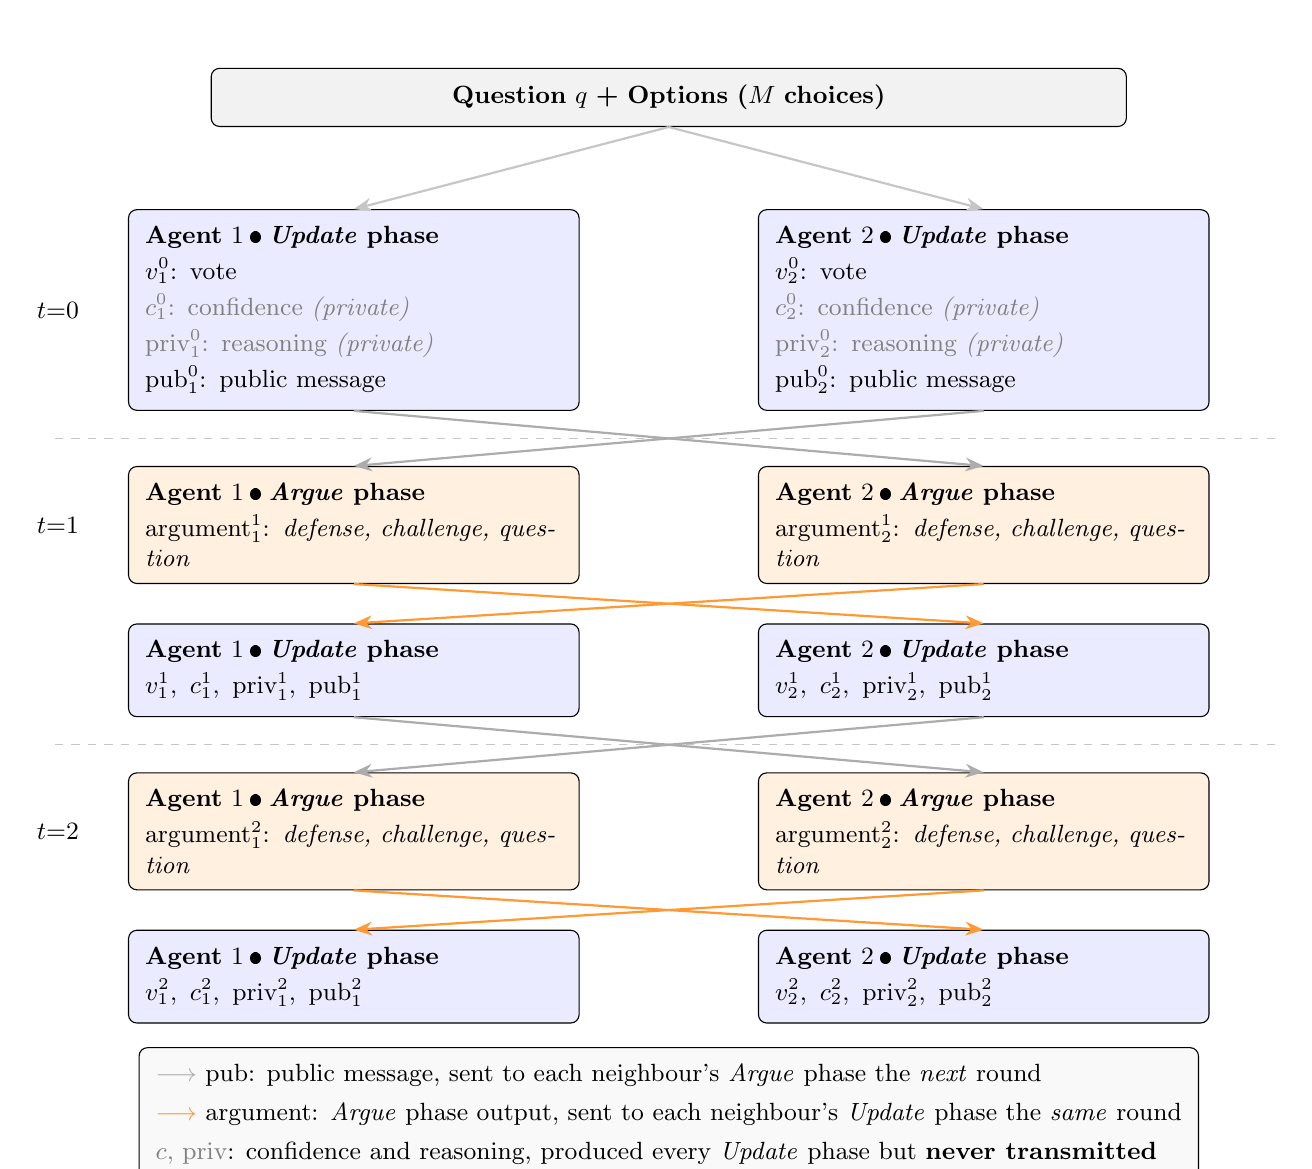
\begin{tikzpicture}[
  font=\small,
  phB/.style={draw, rounded corners=3pt, fill=blue!8, align=left,
              inner sep=6pt, text width=5.3cm},
  phA/.style={draw, rounded corners=3pt, fill=orange!12, align=left,
              inner sep=6pt, text width=5.3cm},
  parr/.style={-Stealth, thick, gray!65},
  darr/.style={-Stealth, thick, orange!80},
  >=Stealth
]

\coordinate (Lsep) at (-3.8, 0);
\coordinate (Rsep) at (11.8, 0);

% Question box
\node[draw, rounded corners=3pt, fill=gray!10, align=center,
      inner sep=6pt, text width=11.2cm] (Q) at (4.0, 2.7) {
  \textbf{Question $q$ + Options ($M$ choices)}
};

% r=0 --- Phase B only
\node[phB] (B0i1) at (0, 0) {
  \textbf{Agent $1$\,\textbullet\,\updatephase{} phase}\\[2pt]
  $v_1^{0}$: vote\\[2pt]
  {\color{gray}$c_1^{0}$: confidence \textit{(private)}}\\[2pt]
  {\color{gray}$\text{priv}_1^{0}$: reasoning \textit{(private)}}\\[2pt]
  $\text{pub}_1^{0}$: public message
};
\node[phB] (B0i2) at (8.0, 0) {
  \textbf{Agent $2$\,\textbullet\,\updatephase{} phase}\\[2pt]
  $v_2^{0}$: vote\\[2pt]
  {\color{gray}$c_2^{0}$: confidence \textit{(private)}}\\[2pt]
  {\color{gray}$\text{priv}_2^{0}$: reasoning \textit{(private)}}\\[2pt]
  $\text{pub}_2^{0}$: public message
};
\node[font=\bfseries\small, left=0.5cm of B0i1] {$t{=}0$};
\draw[-Stealth, thick, gray!45] (Q.south) -- (B0i1.north);
\draw[-Stealth, thick, gray!45] (Q.south) -- (B0i2.north);

\path (B0i1.south) +(0,-0.35) coordinate (sep01);
\draw[dashed, gray!45, thin] (Lsep |- sep01) -- (Rsep |- sep01);

% r=1 --- Phase A
\node[phA, below=0.7cm of B0i1] (Ar1i1) {
  \textbf{Agent $1$\,\textbullet\,\arguephase{} phase}\\[2pt]
  $\text{argument}_1^{1}$: \textit{defense, challenge, question}
};
\node[phA, below=0.7cm of B0i2] (Ar1i2) {
  \textbf{Agent $2$\,\textbullet\,\arguephase{} phase}\\[2pt]
  $\text{argument}_2^{1}$: \textit{defense, challenge, question}
};
\node[font=\bfseries\small, left=0.5cm of Ar1i1] {$t{=}1$};
\draw[parr] (B0i1.south) -- (Ar1i2.north);
\draw[parr] (B0i2.south) -- (Ar1i1.north);

% r=1 --- Phase B
\node[phB, below=0.5cm of Ar1i1] (Br1i1) {
  \textbf{Agent $1$\,\textbullet\,\updatephase{} phase}\\[2pt]
  $v_1^{1},\ c_1^{1},\ \text{priv}_1^{1},\ \text{pub}_1^{1}$
};
\node[phB, below=0.5cm of Ar1i2] (Br1i2) {
  \textbf{Agent $2$\,\textbullet\,\updatephase{} phase}\\[2pt]
  $v_2^{1},\ c_2^{1},\ \text{priv}_2^{1},\ \text{pub}_2^{1}$
};
\draw[darr] (Ar1i1.south) -- (Br1i2.north);
\draw[darr] (Ar1i2.south) -- (Br1i1.north);

\path (Br1i1.south) +(0,-0.35) coordinate (sep12);
\draw[dashed, gray!45, thin] (Lsep |- sep12) -- (Rsep |- sep12);

% r=2 --- Phase A
\node[phA, below=0.7cm of Br1i1] (Ar2i1) {
  \textbf{Agent $1$\,\textbullet\,\arguephase{} phase}\\[2pt]
  $\text{argument}_1^{2}$: \textit{defense, challenge, question}
};
\node[phA, below=0.7cm of Br1i2] (Ar2i2) {
  \textbf{Agent $2$\,\textbullet\,\arguephase{} phase}\\[2pt]
  $\text{argument}_2^{2}$: \textit{defense, challenge, question}
};
\node[font=\bfseries\small, left=0.5cm of Ar2i1] {$t{=}2$};
\draw[parr] (Br1i1.south) -- (Ar2i2.north);
\draw[parr] (Br1i2.south) -- (Ar2i1.north);

% r=2 --- Phase B
\node[phB, below=0.5cm of Ar2i1] (Br2i1) {
  \textbf{Agent $1$\,\textbullet\,\updatephase{} phase}\\[2pt]
  $v_1^{2},\ c_1^{2},\ \text{priv}_1^{2},\ \text{pub}_1^{2}$
};
\node[phB, below=0.5cm of Ar2i2] (Br2i2) {
  \textbf{Agent $2$\,\textbullet\,\updatephase{} phase}\\[2pt]
  $v_2^{2},\ c_2^{2},\ \text{priv}_2^{2},\ \text{pub}_2^{2}$
};
\draw[darr] (Ar2i1.south) -- (Br2i2.north);
\draw[darr] (Ar2i2.south) -- (Br2i1.north);

% Legend
\coordinate (legX) at (4.0, 0);
\path (Br2i1.south) +(0,-1.15) coordinate (legY);
\node[draw, rounded corners=3pt, fill=gray!5, align=left, inner sep=6pt]
  at (legX |- legY) {%
  {\color{gray!65}$\longrightarrow$}~$\text{pub}$: public message, sent to each
    neighbour's \arguephase{} phase the \emph{next} round\\[3pt]
  {\color{orange!80}$\longrightarrow$}~$\text{argument}$: \arguephase{} phase output, sent to
    each neighbour's \updatephase{} phase the \emph{same} round\\[3pt]
  {\color{gray}$c$, $\text{priv}$}: confidence and reasoning, produced every
    \updatephase{} phase but \textbf{never transmitted}%
};

\end{tikzpicture}
\caption[Two-phase synchronous debate protocol]{Two-phase synchronous protocol illustrated for two agents over rounds
$t{=}0,1,2$. As round~$0$ has no \arguephase{} phase, the agents read
the question directly. Each \updatephase{} phase commits the four state fields
$(v,c,\text{priv},\text{pub})$; the confidence $c$ and reasoning $\text{priv}$
stay private (grey). A public message reaches neighbours in the \emph{next}
round's \arguephase{} phase; an \arguephase{} argument reaches neighbours in the \emph{same} round's
\updatephase{} phase, which is what lets one round carry a full question--answer exchange.}
\label{fig:protocol}
\end{figure}

The two-phase structure compresses a question--answer exchange into a single
round as a one-phase synchronous protocol could not achieve this without a
two-round lag. For the dynamical analysis, only the committed \updatephase{} state is
treated as the system state at round $t$; the arguments mainly function as message memory and debate facilitator. All outputs are returned as structured JSON and no problems with malformed responses were observed. The complete prompt templates are shown in \autoref{app:prompts}.

\label{sec:setup:protocol:memory}%
One aspect of the round structure left unspecified so far is how much history each
agent may access. The memory window $W \in \mathbb{Z}_{\geq 1}$ controls how many past rounds each agent sees. At round $t$, agent $i$ has a \emph{self} window of its
own recent states and arguments, and a \emph{peer} window of its neighbours' recent
votes, public messages, and arguments:
\begin{align}
  \mathcal{H}^{\text{self}}_i(t, W)
    &= \big\{\big(v_i^{t-k},\, c_i^{t-k},\, \text{pub}_i^{t-k},\, \text{argument}_i^{t-k}\big)\big\}_{k=1}^{\min(t,\,W)}, \\
  \mathcal{H}^{\text{peer}}_i(t, W)
    &= \big\{\big(v_j^{t-k},\, \text{pub}_j^{t-k},\, \text{argument}_j^{t-k}\big)\big\}_{j \in \mathcal{N}(i),\ k=1..\min(t,\,W)}.
\end{align}
Peer entries are presented in randomised order at each call to mitigate position
bias \citep{zheng2024selectors}, and round-$0$ entries omit the argument field, which does not exist yet. A larger memory window
$W$ exposes more history but also interacts with documented long-context
degradation \citep{liu2024lostmiddle}, which is why we treat $W$ as an explicit
perturbation axis rather than fixing it implicitly. $W = 1$ is the near-Markov
baseline in which each agent sees only the previous round.

Now that the protocol and memory structure are defined, the remaining question is when to stop.
Running every repetition for the full $T$ rounds is wasteful once agents have
converged: pilot transition matrices show a self-loop probability of $0.97$--$1.00$
for the unanimous states, meaning that once consensus is reached, escape is rare.
We therefore stop a repetition as soon as $u$ consecutive rounds are
unanimously agreed. The threshold $u$ trades efficiency against reliability: too
small and a transient consensus may be cut short; too large and the savings
shrink. Analysing pilot repetitions (see \autoref{fig:time_savings} in the appendix), we find that the
harmful case, in which stopping would have prevented a later recovery to the
correct answer, stays negligible while coverage remains high, and we set $u = 3$
with a hard cap of $T = 15$. 
Terminating debate at consensus is standard practice
in the MAD literature \citep{yin2023eot, yang2025revisiting, kaesberg2025voting}.

When a repetition ends, the system's answer is the \emph{plurality} of the agents' votes
at the final round, the option held by the most agents. Because a repetition stops
only after $u = 3$ consecutive unanimous rounds, every converged repetition ends
with all $N$ agents on one option, so the plurality is unambiguous and equals that
option. A tie can therefore arise only in the rare repetitions that reach the hard
cap $T = 15$ without converging, which occurs in approximately $2\,\%$ of repetitions. Such ties are broken deterministically towards the first option in
canonical order. The resulting label is a low-confidence artefact of wherever the
unresolved run happened to land rather than a genuine group decision, and
\autoref{sec:results:lc} recommends flagging these repetitions as unresolved
instead of trusting the reported majority.

% ------------------------------------------------------------
% Commented out but retained in case it is needed later.
% ------------------------------------------------------------
% \paragraph{Early task stopping.}
% Not every question is worth its full repetition budget. For some, all agents are
% already unanimous at $t = 0$, so the outcome is fixed by the model's prior rather
% than by deliberation. Using a small pilot batch of $R_{\text{pilot}} = 5$
% repetitions, we skip the remainder of a task if the mean per-agent accuracy at
% $t = 0$ and the mean system accuracy at the final round agree at an extreme:
% \begin{equation}
%   \big(\bar{a}_0 \geq \theta_{\text{high}} \ \text{and}\ \bar{a}_T \geq \theta_{\text{high}}\big)
%   \quad\text{or}\quad
%   \big(\bar{a}_0 \leq \theta_{\text{low}} \ \text{and}\ \bar{a}_T \leq \theta_{\text{low}}\big),
% \end{equation}
% with $\theta_{\text{high}} = 0.95$ (trivially easy) and $\theta_{\text{low}} = 0.05$
% (effectively unsolvable). Requiring agreement between $t = 0$ and the final round
% prevents false positives, since a question whose accuracy moves between the two
% cannot satisfy either condition. The unanimously-correct case is safe to filter
% unconditionally (a correct consensus at $t = 0$ is stable under the dynamics);
% the unanimously-wrong case is in principle riskier, but recovery from it was
% observed in only one of twenty pilot questions.


% ------------------------------------------------------------
% 4.3 DATASETS
% ------------------------------------------------------------
\subsection{Datasets}
\label{sec:setup:datasets}

Because this work studies motif emergence rather than task-completion
performance, our benchmark selection criteria differ from those usual in the MAD
literature. A benchmark suitable for motif detection must provide (i) a
\textbf{discrete shared decision variable}, so that all agents commit to a
position in the same finite set each round; (ii) \textbf{verifiable ground truth},
so dynamics can be related to correctness; (iii) \textbf{calibrated difficulty},
since saturated tasks remove the disagreement that drives deliberation; and (iv)
\textbf{sufficient initial disagreement}, without which no motif can be
distinguished from trivial consensus.

Applying these criteria rules out most existing benchmarks. Saturated reasoning
sets such as GSM8K and MMLU leave no headroom for deliberation dynamics; native
multi-agent benchmarks are largely incompatible, being either role-specialised
or defined over spatial rather than categorical positions. A full survey of the candidates we considered and the reason each was
rejected is given in \autoref{app:benchmarks}. Two bench satisfy all four
criteria and are complementary, so we use them throughout this study.

\paragraph{GPQA-Diamond.}
\label{sec:setup:datasets:gpqa}
GPQA-Diamond \citep{rein2024gpqa} is a graduate-level science
question-answering benchmark of 198 questions in biology, physics, and
chemistry, written by domain experts and validated through a ``Google-proof''
protocol that resists retrieval-based shortcuts. It satisfies all four criteria
directly: four-option multiple choice ($M = 4$) provides the discrete decision
variable; expert validation gives unambiguous ground truth; frontier models fall
well below ceiling \citep{rein2024gpqa, becker2025orchestration}, leaving genuine
headroom for debate; and agents genuinely disagree at round one
\citep{becker2025orchestration}.
GPQA-Diamond also has direct multi-agent precedent
\citep{becker2025orchestration, kenton2024debate, he2025dimo, wang2025mars}. We
adopt it as the \textbf{primary} dataset. 
The main cavueat is that this benchmark has less cumulative MAD literature compared to MMLU or GSM8K, which is however mostly the case as its a moer recent benchmark and not because of a methodological pivot. 
A second caveat concerns comparability of the accuracy numbers: published figures
refer to strong models on the full benchmark, whereas we use
a mid-tier model on a screened task subset only.
Our results are therefore not comparable to published frontier GPQA-Diamond
numbers, and are not intended to be; the screening pass deliberately selects the
most dynamically contested tasks, where accuracy is low by design.

\paragraph{HiddenBench.}
\label{sec:setup:datasets:hiddenbench}
Moreover, we use HiddenBench \citep{li2026hiddenbench} as a structurally complementary
\textbf{secondary} dataset. It formalises the
hidden-profile paradigm from social psychology
\citep{stasser1985pooling, schulzhardt2012synergy}, in which the evidence needed for the
correct answer is split across agents, so that no single agent can solve the task
alone and success requires information pooling. Its value here is as a
control for a specific confound. Motifs seen only on GPQA-Diamond might be
artefacts of cooperative reasoning over a reliable individual signal, in which
RLHF-induced truth-seeking \citep{ouyang2022instructgpt} amplifies convergence.
Under the hidden-profile condition, by contrast, pre-discussion accuracy is very
low by construction \citep{li2026hiddenbench}, so any post-discussion improvement
must come from social information transfer rather than from individual competence.
Motifs that appear on both datasets are therefore robust to this confound,
while motifs that appear on only one are themselves informative on a dataset-level.

One structural detail of HiddenBench matters for the analysis. While we use
$N = 4$ agents throughout, the number of answer options is task-dependent,
$M \in \{3, 4\}$. The agent count $N$ and the option count $M$ are therefore
independent quantities and should not be conflated. This is why every
option-indexed quantity in \autoref{sec:method} is defined over the task's actual
$M$ options.
Extension to mixed-motive negotiation datasetes is left to future work.


% ------------------------------------------------------------
% 4.4 EXPERIMENTAL DESIGN
% ------------------------------------------------------------
\subsection{Experimental Design}
\label{sec:setup:design}

The system exposes many tunable components. We classify each as \textbf{scan} (a
primary perturbation axis), \textbf{fix} (held constant), or \textbf{defer} (out
of scope). \autoref{tab:knob-summary} summarises the classification and the
literature supporting it; the detailed per-knob justification is deferred to
\autoref{app:knobs}.

Of these components, two are varied as primary perturbation axes, chosen because they
are the canonical levers for network-motif analysis:
\begin{itemize}
  \item \textbf{Memory window} $W \in \{1, 2, 5\}$, with $W = 1$ the near-Markov
        baseline. Memory content is an established driver of debate behaviour
        \citep{du2024improving, li2024sparsetopology}.
  \item \textbf{Topology} $\in \{\textsc{fc}, \textsc{star}\}$. Fully-connected
        probes the symmetric baseline; the star probes hub-induced dominance,
        following evidence that centralised structures concentrate influence
        \citep{li2024sparsetopology, chen2023consensus, liu2025problemsolving}.
\end{itemize}
Their product gives $3 \times 2 = 6$ configurations per task. The dataset (GPQA
or HiddenBench) is classified as a scanned condition in \autoref{tab:knob-summary}
because the information condition varies between benchmarks, but it is not a
structural axis in the sense of a manipulation applied within a fixed task; the
two benchmarks are instead analysed separately. The full design
therefore spans $6 \times 2 = 12$ configuration--dataset cells.
All remaining components are held constant to isolate the effect of the two scan
axes:
\begin{itemize}
  \item \textbf{Agents} $N = 4$: the smallest value at which the two
        topologies are structurally distinct and multi-way splits can occur.
  \item \textbf{Rounds} $T = 15$ (hard cap) with early stopping $u = 3$: $T$ is
        an observation budget rather than a structural knob, since trajectories
        can be cropped post hoc but not extended.
  \item \textbf{Model} \texttt{mistral-medium-instruct}: a single mid-tier
        model to isolate topology and memory effects from capability-asymmetry
        effects of heterogeneous models \citep{wynn2025talk}.
  \item \textbf{Sampling} temperature $0.7$, reasoning disabled: diverse yet
        focused outputs, avoiding the degenerate identical-sample case
        \citep{zhu2026demystifying}.
  \item \textbf{Framing} cooperative, with the full \arguephase{}/\updatephase{} structured
        output as the measurement instrument, and synchronous execution to
        remove agent-order confounds.
\end{itemize}

Finally, selecting which tasks to run completes the design. Motifs are per-task properties, and running the full grid at high $R$ on every
question is infeasible: at roughly $25$\,s per repetition, the full GPQA-Diamond
set across six configurations would take approximately $10.3$ days ($248$\,h) at
$R = 30$ or $17.2$ days ($413$\,h) at the final $R = 50$; a two-phase design that 
employs an initial screening process reduces this to approximately $29$\,h. 
It begins with a shallow \emph{screening} pass which runs every task once at a
single baseline configuration (\textsc{fc}, $W = 1$, $R = 3$) and retains only
those tasks where debate actually occurs \emph{and} the final answer varies
across repetitions, since only those tasks have dynamics, rather than the model
prior, deciding the outcome. Tasks that are unanimous at $t = 0$, that always
converge to the same answer, or where no genuine disagreement arises, are
excluded.

\begin{table}[H]
\centering
\small
\begin{tabular}{p{3.0cm}lp{4.4cm}p{4.8cm}}
\toprule
\textbf{Knob} & \textbf{Verdict} & \textbf{Value} & \textbf{Key references} \\
\midrule
Memory $W$ & scan & $\{1, 2, 5\}$ & \citep{du2024improving, li2024sparsetopology} \\
Topology & scan & fc, star & \citep{li2024sparsetopology, chen2023consensus, liu2025problemsolving} \\
Agents $N$ & fix & $4$ & \citep{du2024improving, li2026hiddenbench} \\
Rounds $T$ & fix & $15$ (cap), $u=3$ & \citep{kaesberg2025voting, yang2025revisiting} \\
Output structure & fix & full \arguephase{}/\updatephase{} & \citep{liang2024encouraging, he2025dimo} \\
Framing & fix & cooperative & \citep{liang2024encouraging, du2024improving} \\
Synchrony & fix & parallel-synchronous & \citep{du2024improving, liu2024groupdebate} \\
Model & fix & \texttt{mistral-medium-instruct} & \citep{liu2025stopovervaluing, wynn2025talk} \\
Temperature & fix & $0.7$, no reasoning & \citep{zhu2026demystifying} \\
Information cond. & scan (dataset) & GPQA ($M{=}4$), HiddenBench ($M{\in}\{3,4\}$) & \citep{li2026hiddenbench, stasser1985pooling} \\
Tool access & defer & none & \citep{rein2024gpqa} \\
\bottomrule
\end{tabular}
\caption[Classification of tunable components]{Classification of tunable components. Full justification per knob is
given in \autoref{app:knobs}.}
\label{tab:knob-summary}
\end{table}

Retained tasks are promoted to a deep \emph{characterisation} pass on the full
six-configuration grid. This yields the final dataset used throughout
\autoref{sec:results}: \textbf{50 tasks for each of the two benchmarks, six
configurations each, $R = 50$ repetitions}, for a total of
$50 \times 2 \times 6 \times 50 = 30{,}000$ repetitions.
GPQA-Diamond yields more eligible tasks than needed in the screening pass, so we
retain $50$ to match the number of eligible HiddenBench tasks, giving a balanced
design with equal task counts per benchmark; the $50$ are drawn uniformly at
random from the eligible GPQA tasks, so that no further selection is made on any
outcome-derived quantity. Because $R = 3$ in the screening pass introduces some
noise, assignments near the inclusion boundary are mildly unstable, which we
accept as a screening cost rather than a final claim.

One consequence of this design should be made explicit for the interpretation of
RQ2. Because the characterisation pass runs only tasks selected by the screening
procedure, raw task difficulty is held roughly constant by construction: it is a
\emph{selection criterion} for the study rather than a factor we vary within it.
The ``difficulty regime'' contrast that RQ2 refers to is therefore operationalised
at the benchmark level, GPQA (a refinement regime, agents mostly start correct)
versus HiddenBench (a correction regime, agents start systematically wrong).
A further interpretive consequence concerns bistability. Because tasks are
retained precisely because their final answer varies across repetitions under the
screening configuration, the prevalence of coexisting attractors reported in
\autoref{sec:results:bistability} is conditioned on this selection and should not
be read as an estimate of motif frequency in an unselected task population; see
\autoref{sec:discussion:limitations} for discussion.

Code, prompts, and run scripts are
available at \url{https://github.com/echtermeyer/LLM-Based-MAS}.

\newpage

\section{Detection Methodology}
\label{sec:method}
% ============================================================
% CHAPTER 5: DETECTION METHODOLOGY
%
% Structure (matches ToC):
%   5.1  Shared Measurement Conventions
%   5.2  Self-Reinforcement
%   5.3  Multistability
%   5.4  Dominance
%   5.5  Limit Cycles          (subsubsections collapsed)
%
% Every detector subsection follows the same five moves:
%   Concept -> Measurement -> Detection -> Worked example -> Limitations
% Split rule: Measurement is what we compute from the log; Detection is
% the null it is tested against and the rule that flags the motif.
%
% Notation is unified with Chapter 4:
%   t = round index, r = repetition, N = agents (=4), M = options
%   v_i^t = vote, c_i^t = confidence, s_t = macrostate.
% Recurrence-matrix positions are indexed by (a,b) to avoid clashing
% with the agent index i.
%
% REMOVED LABELS (redirect any \autoref pointing at them to
% \autoref{sec:method:lc}):
%   sec:method:lc:agent
%   sec:method:lc:system
%
% Persuasiveness and message alignment are retained (commented out at
% the end of this file) for later reference but are no longer part of
% the methodology. Per-detector implementation notes and the list of
% future motifs are moved to the appendix.
% ============================================================


Each of the four motifs defined in this section is a hypothesis about the
underlying debate dynamics. If the system self-organizes in the way a
complex-systems reading predicts, then confidence should reinforce within a held
position, repeated repetitions should settle into a small number of
initial-condition-selected attractors, influence should concentrate on particular
agents, and in some configurations vote sequences may oscillate persistently
without converging. This section turns each hypothesis into a \emph{detector}: a
statistic computed from the interaction log together with a principled null model
against which it is tested, so that a positive result reflects genuine structure
rather than the chance regularities of a small, discrete state space. Together the
four detectors form \suitename{}, the detector suite this thesis contributes.

Two properties are shared by all four detectors and therefore are worth stating up
front. Firstly, each detector reads only from ordinary interaction logs, the vote
and confidence channels defined in \autoref{sec:exp}, which is what later lets us
propose the same detectors as diagnostic instruments. And secondly, each detects a
\emph{signature}, not a certified dynamical object. Thus, we add a
``Limitations'' paragraph to each detector which makes explicit what the
corresponding statistic can and cannot claim.


% ------------------------------------------------------------
% 5.1 SHARED MEASUREMENT CONVENTIONS
% ------------------------------------------------------------
\subsection{Shared Measurement Conventions}
\label{sec:method:vocab}

Before defining each detector individually, it is worth fixing what they share.
Four things recur across every subsection below: the shape those subsections take,
the classification of the motifs themselves, the macrostate the system-level
detectors read from, and the nesting of the data that constrains every comparison.

The four subsections each make the same five moves, in the same order.
\emph{Concept} states the motif in dynamical-systems terms and names the quantity
in a debate that plays the role of the state variable. \emph{Measurement} defines
the \emph{measurement primitive}, the lowest-level object the detector scores, and
the statistic computed from it. \emph{Detection} gives the null model that
statistic is tested against and the rule that flags the motif. \emph{Worked
example} runs the detector by hand on a small case, and \emph{Limitations} states
what the resulting statistic cannot claim. The division between the second and
third move is the one worth holding on to, since it recurs throughout: measurement
is what we compute from the log, detection is what we compare it against. So that
the four worked examples can be read against one another, they share a single
running scenario, one task with $N = 4$ agents and $M = 4$ options labelled $A$ to
$D$ of which $A$ is correct, and they write an agent's state as its option with its
confidence as a subscript, so that $D_8$ is a vote for $D$ held at confidence $8$.

The motifs those subsections detect are preselected rather than exhaustively
enumerated, each motivated by a documented failure mode of LLM-based debate.
\autoref{tab:method:motifs} lists them together with their classification and the
section in which each detector is defined. Further motifs that fall within the same
structural-dynamical framework but lie outside the scope of this study are catalogued
in Appendix~\ref{app:future_motifs}.

\begin{table}[H]
\centering
\small
\begin{tabular}{llll}
\toprule
Motif & Classification & Level & Section \\
\midrule
Self-reinforcement & Structural (positive autoregulation) & Agent & \autoref{sec:method:sr} \\
Multistability        & Dynamical (coexisting attractors)    & System & \autoref{sec:method:multistability} \\
Dominance          & Structural (emergent hub)            & System & \autoref{sec:method:dominance} \\
Limit cycle        & Dynamical (periodic orbit)           & Agent \& System & \autoref{sec:method:lc} \\
\bottomrule
\end{tabular}
\caption[Motif classification]{The four motifs classified by type (structural or dynamical, following
\autoref{sec:bg:motifs}) and level (whether the detector reads from individual
agent trajectories, the collective macrostate, or both).}
\label{tab:method:motifs}
\end{table}

What the table calls the \emph{level} of a motif decides where its detector reads
from. Self-reinforcement, the only agent-level motif, reads directly from
per-agent vote and confidence trajectories. The three system-level readings
instead operate on the agent-anonymised macrostate $s_t$ defined in
\autoref{sec:setup:notation}, whose key property is that composition retains more
information than a plain vote count: a $3$--$1$ split and a $2$--$2$ split are
distinct macrostates, and options remain labelled because one is correct and they
are not interchangeable. Each of the three takes a different slice of that record,
however. Multistability reads only the locked-in endpoint, dominance reads the
emergent influence graph, which is built relationally and therefore needs
within-repetition agent identity, and the system-level limit-cycle test reads the
full sequence $s_0, \ldots, s_T$.

Whichever slice a detector takes, it inherits the same nesting of the data,
\begin{equation}
  \text{agent} \subset \text{repetition} \subset \text{task} \subset
  \text{config } (W \times \text{topology}) \subset \text{dataset},
\end{equation}
with $W \in \{1,2,5\}$, $\text{topology} \in \{\text{fc}, \text{star}\}$, $N = 4$,
and $\text{dataset} \in \{\text{GPQA}, \text{HiddenBench}\}$, and that nesting
constrains what may be compared with what. Because agents interact within a
repetition, their trajectories are not independent, so the repetition is the
independent unit of replication and agent-level trajectories are never pooled as
if they were separate observations (pseudoreplication). For the same reason GPQA
and HiddenBench are always analysed separately and never pooled, and memory-window
comparisons are made within a fixed topology and dataset, since cells from
different configs are not exchangeable.

A last property is shared by all four detectors, and it bounds every claim they
make: each is phenomenological rather than causal. We detect a trajectory or
influence \emph{signature}, not a certified attractor, cycle, or causal hub, and
separating the signature from its underlying cause requires dedicated perturbation
experiments, which we leave to future work. Under the cooperative,
convergence-forced design we also expect several detectors to return sparse or
near-null results, which is why each detection paragraph below names the baseline
its statistic is compared against rather than testing it against zero.


% ------------------------------------------------------------
% 5.2 SELF-REINFORCEMENT
% ------------------------------------------------------------
\subsection{Self-Reinforcement}
\label{sec:method:sr}

\paragraph{Concept.}
In complex systems, self-reinforcement is \emph{positive feedback}: the current
level of a state variable raises the drive toward more of the same, so deviations
are amplified rather than damped \citep{arthur1989competing}. At the motif level
this is positive autoregulation, a node that augments its own production
\citep{milo2002network, alon2007network}. For us the state variable is an agent's
expressed \emph{confidence}. Self-reinforcement is then the tendency of an agent
to push its own confidence upward while it holds a position, driven by
accumulating commitment rather than by what the incoming information warrants. The
pattern is already documented: in multi-turn LLM debate, confidence tends to rise
across rounds in an anti-Bayesian fashion, even where no new information justifies
the rise \citep{prasad2025certain}.

For the detection of self-reinforcement a rising confidence trajectory is on its
own necessary but not sufficient, since rational updating and peer conformity also
push confidence up. We therefore measure two signatures that go beyond it.
\emph{Directional drift} is the tendency of confidence to increase rather than
decrease while a position is held. \emph{Strength scaling} is the prediction that
this drift grows with how strongly an agent is re-exposed to its own prior
commitments, which the memory window $W$ controls directly. A third signature,
\emph{endogeneity}, would establish that the rise comes from the agent's own
commitment rather than from new information, but it cannot be separated from peer
effects using trajectory data alone.

\paragraph{Measurement.}
The primitive is the \emph{vote-stable segment}: a maximal block of consecutive
rounds over which agent $i$'s vote does not change, running from its start $t_s$
to its end $t_e$, so that $v_i^t = v_i^{t_s}$ for all $t \in \{t_s, \ldots, t_e\}$.
Writing $L = t_e - t_s + 1$ for its length in rounds, a segment is retained only if
$L \geq 3$. Two rounds would already define a slope, but that slope would be a
single confidence difference with no residual degrees of freedom, so its sign would
turn on one integer step; three rounds give two steps for the least-squares fit to
average over. An agent might contribute several segments if it flips and one long
segment if it locks in early. Agents are exchangeable, so segments are pooled
within a config and never matched across repetitions.
Within a retained segment we regress confidence on the round index by ordinary
least squares,
\begin{equation}
  c_i^t = \beta_0 + \beta_{\mathrm{seg}}\, t + \varepsilon_t,
  \qquad t \in \{t_s, \ldots, t_e\},
\end{equation}
and keep the slope $\beta_{\mathrm{seg}}$, in confidence points per round. Its sign
feeds the prevalence test below, and its signed value feeds the mean slope
$\bar{\beta}$ used in the $W$ comparison.

\paragraph{Detection.}
With the segments in hand, the question is whether their slopes lean upward more
often than chance allows. We read them in two ways, both conditioned on the
config.
The first is a presence test for directional drift. Writing $n_{\mathrm{seg}}$ for
the number of retained segments in a config-task pair, the prevalence of upward
segments is
\begin{equation}
  \hat{p}_{\mathrm{SR}}
  = \frac{\bigl|\{\text{seg}: \beta_{\mathrm{seg}} > 0\}\bigr|}{n_{\mathrm{seg}}},
\end{equation}
so flat segments ($\beta_{\mathrm{seg}} = 0$) sit in the denominator but never in
the numerator. Under a no-feedback ``wobble'' null an upward and a downward
segment are equally likely, so with a fraction $f$ of flat segments
$P(\beta_{\mathrm{seg}} > 0) = \tfrac{1}{2}(1-f) \leq 0.5$. Thus, self-reinforcement is
indicated when $\hat{p}_{\mathrm{SR}} > 0.5$. Both the flat segments and the
confidence ceiling, since a segment already at the top of the scale cannot drift
further up, make a positive result conservative.
The second reading uses the memory window to discriminate between mechanisms.
Letting $\bar{\beta}$ be the mean segment slope in a config, an \emph{endogenous}
reading predicts that re-reading one's own prior commitments across a longer
window amplifies the internal drive,
\begin{equation}
  \bar{\beta}(W{=}5) > \bar{\beta}(W{=}2) > \bar{\beta}(W{=}1),
\end{equation}
whereas under a \emph{peer-conformity} reading a longer window mainly adds peer
content, and the ordering may be absent or reversed. 

Both readings are reported per config-task and then summarised across tasks,
for example ``above $0.5$ in $k$ of $50$ tasks'', so that an effect is shown to be
broad rather than driven by one task.

\paragraph{Worked example.}
In the running scenario, suppose agent~$0$ holds option~$A$ for five rounds with
confidences $c = (5, 6, 6, 8, 9)$. This is one vote-stable segment of length
$L = 5$, and regressing confidence on the round index gives
$\beta_{\mathrm{seg}} = +1.0$ confidence points per round: an upward segment,
counting toward $\hat{p}_{\mathrm{SR}}$. Had the agent instead drifted
$c = (7, 7, 6, 6, 5)$, the slope would be $-0.5$ and the segment would count
against it. A segment that never moved, $c = (6,6,6,6,6)$, has
$\beta_{\mathrm{seg}} = 0$: retained in the denominator but not counted as upward,
which is what makes the $0.5$ reference conservative. Under the strength-scaling
reading, the average of such slopes should grow as the window widens from
$W{=}1$ to $W{=}5$.

\paragraph{Limitations.}
Beyond the shared phenomenological caveat, two points bound the claim.
\emph{Endogeneity is not isolated}: an upward segment is equally consistent with
peer copying and with a peer surfacing genuinely new information in a later round,
and rising confidence alone cannot tell these apart. The $W$ ordering narrows the
ambiguity but does not settle it, since a longer window also re-exposes more peer
content. \emph{Convergence is a confound}: on easier tasks fast agreement can
itself raise confidence, which is why prevalence is reported per task and never as
a single pooled figure.


% ------------------------------------------------------------
% 5.3 MULTISTABILITY
% ------------------------------------------------------------
\subsection{Multistability}
\label{sec:method:multistability}

\paragraph{Concept.}
In dynamical systems, \emph{multistability} is the coexistence of two or more
stable attractors for one fixed parameter set. Into which attractor the system settles
into is decided by the basin of attraction containing the initial condition
\citep{feudel2008complex, pisarchik2014control}. At the motif level this is the dynamical signature of positive
feedback with a symmetry: the same interaction rules admit several self-consistent
outcomes \citep{milo2002network, alon2007network}. For us the state variable is
the macrostate $s_t$, and multistability is read off the \emph{locked-in endpoint}:
for a fixed task, the debate converges to different consensus answers on different
repetitions, and which one is reached is selected by the initial vote
configuration rather than by the task's correct option. This is the structural
reading of unreliable correction: on a task where the model carries a systematic
bias, a wrong-consensus and a right-consensus attractor can coexist, and the
group's fate is basin competition decided at round $0$, which self-reinforcement
then amplifies and locks in. For the motif detection, seeing more than one final answer is necessary but
not sufficient, as a task may simply be noisy. Thus, genuine multistability
additionally requires that the initial condition \emph{predicts} the endpoint
\citep{pisarchik2014control}.

\paragraph{Measurement.}
The primitive and independent unit is the repetition, characterised by its initial
vote composition $s_0 = (n_1^0,\ldots,n_M^0)$ and its final macrostate. A
repetition is converged if its final macrostate is unanimous, regardless
of whether that unanimity was reached via early stopping or at the round cap $T$.
We restrict the multistability analysis to converged repetitions because a stable
non-unanimous endpoint reflects a failure to reach collective agreement rather than
a genuine attractor. The endpoint attractor $A^{(r)}$ of a converged repetition is
the winning option, so there are at most $M$ distinct attractors per task.
Repetitions that end in a non-unanimous state are excluded.
Scoring is per task-config cell with $n_c$ denoting the number of converged
repetitions in that cell. The cell's \emph{dominant attractor} is the most
frequent endpoint option, and each repetition's start is summarised by
\begin{equation}
  g(s_0) \in \{0, 1, \ldots, N\},
\end{equation}
the number of agents whose round-$0$ vote is on the dominant option.
From these we compute the empirical basin distribution over endpoint attractors,
$\hat{P}(A = k) = \tfrac{1}{n_c}\sum_r \mathbf{1}[A^{(r)} = k]$, a basin-stability
estimate of relative basin volumes under the model's own initial distribution
\citep{menck2013basin}. The effective number of coexisting attractors is the
inverse Simpson (Hill) index \citep{hill1973diversity},
\begin{equation}
  N_{\mathrm{eff}} = \frac{1}{\sum_k \hat{P}(A = k)^2} \in [1, M].
\end{equation}
$N_{\mathrm{eff}} \approx 1$ is a single attractor, $\approx 2$ two coexisting
attractors, and so on, so $N_{\mathrm{eff}}$ reports \emph{how many} attractors
coexist. Because attractors are unanimous options, it is bounded by $M$. Since $M$
varies across tasks, we report $N_{\mathrm{eff}}$ raw and compare it only within a
fixed $M$. In practice GPQA is entirely $M = 4$; only HiddenBench
mixes $M = 3$ and $M = 4$, so its $N_{\mathrm{eff}}$ summaries are reported
separately by option count.

\paragraph{Detection.}
Coexistence alone does not establish multistability; the initial condition must
also \emph{select} the attractor \citep{feudel2008complex, pisarchik2014control},
and it is that association which carries the inferential claim. We measure it
between $g(s_0)$ and the endpoint $A$ with Cram\'er's $V$
\citep{cramer1946mathematical} on their contingency table,
\begin{equation}
  V = \sqrt{\frac{\chi^2 / n_c}{\min(R_{\mathrm{tab}} - 1,\, C_{\mathrm{tab}} - 1)}} \in [0, 1],
\end{equation}
where $\chi^2$ is the Pearson statistic and $R_{\mathrm{tab}}, C_{\mathrm{tab}}$
are the table's numbers of rows (distinct $g(s_0)$, at most $N+1$) and columns
(distinct endpoints, at most $M$). $V \approx 0$ means the start is irrelevant;
$V$ near $1$ means the start deterministically selects the endpoint. The null
shuffles the pairing of $g(s_0)$ and $A$ across the $n_c$ repetitions, preserving
both marginals while destroying the start-to-endpoint link
\citep{theiler1992surrogate}; for $B = 1000$ surrogates the add-one one-sided
$p$-value flags basin selection when $p < 0.05$.

The two readings combine into a single cell label,
\begin{equation}
  \text{label}(c) =
  \begin{cases}
    \text{monostable} & N_{\mathrm{eff}} < 1.5,\\[2pt]
    \text{multistable} & N_{\mathrm{eff}} \geq 1.5 \ \wedge\ p < 0.05,\\[2pt]
    \text{stochastic (not multistable)} & N_{\mathrm{eff}} \geq 1.5 \ \wedge\ p \geq 0.05,
  \end{cases}
\end{equation}
with the degree of multistability read from $N_{\mathrm{eff}}$ and capped at $M$.
The cutoff $1.5$ is a reporting threshold, not a test; the inferential claim rests
on $p$. The third case is the essential guard: coexistence without basin selection
is scatter, not multistability. Because per-cell power is limited, results lean on
the across-task distribution of $N_{\mathrm{eff}}$ and $V$ rather than any single
cell.

\paragraph{Worked example.}
In the running scenario, take a cell with $n_c = 30$ converged repetitions whose
dominant attractor is option~$A$. The coexistence reading depends only on the
endpoint distribution, and the label depends on whether the start predicts it.
\begin{itemize}
  \item \textbf{Monostable.} Endpoints $28 \times A$, $2 \times B$ give
        $\hat{P} = (0.933, 0.067)$ and
        $N_{\mathrm{eff}} = 1/(0.933^2 + 0.067^2) \approx 1.14 < 1.5$: one valley.
  \item \textbf{Multistable.} Endpoints $15 \times A$, $15 \times B$ give
        $N_{\mathrm{eff}} = 2.0$. If repetitions starting with more agents on $A$
        (high $g(s_0)$) end on $A$ and those starting with few end on $B$, then
        $V \approx 1$, $p < 0.05$: two basins selected by the start.
  \item \textbf{Tristable.} Endpoints $10 \times A$, $10 \times B$, $10 \times C$
        with the start predicting each give $N_{\mathrm{eff}} \approx 3.0$,
        $p < 0.05$ (the maximal degree for $M = 3$).
  \item \textbf{Stochastic.} Endpoints $15 \times A$, $15 \times B$ again give
        $N_{\mathrm{eff}} = 2.0$, but if $g(s_0)$ is unrelated to the endpoint then
        $V \approx 0$, $p \gg 0.05$: coexistence without basin selection, correctly
        \emph{not} labelled multistable.
\end{itemize}

\paragraph{Limitations.}
First,
classical basin stability draws initial conditions uniformly
\citep{menck2013basin}, whereas our starts come from the model's own round-$0$
distribution, so $\hat{P}(A)$ estimates \emph{effective} basin volume under that
distribution, not geometric volume. Second, because $g(s_0)$ counts agents already
on the eventual dominant option, a high $V$ is consistent both with genuine basin
selection and with ordinary majority-vote persistence; the test detects
start-to-endpoint dependence but does not by itself separate these two mechanisms,
so we read the association as necessary but not mechanistically decisive.


% ------------------------------------------------------------
% 5.4 DOMINANCE
% ------------------------------------------------------------
\subsection{Dominance}
\label{sec:method:dominance}

\paragraph{Concept.}
Dominance is the concentration of directed influence onto a single node, an
\emph{emergent hub} which is a structural motif \citep{milo2002network, alon2007network}
read at the system level, since it is a property of the whole influence
distribution. Its formal home is opinion dynamics. In the DeGroot model
\citep{degroot1974consensus} and its social-power extension, an agent's influence
equals its network centrality, and the group is \emph{autocratic} when these are
maximally nonuniform and \emph{democratic} when uniform \citep{jia2015opinion}.
Dominance is the autocratic side. For us the state variable is the distribution of
influence across the four agents, and dominance is the tendency of that
distribution to concentrate on one of them rather than to spread evenly. When it
does, a single overconfident agent can pull the rest of the group toward its answer
\citep{chen2023consensus, cho2025herd}, degrading collective accuracy even when
the majority would otherwise be correct \citep{wynn2025talk}. To avoid attributing concentration that is simply an artefact of the wiring, we
measure influence for each topology separately. The result is a
concentration signature rather than proof of causation, since an adoption edge
cannot distinguish genuine influence from coincidental agreement.

\paragraph{Measurement.}
The primitive and independent unit is the per-repetition influence graph, which
requires within-repetition agent identity.
Dominance is defined over agents and their conversions, so it is independent of
the option count $M$. A \emph{conversion} occurs when agent $j$ adopts, at
round $t{+}1$, a vote that a disagreeing neighbour $i$ held at round $t$. The
directed edge $i \to j$ accumulates the confidence-weighted conversions of $j$ onto
$i$'s vote, with credit split among the neighbours already holding the target vote,
\begin{equation}
  w_{ij} = \sum_{t} \frac{1}{m_j^t}\,
           \mathbf{1}\!\left[v_j^{t+1} = v_i^{t} \neq v_j^{t}\right] c_j^{t},
  \qquad
  m_j^t = \bigl|\{k \in \mathcal{N}(j) : v_k^{t} = v_j^{t+1}\}\bigr|,
\end{equation}
where $c_j^t$ is the converting agent's confidence, $\mathcal{N}(j)$ its
topological neighbourhood, and the factor $1/m_j^t$ shares credit equally among
all eligible sources. Per-agent influence is the weighted out-strength
$\sigma_i = \sum_j w_{ij}$. We use out-strength rather than eigenvector centrality
\citep{bonacich1972factoring}, which is undefined or degenerate on
non-strongly-connected and acyclic graphs \citep{newman2010networks} and
hub-localises \citep{martin2014localization}. Our graphs are tiny and sparse, 
making out-strength the only always-defined node score.

The statistic is the concentration of the resulting influence-share vector
$p_i = \sigma_i / \sum_k \sigma_k$, measured by the normalised Herfindahl index
\citep{hirschman1964paternity},
\begin{equation}
  D = \frac{\sum_i p_i^2 - \tfrac{1}{N}}{1 - \tfrac{1}{N}} \in [0, 1].
\end{equation}
$D = 0$ is democratic as the agents have equal influence, and $D = 1$ is a single pure hub. $D$ is
undefined when $\sum_k \sigma_k = 0$, that is when no conversion occurs at all,
and such repetitions are excluded.

\paragraph{Detection.}
A high $D$ in the star is uninformative on its own, since the centre is the only
agent a leaf can be converted by and the wiring alone forces concentration. The
null is therefore keyed to topology: it asks how concentrated $D$ would be if, on
this same wiring and these same conversion events, influence were assigned at
random. We use a constrained shuffle in the spirit of Theiler's ``Algorithm~0''
\citep{theiler1992surrogate} that keeps the converting agent, the round, the
weight, and the number of eligible sources fixed, and redraws only the source
\emph{identity}, uniformly among $\mathcal{N}(j)$.
In the fully-connected topology every agent has three neighbours, so the shuffle can reassign any
conversion to any of them and the resulting null is symmetric; concentration above
it is emergent. However, for the star topology a leaf has exactly one neighbour, so a leaf
conversion has only one possible source and the shuffle leaves it unchanged. Where
a repetition is made up of such conversions, every surrogate reproduces the
observed graph and the test can never flag. This makes the star null degenerate, so emergent concentration is identified only in
the fully-connected topology. Raw $D$ is still reported for both, but in the star
it describes the wiring rather than the behaviour.

A repetition is concentrated when its observed $D$ falls in the upper tail of its
own surrogate distribution. With $B = 1000$ surrogates the add-one one-sided
$p$-value is
\begin{equation}
  p = \frac{1 + \#\{\,b : D^{(b)} \geq D\,\}}{1 + B},
\end{equation}
and we flag the repetition when $p < 0.05$. For the fully-connected topology we
report the standardised excess
$z_r = (D_r - \mu_{\mathrm{null}})/\sigma_{\mathrm{null}}$ and the flag rate
against the $5\,\%$ the threshold produces by chance, each summarised per task and
then counted across tasks. As for self-reinforcement, an entrenching hub predicts
that concentration strengthens as the memory window widens at fixed topology, and
we separately report whether the hub's vote matches the final consensus and how
often it capitulates.

\paragraph{Worked example.}
In the running scenario with the fully-connected topology, agent~$0$ opens at
$D_8$ while agents~$1$, $2$, and $3$ open at $A_6$, $B_5$, and $C_5$
respectively. The vote sequence is
\[
\begin{array}{c|cccc}
t & \text{agent}_0 & \text{agent}_1 & \text{agent}_2 & \text{agent}_3\\\hline
0 & D_8 & A_6 & B_5 & C_5\\
1 & D_9 & D_6 & B_5 & C_5\\
2 & D_9 & D_7 & D_5 & C_5\\
3 & D_9 & D_7 & D_6 & D_5
\end{array}
\]
Three conversions occur. At round~$1$, agent~$1$ flips to $D$; only agent~$0$
held $D$ at round~$0$, so the full weight of agent~$1$'s confidence goes to
edge $0 \to 1$, giving $w_{01} = 6$. At round~$2$, agent~$2$ flips to $D$; both
agents~$0$ and $1$ held $D$ at round~$1$, so credit splits equally, giving
$w_{02} = w_{12} = 2.5$. At round~$3$, agent~$3$ flips to $D$; all three of
agents~$0$, $1$, and $2$ held $D$ at round~$2$, so credit splits three ways,
giving $w_{03} = w_{13} = w_{23} = \tfrac{5}{3}$.
The out-strengths are therefore $\sigma = (\tfrac{61}{6},\, \tfrac{25}{6},\,
\tfrac{5}{3},\, 0)$, and the influence shares $p \approx (0.635,\, 0.260,\, 0.104,\,
0)$, and $D = (0.482 - 0.25)/0.75 \approx 0.31$. Agent~$0$ accounts for $64\,\%$
of influence yet $D$ is well below $1$ because the credit-splitting rule makes
each early adopter a co-source for all later conversions, so staggered convergence
never produces a pure hub. $D = 1$ would require every conversion to trace back to
a single agent, which is only possible when every other agent flips simultanously.

\paragraph{Limitations.}
First, with four agents the four shares and a discrete null bound the minimum
$p$, so per-repetition power is low and the signal lives in the aggregate. Second,
a single-conversion repetition gives $D = 1$ trivially, which is controlled by
aggregation and the topology null rather than by discarding. Third, as noted
above, the degeneracy of the star null means the emergent-excess test is
identified only in the fully-connected topology, so any claim about emergent
concentration in the star rests on raw $D$ and its $W$ ordering rather than on the
null comparison.


% ------------------------------------------------------------
% 5.5 LIMIT CYCLES
% ------------------------------------------------------------
\subsection{Limit Cycles}
\label{sec:method:lc}

\paragraph{Concept.}
In dynamical systems a limit cycle is an isolated closed orbit, a self-sustained
periodic oscillation that requires no external forcing
\citep{strogatz2015nonlinear}. At the motif level, sustained oscillation is the
dynamical signature of feedback loops, which is the complementary case to the positive
autoregulation behind self-reinforcement \citep{milo2002network, alon2007network}.
This is the only one of our selected motifs that lives at both agent and system level, 
so there are two state variables
rather than one. At the agent level the state variable is the agent's vote
$v_i^t \in \{1,\ldots,M\}$, and
a limit cycle is an agent that keeps cycling through votes (for example
$A, B, A, B, \ldots$) without ever settling. At the system level it is the
macrostate $s_t$, and a limit cycle is a collective configuration that cycles
without settling. Neither implies the other, so both are detected and both are
reported. This matters because convergence to consensus is one system fate,
whereas a sustained oscillation is a qualitatively different one, periodic
disagreement that never resolves. Detecting it tests whether cooperative debate can
become dynamically trapped in a cycle rather than at a point. With only a handful
of symbols in our setting, states repeat by chance and a transient fluctuation that later converges is
not a cycle, so the definition requires both that the oscillation is
\emph{self-sustained}, so that the sequence does not converge, and that its periodic
structure \emph{beats a chance baseline}. We measure both, though the isolation and
stability of a true limit cycle cannot be certified from one observed trajectory
and are not claimed.

\paragraph{Measurement.}
The primitive depends on the level. At the agent level it is the per-agent vote
sequence within a repetition, $v = (v_0, v_1, \ldots, v_T)$, taking the committed
\updatephase{} vote at each round. At the system level it is the per-repetition
composition sequence $s = (s_0, s_1, \ldots, s_T)$, in which case the repetition is
both the measurement primitive and the independent unit. Everything that follows
applies unchanged to either, so we write $x = (x_0, \ldots, x_{L-1})$ for whichever
symbolic sequence is being scored.

A sequence that converges is not a limit cycle, so converged sequences are excluded
before anything is computed. A sequence counts as converged when it ends in a
constant run of at least $u = 3$ symbols, the settling criterion already used in
\autoref{sec:method:multistability}. The judgement is made on the sequence itself
rather than on the debate, which matters twice over: an agent can settle while the
debate around it continues, and a debate that deadlocks at a $3$--$1$ or $2$--$2$
split holds that composition to the cap $T$, which is a fixed point even though no
consensus was reached. Whatever survives is a limit-cycle candidate,
subject to a guard $L \geq 4$ that leaves room for one repeat of the shortest
possible, period-2, cycle. Converged sequences are dropped whole rather than
trimmed, since a trailing constant run cannot be separated into cycle-internal
repeats and genuine convergence.

Periodicity in the surviving candidates is quantified with categorical recurrence
quantification analysis \citep{cocodale2014crqa}. For sequence positions $a, b$ the
recurrence matrix records where the sequence revisits a symbol,
\begin{equation}
  R(a,b) = \mathbb{1}[\,x_a = x_b\,], \qquad a \neq b,
\end{equation}
excluding the main diagonal, which is trivially all ones
\citep{eckmann1987recurrence}. The pattern of ones distinguishes the cases:
a periodic orbit produces diagonal lines parallel to the main diagonal and equally
spaced by the period, a fixed point produces a solid block, and scattered points
mean no periodicity at all \citep{marwan2007recurrence}. Two quantities summarise
it. \emph{Determinism} is the fraction of recurrence points lying on diagonal lines
of length $l \geq l_{\min} = 2$ \citep{zbilut1992embeddings, webber1994dynamical},
\begin{equation}
  DET = \frac{\sum_{l \geq l_{\min}} l\,P(l)}{\sum_{l \geq 1} l\,P(l)},
\end{equation}
where $P(l)$ is the histogram of diagonal-line lengths. The \emph{dominant period}
is the lag at which recurrence is densest,
\begin{equation}
  RR(\tau) = \frac{1}{L-\tau}\sum_{a=0}^{L-1-\tau} R(a, a+\tau),
  \qquad \hat{P} = \arg\max_{\tau \geq 1} RR(\tau).
\end{equation}
Both are needed, because $DET$ alone cannot separate persistence from periodicity:
a solid block and equally-spaced diagonals inflate it equally, so a single stray
symbol in an otherwise constant sequence can reach a high $DET$ while oscillating
not at all. We therefore require $\hat{P} \geq 2$, and cap it at
$\hat{P} \leq \lfloor L/2 \rfloor$, since a longer period cannot recur twice
within the window.

\paragraph{Detection.}
The null uses random-shuffle surrogates, that is,
random permutations of the sequence's own symbol multiset
\citep{theiler1992surrogate}. Shuffling destroys temporal order while preserving
the symbol frequencies, so the chance-match rate implied by the alphabet is built
into the null automatically. For $B = 1000$ surrogates we compute $DET^{(b)}$ and
the add-one one-sided $p$-value \citep{phipson2010permutation}
\begin{equation}
  p = \frac{1 + \#\{\,b : DET^{(b)} \geq DET\,\}}{1 + B},
\end{equation}
and flag a limit cycle when
\begin{equation}
  p < 0.05 \quad\text{and}\quad 2 \leq \hat{P} \leq \lfloor L/2 \rfloor .
\end{equation}
We report a binary flag per candidate, prevalence per config-task as the flagged
share among eligible candidates, and summaries across tasks per topology and $W$.

The two levels share this machinery and differ only in power. The macrostate space
has $\binom{N + M - 1}{M - 1}$ compositions, $15$ for $M = 3$ and $35$ for
$M = 4$, against only $M$ raw vote symbols, so chance recurrence is lower and
$DET$ cleaner at the system level. Against that, there is one sequence per
repetition rather than one per agent, so candidates are far fewer.

\paragraph{Worked example.}
In the running scenario, suppose agent~$2$ fails to settle, cycling
$v = (A, B, A, B, A, B)$ across $L = 6$ rounds. It never ends in a constant run, so
it is a candidate, and $L \geq 4$. The recurrence matrix (main diagonal excluded)
is
\[
  R = \begin{pmatrix}
    \cdot & 0 & 1 & 0 & 1 & 0\\
    0 & \cdot & 0 & 1 & 0 & 1\\
    1 & 0 & \cdot & 0 & 1 & 0\\
    0 & 1 & 0 & \cdot & 0 & 1\\
    1 & 0 & 1 & 0 & \cdot & 0\\
    0 & 1 & 0 & 1 & 0 & \cdot
  \end{pmatrix}.
\]
The ones lie on diagonals equally spaced by $2$, giving $RR(1) = 0$, $RR(2) = 1$
and $RR(3) = 0$, so $\hat{P} = 2$, which satisfies the guard
$2 \leq \hat{P} \leq \lfloor 6/2 \rfloor = 3$. The offset-2 diagonal carries a line
of length $4$ and the offset-4 diagonal a line of length $2$, so
$DET = (4 + 2)/(4 + 2) = 1.0$.
The null shows why length matters. The multiset $\{3A, 3B\}$ has
$\binom{6}{3} = 20$ arrangements, and only the two perfectly alternating ones reach
$DET = 1$, so $p = 2/20 = 0.10$: at $L = 6$ even a perfect period-2 cycle cannot
clear $0.05$. The same pattern over a full-length candidate ($L \approx 16$) is
flagged decisively, so only long, non-converged sequences are informative. The two
exclusions are equally concrete: $(A,B,A,B,B,B,B)$ ends in a
constant run and is dropped as a fixed point, while $(A,B,B,B,B,B,B)$ reaches a
high $DET$ but has $\hat{P} = 1$ and is rejected by the period guard as
persistence rather than oscillation.
The same scenario shows why the two levels are reported separately. If agents~$0$
and $1$ swap $A \leftrightarrow B$ each round while agents~$2$ and $3$ hold their
votes, every $s_t$ is identical. The agent-level test flags two period-2 cycles
while the system-level test sees a fixed point and excludes the repetition
entirely. Conversely, a rotating majority can cycle $s_t$ with no single agent
being periodic.

\paragraph{Limitations.}
First, the alphabet is small at the agent level, which inflates
the chance recurrence rate, and at both levels the sequence length caps the
detectable period at $\lfloor L/2 \rfloor$. Second, the shuffle null controls the
chance-recurrence inflation, but the period guard makes the test conservative, so a
small nonzero flag rate remains under a chance baseline. We compare observed
prevalence against this floor rather than against zero.
\newpage

\section{Results}
\label{sec:results}
This section reports results from 30{,}000 debates across GPQA and HiddenBench.
Because debate plays a fundamentally different role on each benchmark, every result
is reported per benchmark rather than pooled.
\autoref{sec:results:perf} establishes the accuracy and efficiency baseline for the system itself.
\autoref{sec:results:motifs} measures the four self-organisation motifs against their
nulls and links each to accuracy and efficiency, which addresses RQ1 and RQ2.
\autoref{sec:results:evid} then tests causally whether the opening vote composition
determines the outcome, which addresses RQ3.

\subsection{Accuracy and Efficiency}
\label{sec:results:perf}

Before examining the self-organisation patterns, we report what the system
achieves in aggregate and which design choices shape that outcome.
Accuracy is the fraction of repetitions in which the final plurality vote matches
the ground truth, and efficiency is the mean number of rounds to consensus.
Our reference point for debate gain is the \emph{majority-vote baseline},
which is the plurality of the four agents' round-0 answers before any exchange occurs.

\begin{table}[H]
\centering
\small
\begin{tabular}{lcccc}
\toprule
Dataset & Per-agent & Majority vote (r\,=\,0) & After debate & Oracle (r\,=\,0) \\
\midrule
GPQA        & $38.2\,\%$ & $40.5\,\%$ & $\mathbf{42.2\,\%}$ & $70.6\,\%$ \\
HiddenBench & $14.9\,\%$ & $\phantom{0}7.6\,\%$ & $\mathbf{26.1\,\%}$ & $46.3\,\%$ \\
\bottomrule
\end{tabular}
\caption[Baseline and debate accuracy by dataset]{Accuracy decomposition at round~0
         and after debate, pooled over all configurations with $n = 15{,}000$ per
         dataset. Per-agent is the mean fraction of correct individual answers at
         round~0. Majority vote is the accuracy of the round-0 plurality vote and
         serves as the reference point for all debate-gain calculations. Oracle is
         the fraction of repetitions in which at least one agent is correct at
         round~0.}
\label{tab:perf:baseline}
\end{table}

\autoref{tab:perf:baseline} shows that the two benchmarks operate in qualitatively
different regimes.
On GPQA the round-0 majority vote is already $40.5\,\%$, and debate adds a modest
$+1.7$\,pp to reach $42.2\,\%$. The oracle bound of $70.6\,\%$ shows that the correct
answer is present among the agents in roughly two-thirds of repetitions. The resulting
oracle gap \citep{bertalanic2026costofconsensus} is therefore not a knowledge deficit
but the group's failure to identify and amplify the correct voice.
HiddenBench is different. Here a shared model bias makes majority voting
actively harmful and drags the round-0 plurality well below chance. Debate partly
corrects this and reaches $26.1\,\%$, a gain of $+18.5$\,pp. Repetitions that converge
early lock in the shared wrong answer almost universally, because early consensus
forecloses the corrective exchange that the benchmark design requires, as
\autoref{fig:app:perf:rounds_acc} in Appendix~\ref{app:perf:configs} shows.
In summary, debate refines a mostly-correct start on GPQA. On HiddenBench it partially
corrects a systematically wrong one.

With the outcome picture in place, the remaining question is what design choices such
as memory window and topology contribute. \autoref{fig:perf:memory_window} plots
accuracy and rounds across all configurations.

\begin{figure}[H]
  \centering
  \includegraphics[width=0.92\linewidth]{plots/general/fig3_memory_window.png}
  \caption[Accuracy and rounds by memory window]{Accuracy in the top row and mean
           rounds to consensus in the bottom row as a function of memory window
           $W \in \{1,2,5\}$, for GPQA in the left column and HiddenBench in the right
           column. Each line is one topology, and the gap between the lines in the
           rounds panels is the topology efficiency effect. The y-axes do not start
           at zero, and the accuracy differences are not significant.}
  \label{fig:perf:memory_window}
\end{figure}

Neither structural axis has a significant effect on accuracy. Topology makes
no detectable difference on either benchmark. Memory window shows a
consistent pattern, as $W=2$ yields the highest accuracy for both datasets and
both topologies. However, the differences are small and do not survive
multiple-comparison correction, so we read $W=2$ as the best setting in our data
rather than as an established effect.

Both axes do affect efficiency. The star topology needs more rounds to reach
consensus on both benchmarks, and especially on HiddenBench, with $p < 0.001$ in
both cases. The reason is that every spoke must route its messages through a single
hub. The star partly compensates by sending half as many messages per round, so each
round costs fewer tokens. Under the star topology, a larger memory window also speeds
up convergence on HiddenBench. Exact values for all configurations are given in
Appendix~\ref{app:perf:configs}.


% -----------------------------------------------------------------------------
\subsection{Self-Organization Motifs}
\label{sec:results:motifs}

Each motif is reported with a three-step template. Detection gives the prevalence
against a null, drivers cover topology, $W$, and the initial vote composition, and
outcomes relate the motif to accuracy and rounds to consensus.

\subsubsection{Self-Reinforcement}
\label{sec:results:sr}

Self-reinforcement asks whether an agent that keeps its vote grows steadily more
confident in it. We read it from the slope $\beta_{\mathrm{seg}}$ of confidence
against round number within each \emph{vote-stable segment}, which is a run of at
least three consecutive rounds on the same vote. We summarise a cell by the prevalence
$p_{\mathrm{SR}}$, the fraction of segments with a positive slope, against a
random-walk null of $0.5$. The full construction is given in \autoref{sec:method:sr}.
Pooled across both benchmarks and all configurations, the segment filter leaves
$133{,}696$ segments. Three findings follow.

\begin{enumerate}
\renewcommand{\labelenumi}{(\roman{enumi})}
  \item \textbf{It is universal.} $p_{\mathrm{SR}}$ never approaches its null. It
        ranges from $0.733$ to $0.881$ across the 12 combinations of dataset,
        topology, and $W$, and all 50 tasks lie individually above $0.5$ in every
        combination. Per-configuration values are given in
        Appendix~\ref{app:sr:supp}. Confidence climbs fastest where the debate has
        least to resolve, in repetitions that never change their votes and in
        unanimous starts. The initial vote composition drives the slope far more
        than topology or memory window do. Agents grow more certain in what they
        already held, not in what the debate revealed.

  \item \textbf{It drives convergence.} That rising confidence is what makes the
        debate settle. Tasks with steeper confidence slopes reach consensus in fewer
        rounds in all four combinations of dataset and topology. The task-level
        Spearman correlation lies between $\rho = -0.82$ and $\rho = -0.73$, as
        \autoref{fig:sr:efficiency} shows.

  \item \textbf{It is blind to correctness.} Faster convergence is not more accurate
        convergence. Whether self-reinforcement helps depends entirely on \emph{what}
        it amplifies. When the correct option is already among the opening votes,
        stronger reinforcement pushes the group toward it. When no agent starts
        correct, the same force only locks in a wrong answer sooner.
        Appendix~\ref{app:sr:supp} gives the corresponding accuracy analysis.
\end{enumerate}

\begin{figure}[H]
  \centering
  \includegraphics[width=\linewidth]{plots/sr/fig4_sr_efficiency.png}
  \caption[Self-reinforcement slope versus rounds to consensus]{Mean segment slope
           $\bar\beta$ against mean rounds to consensus at the task level. Each panel
           is one combination of dataset and topology, each point is one task, and
           colours denote the memory window. The dashed line is the pooled OLS fit.}
  \label{fig:sr:efficiency}
\end{figure}

Self-reinforcement converges the debate, but it converges on whatever the opening votes
already favour rather than on the correct answer. This matches the position lock-in
that \citet{oh2026entrenchment} identify as a root cause of belief fixation, that
\citet{estornell2024multillm} derive from response homogeneity, and that
\citet{cau2026agreementdrift} describe as a selective amplifier of locally consistent
change. It also mirrors reports that debate confidence rises without new evidence
\citep{prasad2025certain, bertalanic2026costofconsensus}. The seeded experiment in
\autoref{sec:results:evid} confirms this dependence on the initial composition
causally.

% -----------------------------------------------------------------------------
\subsubsection{Multistability}
\label{sec:results:multistability}

Multistability asks whether a task admits more than one stable consensus outcome, and
whether the opening vote distribution decides which one the debate reaches. We read
it per task-configuration cell from two signatures. The first is $N_{\mathrm{eff}}$,
the inverse-Simpson diversity of the endpoint attractors, which counts how many stable
outcomes coexist across repetitions. The second is Cramér's $V$, which measures how
strongly the initial votes select among these outcomes. A cell is \emph{monostable}
when one attractor dominates with $N_{\mathrm{eff}} < 1.5$, \emph{multistable} when
several coexist and the initial votes predict the endpoint, and \emph{stochastic}
when several coexist but the endpoint does not follow from the start. The full
construction is given in \autoref{sec:method:multistability}. Only repetitions that
settle on a unanimous endpoint are included. Three findings follow.

\begin{enumerate}
\renewcommand{\labelenumi}{(\roman{enumi})}
  \item \textbf{Most tasks are multistable, and the structure is set by the question.}
        Across the 600 task-configuration cells, $76\,\%$ show more than one
        coexisting attractor with $N_{\mathrm{eff}} > 1.5$. This rate is conditioned
        on the selected task set. Neither topology nor memory window shifts either
        metric, and per-task $N_{\mathrm{eff}}$ is highly consistent across the six
        configurations. The structure is therefore a property of the question.
        Multiple absorbing states are theoretically expected here. Naming-game
        dynamics admit one equilibrium per available answer option
        \citep{baronchelli2018consensus, ashery2025conventions}, so a four-option
        task can in principle land on any of four attractors. Prior LLM debate
        studies could not observe this because they report a single run or
        run-level means per task \citep{cau2026agreementdrift,
        mehdizadeh2026topologymemory}. Our repeated-runs design makes the full
        attractor landscape visible.

  \item \textbf{Multistability helps exactly when the default answer is wrong.} Across
        tasks, more coexisting attractors go with \emph{higher} accuracy on
        HiddenBench ($\rho = +0.44$) but slightly \emph{lower}, non-significant
        accuracy on GPQA ($\rho = -0.16$). The opposition follows from what the
        dominant attractor is. On GPQA, where agents usually start near the correct
        answer, a single attractor is already the right one, and extra basins only
        add wrong-answer traps. On HiddenBench, where the majority attractor is the
        shared wrong answer, competing basins give the correct minority a foothold
        from which to win.

  \item \textbf{Fewer attractors produce stronger self-reinforcement.} Monostable cells
        carry the steepest confidence ramps, and $N_{\mathrm{eff}}$ anticorrelates
        with the mean self-reinforcement slope at the task level ($\rho = -0.75$ on
        GPQA and $\rho = -0.44$ on HiddenBench). When one attractor dominates, agents
        lock in early and confidence climbs unchecked. When several coexist, the
        reinforcement signal is split across diverging trajectories.
        Self-reinforcement is the within-basin amplifier, and multistability counts
        the basins.
\end{enumerate}

Multistability is thus the structural counterpart of the amplifier. Each task carries a
small set of stable outcomes fixed by the question itself. Which of those outcomes the
group reaches depends on where it starts, as the causal analysis in
\autoref{sec:results:evid} will show. A diversity of attractors therefore helps only when
the single basin the group would otherwise collapse into is the wrong one. The per-dataset breakdown of monostable, multistable, and stochastic cells is given in Appendix~\ref{app:multistab}.


% -----------------------------------------------------------------------------
\subsubsection{Dominance and Effective Topology}
\label{sec:results:dominance}
\label{sec:results:eff_topology}

Dominance measures how unequally influence is shared among the agents. We compute it
from the confidence-weighted conversion-credit graph as the Herfindahl index $D$. A
value of $0$ means that every agent converts equally many peers, and a value of $1$
means that a single agent causes every opinion change. The full construction is given
in \autoref{sec:method:dominance}.
One structural caveat limits what we can test. In the star topology, a leaf can only
ever be converted by the centre. Its raw $D$ is therefore inflated by the wiring alone,
and its surrogate null is degenerate for most repetitions. We report raw $D$ for both
topologies, but we test for \emph{emergent} concentration only in the fully-connected
topology, where all agents are structurally equal.
We also describe the \emph{shape} of the emerging hierarchy. For this, we map the
conversion-credit graph of each fully-connected run to one of four structural types.
In a \emph{flat} run, influence is nearly uniform. A \emph{hub} run has one moderately
dominant agent, and a \emph{two-hub} run has two agents of comparable influence. In a
\emph{star} run, a single agent is responsible for at least $75\,\%$ of all
conversions. \autoref{fig:efftopo:examples} shows an example of each type. Four
findings follow.

\begin{figure}[H]
\centering
\includegraphics[width=\linewidth]{plots/eff_topology/fig1_topology_examples.pdf}
\caption[Effective topology types in FC runs]{%
  Examples of the four effective topologies observed in fully-connected runs with
  $N{=}4$. Arrow width is proportional to vote-flip influence weight. The orange
  node marks the hub, which is the most influential agent. Green borders mark
  agents that held the correct answer at round~0.}
\label{fig:efftopo:examples}
\end{figure}

\begin{enumerate}
\renewcommand{\labelenumi}{(\roman{enumi})}
  \item \textbf{A hierarchy emerges without a hub.} Every agent in a fully-connected
        run is wired identically, yet influence is almost never uniform. Conversion
        credit concentrates above the topology-keyed null in 49 of 50 GPQA tasks and
        in all 50 HiddenBench tasks. Flat runs are rare. By far the most common type
        is two-hub, in which two agents of comparable influence act as competing
        faction leaders. This type typically arises from an initial vote split of
        two against two. A clean star is rare, as \autoref{tab:efftopo:types} shows.

  \item \textbf{A leader helps only when the debate selects it.} When a star forms
        in a fully-connected debate, the group has chosen a hub that often started
        with the correct answer. On GPQA this holds for $54.5\,\%$ of star hubs and
        on HiddenBench for $85.5\,\%$. A random agent is correct at round~0 only
        $38.2\,\%$ and $14.9\,\%$ of the time, as \autoref{tab:perf:baseline} shows.
        The group then almost always adopts the hub's answer. If the hub started
        correct, about nine in ten runs end correct. If it started wrong, fewer than
        one in five do. This is why effective stars reach the highest accuracy of all
        types, with a clear margin on HiddenBench, as \autoref{tab:efftopo:types}
        shows. The picture reverses when the leader is imposed by the wiring. In the
        star topology on HiddenBench, the correlation between dominance and accuracy
        is negative at $\rho = -0.29$. The fixed centre is no more likely to be
        correct than any other agent, so it spreads the shared initial bias instead
        of correcting it.

  \item \textbf{Diverse initialisation is the lever that produces stars.} Whether a
        star forms depends strongly on how diverse the opening votes are. Stars
        almost never form when all agents start on the same option. When all four
        agents start on different options, roughly one in five runs becomes a star,
        as \autoref{fig:efftopo:design} shows. Enforced perspective diversity has
        already been proposed as a remedy for belief lock-in
        \citep{oh2026entrenchment}, and it also follows from the theoretical analysis
        of debate homogeneity \citep{estornell2024multillm}. Our contribution is the
        mechanism behind it. Diversity raises the chance that the debate elects an
        informed hub.

  \item \textbf{Concentration costs rounds.} Whatever its effect on accuracy,
        dominance consistently slows convergence. Within each task, configurations
        with a higher mean $D$ need more rounds to reach consensus. The per-task
        Spearman correlation is $\rho = +0.55$ on GPQA and $\rho = +0.73$ on
        HiddenBench. A dominant agent has to press its position over many rounds
        before the other agents give in.
\end{enumerate}

\begin{table}[H]
\centering
\small
\begin{tabular}{lcccc}
\toprule
 & \multicolumn{2}{c}{Share of FC runs} & \multicolumn{2}{c}{Accuracy} \\
\cmidrule(lr){2-3}\cmidrule(lr){4-5}
Effective topology & GPQA & HiddenBench & GPQA & HiddenBench \\
\midrule
Flat         & $5.4\,\%$  & $6.8\,\%$  & $0.394$ & $0.242$ \\
Hub          & $11.0\,\%$ & $18.0\,\%$ & $0.393$ & $0.377$ \\
Two-hub      & $58.7\,\%$ & $59.2\,\%$ & $0.418$ & $0.247$ \\
Star         & $2.3\,\%$  & $5.4\,\%$  & $\mathbf{0.485}$ & $\mathbf{0.562}$ \\
Unclassified & $22.6\,\%$ & $10.6\,\%$ & $0.450$ & $0.029$ \\
\addlinespace
All FC runs  &            &            & $0.423$ & $0.264$ \\
\bottomrule
\end{tabular}
\caption[Effective topology types, prevalence and accuracy]{Prevalence and accuracy
         of the four effective topology types in fully-connected runs, with
         $7{,}500$ runs per dataset. Unclassified runs contain no vote flips and
         therefore have no conversion-credit graph.}
\label{tab:efftopo:types}
\end{table}

\begin{figure}[H]
\centering
\includegraphics[width=\linewidth]{plots/eff_topology/fig3_design_guideline.pdf}
\caption[Initial vote diversity and star topology emergence]{%
  Probability of an effective star topology as a function of initial vote diversity.
  $n_\text{unique}$ is the number of distinct votes held at round~0. The
  maximum-diversity bin contains $144$ GPQA runs but only $6$ HiddenBench runs.}
\label{fig:efftopo:design}
\end{figure}

Together, dominance and effective topology show the amplifier from two complementary
angles. The debate reliably elects an influence hierarchy that the wiring never
specified, and the group's answer follows whichever agent wins that election. Accuracy
is high when the elected hub started correct, and it suffers when a fixed hub
entrenches a shared error. This is the structural counterpart to the causal test in
\autoref{sec:results:evid}, which shows the same dependence on the opening votes by
direct manipulation. It also mirrors reports that nominally symmetric LLM populations
develop structural asymmetry on their own, both through preferential-attachment links
\citep{mehdizadeh2025homophily} and through locally clustered agents coordinating better than high-betweenness bridges
\citep{mehdizadeh2026topologymemory}. Per-cell concentration values across all
configurations are in Appendix~\ref{app:dom:supp}.


% -----------------------------------------------------------------------------
\subsubsection{Limit Cycles}
\label{sec:results:lc}

Limit cycles are the rarest motif in this system, and the only one that is a failure
rather than a variant of convergence. A limit cycle is a debate that never settles and
oscillates between vote configurations instead of reaching a fixed point. We detect
them with categorical recurrence quantification. A sequence is flagged when its
determinism exceeds a shuffle-null floor and its dominant period lies in a genuine
oscillatory band with $2 \leq \hat{P} \leq \lfloor L/2 \rfloor$. The full construction
is given in \autoref{sec:method:lc}. The cooperative design suppresses oscillation
almost entirely. We test at two levels, the vote sequence of each individual agent
and the vote composition of the whole group per repetition. At the agent level,
$99.5\,\%$ of sequences converge to a fixed point, and at the system level
$98.7\,\%$ do. These converged sequences never enter the test. Three findings follow.

\begin{enumerate}
\renewcommand{\labelenumi}{(\roman{enumi})}
  \item \textbf{They are rare but genuine.} Within the small non-converged remainder,
        47 agent-level and 32 system-level sequences are flagged, both far above the
        shuffle-null floor. On inspection, $70\,\%$ of the flagged agent-level cases
        are clean period-2 orbits whose recurrence matrices show the characteristic
        checkerboard pattern. The remaining cases are near-convergent artefacts.

  \item \textbf{They occur only in the star topology.} Almost every flagged case sits
        in a star configuration, 45 of 47 at the agent level and 26 of 32 at the
        system level. The few flagged fully-connected cases all turn out to be stable
        revisits or near-convergent artefacts on inspection. Flagged cases also
        concentrate on HiddenBench, with 34 of 47 at the agent level.
        \autoref{fig:lc:timelines} shows the two clearest examples.

  \item \textbf{The mechanism is hub-driven majority inversion, purely an efficiency
        failure.} Every limit cycle runs to the hard round cap without ever reaching
        consensus, so early stopping never fires. Inspection suggests a consistent,
        though uncertified, causal chain. Agents defer to the peer majority they
        observe. After each flip, the star hub rebroadcasts that majority for the
        opposite option. With two independently defensible lines of evidence and a
        hub that starts in the minority, each flip recreates the conditions that
        caused it. This also explains why the fully-connected topology shows no
        genuine cycles. Without a single node that aggregates all peer signals, the
        inversion loop cannot form. In practice, repetitions that reach the cap
        should therefore be flagged as unresolved rather than reported as a
        decision. Failure to recognise termination conditions is a catalogued failure
        mode of deployed multi-agent systems \citep{cemri2025mast}, and our result
        names a specific dynamical route to it.
\end{enumerate}

\begin{figure}[H]
  \centering
  \includegraphics[width=\linewidth]{plots/lc/lc_timelines_new.png}
  \caption[Vote-sequence timelines for two limit cycles]{Vote-sequence timelines
         for two limit cycles in the star topology. Each cell shows the vote held
         by an agent in a given round, and colour encodes the option. Both panels
         show the same hub-driven majority inversion, in which three agents
         alternate in phase and one agent alternates in anti-phase. In (a), from
         GPQA with $W{=}2$ and ground truth B, the cycle starts almost immediately.
         In (b), from HiddenBench with $W{=}5$ and ground truth A, the group first
         agrees on B and only falls into the cycle from round~5 onward. Neither
         repetition reaches consensus, and both run to $T = 15$.}
  \label{fig:lc:timelines}
\end{figure}

Limit cycles are therefore the failure mode of the same convergence machinery seen
elsewhere. When a single aggregator keeps reconstructing the opposite majority,
self-reinforcement never gets to lock the group in, and the debate oscillates instead
of settling. That this happens only under the star, and never when every agent sees
every other, fits the observation that unanimous states are otherwise effectively
absorbing \citep{li2024sparsetopology}. The full detection funnel and
representative recurrence matrices are given in Appendix~\ref{app:lc:supp}.

% -----------------------------------------------------------------------------
\paragraph{Motif summary.}
\autoref{tab:motif:summary} collects the four motifs side by side. Three of them
point back to the opening vote composition. Self-reinforcement amplifies it,
multistability lets it select the basin, and the formation of an elected hub
depends on its diversity. Limit cycles are the exception, since they arise from
the star wiring rather than from the opening votes. \autoref{sec:results:evid}
then manipulates the opening vote composition directly.

\begin{table}[H]
\centering
\small
\begin{tabularx}{\textwidth}{
  >{\raggedright\arraybackslash}p{2.6cm}
  >{\raggedright\arraybackslash}X
  >{\raggedright\arraybackslash}X
  >{\raggedright\arraybackslash}X
  >{\raggedright\arraybackslash}p{2.2cm}}
\toprule
Motif & Detection & Main driver & Accuracy & Rounds \\
\midrule
Self-reinforcement
  & In every cell and task
  & Opening votes
  & Helps only if the correct answer is present at the start
  & Fewer \\
\addlinespace
Multistability
  & In most cells
  & The task itself
  & Higher on HiddenBench, no significant link on GPQA
  & Not tested \\
\addlinespace
Dominance and effective topology
  & Above the null in fully-connected runs
  & Diversity of the opening votes
  & Helps if the hub is elected, hurts if it is imposed
  & More \\
\addlinespace
Limit cycles
  & Rare, star topology only
  & Star hub
  & None, the debate stays unresolved
  & Always hits the cap \\
\bottomrule
\end{tabularx}
\caption[Summary of self-organisation motif findings]{Summary of the four motif
         findings. Detection refers to prevalence against the respective null,
         and accuracy and rounds describe the direction of the association.}
\label{tab:motif:summary}
\end{table}


% -----------------------------------------------------------------------------
\subsection{Causal Test of the Initial-Condition Effect}
\label{sec:results:evid}

The motif analyses point to the opening vote composition as the factor that decides
which attractor the debate reaches. This association is confounded, because whether
the ground truth is present at $t=0$ co-varies with task difficulty, agent confidence,
and initial vote entropy. Three experiments address this in sequence. A within-task
observational analysis at $R=1{,}000$ establishes the pattern. A seeded dose-response
fixes the opening composition directly and tests the causal interpretation. An
adversarial probe then stress-tests the robustness of the amplifier.

\paragraph{Ground-truth presence in the initial vote distribution.}
For the observational analysis, three GPQA questions, q84, q125, and q144, were each
run for $R = 1{,}000$ repetitions at $W = 2$ in the fully-connected topology with
$N = 4$. They were selected for mid-range accuracy and high initial-vote entropy, so
that their outcomes are genuinely uncertain. The dominant finding is striking. Whether
the ground-truth option appears at all in the initial vote distribution is by far the
strongest predictor of final accuracy, consistently across all three tasks, as
\autoref{fig:highrep:init_votes_split} and \autoref{tab:highrep:init_votes} show.

\begin{figure}[H]
  \centering
  \includegraphics[width=0.9\linewidth]{plots/highrep/fig1_init_votes_split.png}
  \caption[Accuracy by ground-truth presence at initialisation]{System accuracy
           conditioned on whether the ground-truth option is present in the initial
           vote distribution at $t=0$. Left bars show repetitions in which at least
           one agent voted correctly before debate, and right bars show repetitions
           in which no agent did. The dashed line marks the mean per-agent accuracy
           at $t=0$. Error bars are Wilson 95\,\% confidence intervals
           \citep{wilson1927ci}. The data cover three GPQA tasks with $R=1{,}000$
           each, $W=2$, and the fully-connected topology.}
  \label{fig:highrep:init_votes_split}
\end{figure}

\begin{table}[H]
\centering
\small
\begin{tabular}{lcccc}
\toprule
Task & Overall & GT absent & GT present & GT is plurality \\
     & acc.    & (acc., $n$) & (acc., $n$) & (acc., $n$) \\
\midrule
q84  & 0.269 & 0.004~(257) & 0.361~(743) & 0.620~(213) \\
q125 & 0.273 & 0.031~(293) & 0.373~(707) & 0.552~(250) \\
q144 & 0.509 & 0.069~(144) & 0.583~(856) & 0.717~(403) \\
\bottomrule
\end{tabular}
\caption[Accuracy by ground-truth presence per task]{Accuracy by ground-truth presence
         in the initial vote distribution, with $R=1{,}000$ per task. GT absent and
         GT present indicate whether the correct option appears in the vote profile
         at $t=0$. GT is plurality is the subset of present repetitions in which the
         correct option holds the initial plurality.}
\label{tab:highrep:init_votes}
\end{table}

When the correct answer is absent from all initial votes, the system almost never
reaches it. Accuracy is $0.4\,\%$, $3.1\,\%$, and $6.9\,\%$ for q84, q125, and
q144, with $\chi^2 > 120$ and $p < 10^{-27}$ in all cases.
The rare correct answers in the absent condition are consistent with stochastic
noise rather than genuine recovery.
Within the present condition, accuracy is roughly twice as high when the correct
option also holds the initial plurality. For q84, for example, accuracy is $0.620$
when the correct option leads the opening votes and $0.257$ when it is present but
does not lead.
These findings suggest that the system operates primarily as a vote amplifier.
Debate selectively strengthens options already represented in the initial
distribution and overwhelmingly reinforces whichever option holds the initial
plurality. The capacity to surface a correct answer that no agent endorsed at the
outset is negligible under the present design.

Neither the length of a debate nor its confidence trajectory predicts whether it is
right. Longer debates are no more accurate, and confidence rises monotonically across
rounds whether the final answer is correct or not. Appendix~\ref{app:highrep} gives
the full feature-by-outcome correlations. What the outcome does track is the
opening vote composition, which the next experiment manipulates directly.

% -----------------------------------------------------------------------------
\paragraph{Seeded dose-response.}
\label{sec:results:seeded}
To isolate the causal contribution of the opening composition, we fix it directly.
We use $50$ GPQA tasks in the same configuration with $W=2$, the fully-connected
topology, $N=4$, and $R=50$ repetitions each. For every repetition, we build the
initial four-agent vote profile by sampling from a pool of genuine, independent
single-agent responses under a fixed number of correct seeds $k \in \{0,1,2,3\}$.
Exactly $k$ of the four agents begin on the correct option, and the rest begin on
real wrong answers. Only the initial composition is manipulated. Every vote is a real
response, and the debate that follows is unmodified. Sweeping $k$ turns the earlier
binary contrast into a dose-response curve.

\begin{figure}[H]
  \centering
  \includegraphics[width=\linewidth]{plots/highrep/fig4_seeded_causal.png}
  \caption[Causal dose-response of seeding correct agents]{Accuracy as a function of
           the number of correct agents seeded into the initial vote profile,
           $k \in \{0,1,2,3\}$, on $50$ GPQA tasks with $R=50$ each, $W=2$, and the
           fully-connected topology. Panel (a) shows per-task accuracy in grey, one
           line per task, and the mean over tasks in orange. Panel (b) shows pooled
           accuracy in blue against the
           accuracy that a pure plurality vote at $t=0$ would already achieve, shown
           as a dashed grey line. Debate exceeds this amplifier baseline for a
           correct minority or tie but falls below it for a correct supermajority.}
  \label{fig:highrep:seeded_causal}
\end{figure}

Three findings follow.

\begin{enumerate}
\renewcommand{\labelenumi}{(\roman{enumi})}
  \item \textbf{Accuracy rises monotonically with the number of correct seeds.}
        Pooled over $2{,}500$ repetitions per condition, accuracy climbs from
        $1.8\,\%$ at $k=0$ to $26.2\,\%$, $63.7\,\%$, and $86.3\,\%$ at $k=1,2,3$,
        as \autoref{fig:highrep:seeded_causal} shows. This is not merely a pooled
        average. Adding one correct seed raises per-task accuracy in $50$ of $50$
        tasks for each of the first two steps and in $47$ of $50$ for the last.
        Causally, the composition of the opening votes is the dominant lever on the
        outcome.

  \item \textbf{Debate is a lossy amplifier, not a reasoner.} Comparing each
        condition against the accuracy that a pure plurality vote at $t=0$ would
        already achieve isolates what the debate itself contributes. This baseline
        is the dashed line in \autoref{fig:highrep:seeded_causal}. Where the correct
        answer starts behind, debate helps. A lone correct minority at $k=1$, where
        plurality accuracy is $0\,\%$, is carried to the right answer $26\,\%$ of the
        time. An even split of two against two at $k=2$, with a baseline of
        $38\,\%$, resolves correctly $64\,\%$ of the time. Where the correct answer
        starts ahead, debate \emph{erodes} it. A correct supermajority of three at
        $k=3$, which plurality voting would preserve with certainty, is talked out of
        the right answer in roughly one repetition in seven, reaching $86\,\%$ rather
        than $100\,\%$. From a standing start, debate generates almost nothing. It
        recovers the answer de novo in only $1.8\,\%$ of $k=0$ repetitions, confined
        to $21$ of $50$ tasks. Debate amplifies the initial signal while blurring it
        toward a coin flip, rather than reasoning its way to the truth.

  \item \textbf{Outcomes are all-or-nothing and decided early.} Every repetition in
        every condition ends fully unanimous. The correct seeds either convert the
        whole group or capitulate entirely, and no repetition ends with the ground
        truth as a surviving minority. When the correct side wins, it wins fast and
        reaches a plurality within the first one to two rounds, with a mean first
        round of $1.3$. Persuasion is front-loaded. The opening exchange, not
        protracted deliberation, decides the outcome.
\end{enumerate}

% -----------------------------------------------------------------------------
\paragraph{Adversarial probe.}
The amplifier does not care whether it amplifies a correct or a wrong answer, and
this becomes most visible when one agent acts as an adversary. We re-run the $k=2$
condition with $R=25$, but now one of the two agents without the correct answer is
told to keep arguing for a wrong option throughout the debate. Accuracy drops from
$63.7\,\%$ to $10.0\,\%$, and it drops in every single one of the $50$ tasks. The group
now does worse than a single correct agent without any adversary, which still reaches
$26.2\,\%$ at $k=1$. This happens even though the adversary starts with two correct
agents against it. Most of these runs still reach unanimity, and when they do, the
group almost always ends on the adversary's wrong answer.
The reason is simple. An agent that never changes its mind looks convinced, and the
debate rewards conviction. The same mechanism that sometimes lets a correct minority
win now works for the adversary, so the group follows the most persistent voice
rather than the most correct one. This matches the tipping-point dynamics that
\citet{centola2018tipping} report for human conventions, where a committed minority of
about $25\,\%$ is enough to overturn the majority. Our adversary is exactly such a
committed minority of one in four agents. Similar effects have been reported for LLMs.
\citet{agarwal2025cwpor} show that a forcefully argued falsehood can override a truthful answer in an LLM judge's decision, and \citet{yao2025sycophancy} describe how agents give in to
each other too early, a problem that prompt-based fixes now try to address
\citep{pitre2025consensagent}.

Taken together, the three experiments upgrade the amplifier reading from correlation
to intervention. The multi-agent system is a \emph{lossy amplifier of its initial vote
distribution}. It reliably strengthens whatever the opening votes favour, more so as
that signal grows, yet it neither manufactures a correct answer that no agent held
nor protects a correct one that a persistent dissenter attacks. The composition of
the opening votes, not the length or intensity of the debate, is the dominant lever
on whether collective reasoning succeeds. This intervention was run on GPQA only. The
observational ground-truth-presence result holds on both benchmarks, as
\autoref{sec:results:sr} shows, and the extension of the causal claim to HiddenBench
is discussed in \autoref{sec:discussion:limitations}.
\newpage

\section{Discussion: From Dynamics to Diagnostics}
\label{sec:discussion}
% ============================================================
% CHAPTER 7: DISCUSSION
% Citations reuse verified entries in bibliography.bib only.
% ============================================================

This section brings together the empirical results from \autoref{sec:results}
and draws out their interpretation, design implications, and scope.
Section~\ref{sec:results:synthesis} reads all four motifs as faces of a single
amplifier mechanism.
Section~\ref{sec:discussion:interpretation} develops the interpretation of that
mechanism, its two operating regimes, and the status of null results.
Section~\ref{sec:discussion:design} translates the findings into empirically-grounded
design principles and the groundwork for a diagnostic suite.

\subsection{The Amplifier Mechanism: Reading the Motifs Together}
\label{sec:results:synthesis}

The preceding sections measured four motifs and a high-repetition distribution.
Read together, they do not describe four separate phenomena but four views of a
single underlying mechanism.
This subsection states that mechanism explicitly, shows how each measurement is a
signature of it, and separates what the data establish from what they do not.

\paragraph{The convergent finding.}
Across every analysis in the preceding section, the property that most strongly governs
the group's final answer is the composition of the votes \emph{before any debate
takes place}.
The high-repetition experiment shows this observationally: whether the
ground-truth option is present at $t = 0$ moves per-task accuracy from near zero
(0.4--6.9\,\%) to 36--58\,\%, and the seeded-initialisation experiment shows it
causally: placing a single correct agent into an otherwise-wrong opening profile
raises pooled accuracy roughly thirteen-fold (1.8\,\% to 23.7\,\%), in all 34
tasks tested (Sections~\ref{sec:results:evid} and~\ref{sec:results:seeded}).
The self-reinforcement analysis supplies the mechanism by which the opening
profile is converted into the outcome: SR is universal
($p_{\mathrm{SR}} \in [0.73, 0.88]$ in every cell), it is the convergence engine
(task-level $\rho(\bar\beta, \text{rounds}) \in [-0.89, -0.73]$ everywhere), and
its accuracy effect is a pure amplification, positive when the correct option
is already present ($r_{pb} = +0.20$ GPQA / $+0.15$ HB) and negative when it is
absent ($-0.11$ / $-0.07$), cancelling to near zero in the margin.
In short, the debate reliably \emph{amplifies} whichever position the opening
distribution favours; it only rarely \emph{generates} a position no agent
initially held (de-novo recovery in 15 of 34 seeded tasks, but at just 1.8\,\%
of repetitions).
We state this as the central empirical claim of the thesis: within the system we
tested, deliberation functions predominantly as a selective amplifier of its
initial vote distribution rather than as a mechanism that reasons a new answer
into existence.
This claim is not novel in kind. \citet{oh2026entrenchment} name homogenised
dynamics that amplify the majority view regardless of correctness as one of two
root causes of belief entrenchment, and \citet{estornell2024multillm} derive the
same conclusion theoretically from response homogeneity. What our data add is
measurement: a per-motif decomposition of how the amplification is realised,
conditioned on correctness throughout, and a causal test of the input on which
it operates.

\paragraph{How each motif is a signature of the same mechanism.}
The remaining three motifs describe \emph{how} the amplification plays out, not a
separate process.
\emph{Bistability} is the cross-repetition face of amplification: because the outcome is
selected by the (stochastic) opening profile, repeated repetitions of the same task land
in different basins, so multi-attractor coexistence is common
($N_{\mathrm{eff}} \geq 1.5$ in 78.6\,\% of cells) and is a stable property of the
task rather than of the configuration (cross-config $\rho = 0.78$--$0.91$).
The within-task accuracy relationship is dataset-specific: on GPQA higher
$N_{\mathrm{eff}}$ predicts lower accuracy ($\rho = -0.57$), because competing
attractors create wrong-answer basins in a setting where agents usually start
correct; on HiddenBench it predicts higher accuracy ($\rho = +0.41$), because
bistability gives the minority-correct faction a competing stable basin in a
setting where the dominant attractor is wrong.
The negative coupling between bistability and self-reinforcement
(task-level $\rho(N_{\mathrm{eff}}, \bar\beta) = -0.79$ on GPQA) is exactly what the
amplifier picture predicts: strong within-basin amplification means fast lock-in
to one attractor per repetition, whereas high attractor multiplicity dilutes the SR
signal across competing basins.
\emph{Dominance} is the within-repetition face: amplification is typically driven by a
small, concentrated cascade ($D$ correlates $\approx 0.87$ on GPQA and $\approx 0.76$ on HiddenBench at the task level with the top source's share and \emph{negatively} with total conversion volume), i.e.\ one agent tips a
near-balanced start rather than the group converging by diffuse attrition.
Configurations with higher dominance also require more rounds to converge
($\rho = +0.55$ GPQA, $+0.73$ HiddenBench, within-task), because subordinate agents
resist before capitulating.
\emph{Limit cycles} are the boundary case in which amplification fails to
terminate: when the opening profile is symmetric between two defensible options
and the star hub sits in the minority, each flip reconstructs the opposing
majority and the group never locks in, running to the hard cap.
Finally, the effective topology analysis supplies a within-run complement: even with
a fixed FC structure, the emergent influence star, where one agent captures most
conversions, achieves near-ceiling accuracy because the correct agent tends to win
the influence competition.
This is the amplifier operating at a finer grain: the debate amplifies whichever
agent the opening competition selects, and diverse initialisation raises the
probability that competition is won by the correct one.

\paragraph{The one axis that matters, and the one that does not.}
Two negative results sharpen the picture.
First, the \emph{structural} design axes we varied, communication topology and
memory window, do not change \emph{whether} the system reaches the correct
answer: topology has no accuracy effect at the task level (the confidence
interval for the fc--star gap contains zero on both benchmarks), the memory
window has none that survives multiple-comparison correction (a single
HiddenBench/fc cell is nominally significant, $q = 0.064$), and bistability is
invariant to both.
Their influence is confined to the \emph{dynamics}: star topology is slower,
is the sole source of genuine limit cycles, and mechanically concentrates
influence; larger memory windows speed HiddenBench convergence slightly.
The structural topology parameter is distinct from the \emph{emergent} influence
topology: conditional on FC runs, whether an effective star forms does predict
accuracy substantially, but this emergence is driven by the opening vote
composition rather than by the structural configuration, so the same conclusion
holds at every level of analysis, the opening vote is the dominant lever.
Second, the system's own internal signals are not indicators of correctness:
confidence rises by essentially the same amount on correct and incorrect repetitions
($+1.63$ vs.\ $+1.64$ on GPQA, with incorrect rising very slightly more), and on HiddenBench early unanimity is
anti-correlated with accuracy (round-2 stops reach only 2.5\,\%).
What \emph{does} move accuracy, the opening vote composition, is set before
any of these knobs act.

\paragraph{Scope of the claim.}
These statements are bounded by what we varied and what we held fixed.
We manipulated topology, memory window, task difficulty, benchmark, and (in the
seeded experiment) the opening vote composition; we did \emph{not} vary the base
model, the number of agents ($N = 4$), agent heterogeneity, or the cooperative
framing.
The amplifier characterisation is therefore established \emph{for a homogeneous,
cooperative, 4-agent debate on one model family across two benchmarks}, with
one axis (initial composition) tested causally and the rest observationally.
Whether the same mechanism dominates for heterogeneous models, larger groups, or
adversarial protocols is an open question we return to in
\autoref{sec:limitations}.
The value of the motif lens is that each of these
signatures is separately measurable from ordinary interaction logs, so a
practitioner can check which regime a given system is in rather than having to
assume it.


\subsection{Interpretation of Findings}
\label{sec:discussion:interpretation}

The preceding section argued that all four motifs are signatures of the same
amplifier mechanism.
This section unpacks what that implies: how SR should be read as a dynamical
process rather than a benefit, how the two benchmarks place the system in
qualitatively different operating regimes, why the structural null results are
informative, and what the robustness check does and does not show.

\paragraph{Self-reinforcement as an amplifier, not a benefit.}
The single most robust behavioural finding is that self-reinforcement is universal
and is the engine of convergence, yet is blind to correctness: it is present in
every configuration and predicts fewer rounds everywhere, but its relationship to
accuracy reverses sign depending on whether the correct option is present in the
opening votes. This is the empirical content of describing the system as an
amplifier: reinforcement strengthens whatever plurality exists at the outset,
which helps when that plurality is right and hurts when it is wrong. The reading
aligns with, and gives a dynamical mechanism for, the critical literature that
finds debate often fails to beat simple baselines \citep{liu2025stopovervaluing}
and that majority voting alone accounts for much of the apparent gain
\citep{zhang2025debateorvote}: if the process mostly amplifies the initial vote,
then its expected value over a population of repetitions is close to that of the opening
vote itself. It is also consistent with the anti-Bayesian confidence drift
documented by \citet{prasad2025certain}, which we observe directly as
outcome-independent confidence gain.
The reversal of the predicted $W$-slope ordering on GPQA (§\ref{sec:results:sr})
further supports a peer-conformity reading: shorter memory reduces each agent's
exposure to peer uncertainty, allowing confidence to ratchet more freely regardless
of correctness.

One comparison we deliberately do not make is against chain-of-thought or
self-consistency: our question is not whether debate is the best inference-time
method but what \emph{happens inside} it, so the fair reference point is the round-0
majority vote of the same four agents, and our ``gain'' figures are stated relative
to that pre-deliberation baseline rather than to an external single-agent method.

\paragraph{Two regimes: refinement and correction.}
The two benchmarks are not merely easy and hard versions of one task; they place
the system in two qualitatively different regimes, and the motif signatures track
the difference. On GPQA the agents usually begin with the correct option present
(oracle $70.6\,\%$), so amplification is mostly \emph{refinement}: SR consolidates
a frequently-correct start, the group ends above the $25\,\%$ chance baseline
($42.2\,\%$), and higher influence concentration is neutral-to-mildly-helpful. On
HiddenBench the agents begin systematically wrong, majority voting at $t=0$
scores below random ($7.6\,\%$) because errors are correlated, the LLM analogue of
biased information sampling in human hidden-profile groups
\citep{stasser1985pooling, li2026hiddenbench}; yet the same amplifier mechanism
operates here on a biased starting distribution.
The $+18.5$\,pp gain over the majority baseline reflects those repetitions where a
correct initial signal is amplified, not a systematic reasoning correction: the
oracle bound ($46.3\,\%$) confirms that the correct answer is available in roughly
half of repetitions, and amplification of those openings drives the recovery.
The motif differences follow: bistability is deeper on HiddenBench and, crucially,
its relationship to accuracy reverses sign between datasets, helping on HiddenBench
(where the dominant attractor is often wrong and a competing basin is beneficial)
but hurting on GPQA (where competing attractors create wrong-answer basins that
the system can fall into); the group's final accuracy is no better than chance,
limit cycles concentrate there, and influence concentration cuts both ways, helping
in the fully-connected topology but \emph{lowering} accuracy when forced through a
single hub (star). The same mechanism (amplification of the opening profile) thus
produces opposite-looking phenomenology depending on the reliability of that
profile, which is precisely why a practitioner cannot read off system health from
accuracy alone.

A complementary asymmetry appears at the individual level.
On GPQA, agents who vote correctly at $t=0$ are marginally more confident than
those who do not (mean $7.39$ vs.\ $7.25$; point-biserial $r = +0.047$, $p < 0.001$):
correctness and confidence align, so initially-correct agents carry both a numerical
majority and a confidence advantage into deliberation.
On HiddenBench the direction reverses ($r = -0.092$, $p < 0.001$; $7.20$ correct
vs.\ $7.39$ wrong): an agent whose single private fact happens to mislead them is
more confident than one whose fact points to the correct answer.
The initially-correct minority thus faces a double obstacle---structural outvoting by
three peers and a confidence deficit---which accounts for the smaller
informed-agent influence advantage on HiddenBench ($+1$\,pp) versus GPQA ($+15$\,pp).

\paragraph{Structural axes shape dynamics, not correctness.}
Topology and memory window, the two axes most often tuned in the debate
literature \citep{li2024sparsetopology, kaesberg2025voting}, had no accuracy
effect that survives multiple-comparison correction, but clear effects on the
dynamics: the star
topology is slower, concentrates influence roughly threefold, and is the only
configuration that produces genuine (hub-driven) limit cycles, while larger memory
windows modestly speed HiddenBench convergence. Both halves of this dissociation
are corroborated externally. On the null side, network type has no significant
main effect on coordination in an eight-topology factorial
\citep{mehdizadeh2026topologymemory} and communication density does not lift
accuracy above a non-communicative baseline at any level tested
\citep{bertalanic2026costofconsensus}. On the dynamics side, the same
eight-topology study finds a large memory-by-topology interaction on settling
time, confirming that these axes move the trajectory even where they do not
move the outcome. This dissociation between
dynamical and epistemic effects is itself a finding: it means these knobs are
levers on \emph{how} the group deliberates (cost, worst-case runtime,
entrenchment) but not on \emph{whether} it is right, and it explains why
topology-tuning results in the literature are mixed \citep{yang2025revisiting}.
The key qualification is that the structural topology parameter is distinct from the
\emph{emergent} influence topology.
Within FC runs, effective star formation, where one agent captures most of the
conversion credit and the correct agent tends to win that competition, predicts
above-average accuracy; this structure is inaccessible by assigning the star
parameter but arises naturally from diverse opening positions.
Prescribing a structural hub fixes the center before the debate can select it, and
on hard questions the randomly assigned center started correct only 15.0\,\% of
the time versus 85.5\,\% for a debate-elected hub.
The mechanism is direct: within effective-star runs, when the hub votes correctly at
$t=0$ group accuracy reaches $86.1\,\%$ on GPQA and $92.4\,\%$ on HiddenBench;
when it votes incorrectly, accuracy collapses to $15.6\,\%$ and $10.7\,\%$
respectively.
The hub's opening vote---a function of its randomly assigned private
information---is the single largest predictor of group outcome in the star
configuration, which explains why prescribing the star parameter is unreliable
without also controlling which agent occupies the center.

\paragraph{Null and near-null results as findings.}
Several results are informative precisely because they are negative, and the study
was designed to treat them as such (\autoref{sec:intro:rqs}). Genuine limit cycles
are essentially absent in the fully-connected topology; bistability is invariant to
topology and memory; memory window does not move accuracy; and the marginal
SR--accuracy correlation is near zero. The last is not a true null but a
cancellation of two opposite conditional effects, which we could only see by
conditioning on ground-truth presence, a reminder that an aggregate null can
hide structured, offsetting effects. Reporting these against principled null models
(shuffle surrogates, permutation tests, sign tests) is what separates ``no effect''
from ``not enough power to see one,'' and we have tried to keep that distinction
explicit throughout.

\paragraph{Robustness to the system prompt.}
The agent persona used throughout includes an explicit anti-conformity
instruction, so we can ask whether the motif structure is an artefact of that
particular wording. A paired comparison against an earlier repetition with a milder
persona, on the same HiddenBench questions and configurations
(Appendix~\ref{app:sysprompt}), shows that the more critical prompt changes the
\emph{dynamics}, faster fully-connected convergence, fewer cap-hits, and a higher
unanimous-convergence rate, but does not change accuracy (0 of 6 configurations)
and does not suppress self-reinforcement (0 of 6). The apparent shift toward more
multistable labels is a by-product of more repetitions converging rather than a genuine
change in attractor multiplicity. The amplifier mechanism thus survives a
deliberate attempt to make agents less conformist, which is mild evidence that it
is a property of the interaction structure rather than of a single prompt. This is
a single HiddenBench comparison, and is not evidence of robustness across models or
group sizes, which we did not test.
\citet{bertalanic2026costofconsensus} argue on structural grounds that
prompt-level remedies are unlikely to resolve these dynamics: adversarial
prompting risks widening the oracle gap by increasing the rate at which valid
reasoning is attacked, and distinct prompts across a homogeneous parameter space
produce stylistic variance without decoupling the underlying error distributions.
Our null result on accuracy is consistent with that expectation.


\subsection{From Dynamics to Diagnostics: Design Implications}
\label{sec:discussion:design}

The motivation for this thesis was that outcome metrics tell a practitioner
\emph{whether} a configuration worked but never \emph{why}, and give no way to
tell a healthy deliberation from a pathological one \citep{miehling2025agentic}.
The \suitename{} detectors are a first, partial answer: each is computed from
ordinary interaction logs and each reports on a distinct aspect of the
deliberative dynamics. We do not claim to deliver a validated diagnostic tool.
What the evidence supports is more modest and, we think, more honest: a set of
\emph{empirically-grounded design principles}, tiered by how strongly our data
support them, together with the observation that the very quantities used to
detect each motif can serve as the instruments a future diagnostic suite would
need. This subsection states the principles and that mapping.

\paragraph{A tiered reading of the evidence.}
We separate the principles by evidential strength so that the confident claims are
not diluted by the speculative ones.
\emph{Tier 1 (strong: universal across our cells, and for the first, causal).}
(1)~The opening vote composition is the dominant lever on the outcome; investment
in the process that generates round-0 votes dominates tuning of the debate itself.
(2)~The system amplifies far more readily than it generates, so it is best used as
a consensus filter over candidate answers rather than as a mechanism expected to
discover an answer no agent holds. (3)~The system's own confidence and unanimity
are not signals of correctness and must not be used to gate trust
(corroborated independently by \citealt{bertalanic2026costofconsensus}, who
report near-zero confidence--correctness correlations and show that peer
exchange further degrades confidence discrimination).
\emph{Tier 2 (directional: consistent in sign, but dataset-dependent in size, so
``verify on your own setup'').} (4)~Communication topology is a lever on
efficiency and worst-case behaviour, not accuracy; the fully-connected topology is
the safer default and the star should be used only when a designated aggregator is
wanted. (5)~A hard round cap with explicit ``unresolved'' handling is necessary,
because only some topologies admit non-terminating debates and every observed limit
cycle ran to the cap
(failure to recognise termination conditions accounts for 12.4\% of annotated
multi-agent failures in deployed frameworks; \citealt{cemri2025mast}). (6)~Decisive leadership helps when all agents can see one
another (fully-connected) but \emph{hurts} when influence is forced through a
single hub (on HiddenBench/star, higher dominance lowers accuracy), so its value
depends both on the topology and on whether the leader is more likely correct.
(7)~Diverse initialisation on multi-option tasks raises the probability of
effective star formation from under $1\,\%$ to $23\,\%$; since the effective hub
disproportionately starts correct, this is a low-cost lever for above-average
accuracy on questions with $\geq\!4$ answer options
(consistent with enforced perspective diversity as an entrenchment remedy;
\citealt{oh2026entrenchment}).
(8)~Persistent non-updating agents are a vulnerability: a single devil's advocate
reduces accuracy from $63.7\,\%$ to $10.0\,\%$ even when outnumbered two-to-one,
so non-updating behaviour should be monitored and handled explicitly
(the convention-formation analogue is minority-driven norm change;
\citealt{ashery2025conventions}; see also \citealt{yao2025sycophancy} and
\citealt{pitre2025consensagent} for mitigation).
\emph{Tier 3 (diagnostic / minor knobs).} (9)~Bistability is a stable property of
the task, so tasks can be profiled offline, and stochastic tasks, where
convergence is effectively random and accuracy tends to be lowest, can be flagged
for routing elsewhere.
(10)~The memory window is a minor efficiency knob, not an accuracy lever.
(11)~Prompt changes (e.g.\ anti-conformity instructions) buy dynamical robustness,
not accuracy.

\paragraph{Each detector is an instrument.}
The practical bridge from these principles to a future tool is that every
principle above is checkable with a quantity we already compute
(\autoref{tab:design:instruments}). This is what we mean by ``groundwork for a
diagnostic suite'' rather than the suite itself: the measurements exist and have
been validated against null models on 30{,}000 repetitions; what remains, packaging
them into an online monitor, and validating the recommendations on models and group
sizes beyond ours, is future work, not a claim we make here.

\begin{table}[H]
\centering

\small
\begin{tabular}{p{4.3cm}p{3.5cm}p{5.2cm}}
\toprule
Principle & Observable (this thesis) & How a builder checks it \\
\midrule
Opening composition is the master lever (T1)
  & $P(\text{GT present})$, initial plurality; seeded contrast
  & Log the round-0 vote profile; relate to outcome across repetitions \\
\addlinespace
Amplifies, does not generate (T1)
  & De-novo recovery rate
  & Fraction of repetitions whose final answer was absent at $t=0$ \\
\addlinespace
Confidence / unanimity $\neq$ quality (T1)
  & Outcome-independent confidence gain; early-stop accuracy
  & Check self-confidence calibration against held-out truth \\
\addlinespace
Topology sets dynamics, not accuracy (T2)
  & Rounds, cap-rate, dominance $D$ by topology
  & Compare efficiency / worst-case across topologies, not accuracy \\
\addlinespace
Cap + unresolved-flagging is required (T2)
  & RQA determinism + period guard
  & Flag any repetition reaching the round cap as unresolved \\
\addlinespace
Profile tasks; route stochastic ones (T3)
  & $N_{\mathrm{eff}}$, Cram\'er's $V$, cell label
  & Pre-classify tasks offline; treat stochastic tasks with caution \\
\addlinespace
Diverse init raises P(effective star) (T2)
  & Initial vote entropy; effective topology type
  & On $\geq\!4$-option tasks, seed distinct starting positions to raise
    P(star) toward $23\,\%$ \\
\addlinespace
Non-updating agents are a vulnerability (T2)
  & Per-agent vote entropy across rounds
  & Flag agents with near-zero vote entropy; treat as suspect \\
\bottomrule
\end{tabular}
\caption[Design principles mapped to diagnostic measurements]{Mapping from design principle to the measurement that checks it. Every
         observable is computed in this thesis from ordinary interaction logs;
         the right column states how a practitioner would apply it to their own
         system. The suite itself is not built here, this is the set of
         instruments it would use.}
\label{tab:design:instruments}
\end{table}

\paragraph{Relation to enterprise deployment.}
The three Tier-1 principles are, in effect, safety principles for deploying such
systems in consequential settings. A system that confidently reaches unanimity on
a wrong answer, that cannot manufacture a correct answer absent from its inputs,
and whose outcome is largely fixed before deliberation begins, is one whose
reliability must be established \emph{upstream} (in the quality and diversity of
the agents that produce the opening positions) and \emph{externally} (through
verification that does not trust the system's own confidence), not through longer
or more elaborate debate. This is a deflationary message, but a useful one: it
directs effort toward the levers that our data show actually move the outcome and
away from those that do not. We emphasise once more that these recommendations are
grounded in a single model family, four agents, and two benchmarks, and should be
treated as hypotheses to be re-checked, using exactly the instruments in
\autoref{tab:design:instruments}, on any new deployment.

\newpage

% \section{Limitations and Future Work}
% \label{sec:limitations}
% % ============================================================
% CHAPTER: LIMITATIONS AND FUTURE WORK
% Content moved here from the Discussion (limitations) and the
% Conclusion (future work) so that the scope of the claims and the
% research agenda are visible in the table of contents rather than
% buried as subsections. Labels are preserved so cross-references
% elsewhere continue to resolve.
% ============================================================

The claims in this thesis are bounded, and stating those bounds precisely is
essential to not overstating them. This section groups the limitations into those
of \emph{scope} (what was varied) and those of \emph{method} (how the motifs were
measured), and then maps them onto a prioritised research agenda.

\subsection{Limitations}
\label{sec:discussion:limitations}

\paragraph{Scope: what we did and did not vary.}
The experimental grid varies communication topology, memory window, task
difficulty, and benchmark, and the seeded experiment additionally varies the
opening vote composition causally. It does \emph{not} vary the base model (a
single model family throughout), the number of agents ($N = 4$), agent
heterogeneity (all agents share priors and competence), or the interaction
framing (cooperative, synchronous, two-phase). Every quantitative claim should be
read as conditional on these fixed choices. This matters most for the results that
already differ between our two benchmarks: if a single model on two datasets
produces opposite signs for the value of dominance and of stylistic diversity,
then the effect of changing the model, or introducing capability asymmetry, is
likely to be at least as large. The heterogeneity axis is especially consequential
because the critical literature identifies model heterogeneity, not debate per se,
as the reliable source of gains \citep{liu2025stopovervaluing, chen2024reconcile},
and capability asymmetry is what drives the accuracy-decreasing herding reported by
\citet{wynn2025talk}. Our homogeneous design isolates the dynamics of a uniform
collective by construction, but it cannot speak to heterogeneous ones.
Recent evidence tempers this expectation in one direction. In a controlled
comparison of mixed against single-model teams within the 7-8B class,
heterogeneous compositions underperformed their best homogeneous member in six of
eight condition-task pairs, and modal sycophancy in mixed teams remained
comparable to homogeneous teams \citep{bertalanic2026costofconsensus}. Model
diversity therefore does not appear to be sufficient on its own to dissolve the
dynamics we characterise, which strengthens rather than weakens the case for
first characterising the homogeneous baseline. Whether the same holds across
capability tiers rather than within one remains untested.

A related scope boundary concerns the memory window. We tested $W \in \{1, 2, 5\}$,
a range that keeps the history short relative to the round cap. At sufficiently
large $W$, every agent can see the complete history of every other agent's messages
regardless of topology: a spoke in a star can reconstruct the full exchange through
accumulated hub summaries, and the structural difference between fully-connected and
star communication becomes negligible. This suggests that the topology effects we
report---faster convergence under FC, hub-driven limit cycles under star---could
diminish or vanish if $W$ were large enough to bridge the information gap between
topologies. Our results characterise the low-to-moderate memory regime; whether
the topology effect survives large memory windows is an open question.

\paragraph{Decoding stochasticity.}
Every result in this thesis is conditioned on a single decoding temperature
($T = 0.4$). Temperature controls the entropy of the output distribution: lower
temperatures concentrate probability mass on the model's modal completion, higher
temperatures spread it across alternatives. In the context of debate dynamics
this is a first-order parameter: at high temperature agents start with more
diverse positions and are harder to lock into a fixed point; at low temperature
they converge faster but may become overconfident. A recent physics-inspired
account models the biased consensus problem as a Potts spin system and shows
analytically that the system undergoes a phase transition as temperature increases
from a consensus phase to a disordered phase \citep{okawa2026biasedconsensus}.
Empirically, ablating temperature from $T = 0.4$ to $T = 0.7$ in a comparable
protocol reduced the modal sycophancy rate by $6.2$ percentage points
\citep{bertalanic2026costofconsensus}, suggesting that our findings may be
conservative: the self-reinforcement and convergence rates we report are likely
higher than they would be at typical deployment temperatures. Replicating the
main analyses at higher temperatures is a natural sensitivity check we did not
perform.

\paragraph{Task-selection bias from Tier-3 screening.}
All quantitative results are conditioned on Tier-3 tasks, those where the outcome
varies across repetitions under the screening configuration.
By construction, this excludes tasks that are trivially easy (unanimous at $t=0$),
nearly deterministic (the group always converges to the same answer), or too hard
for any signal to emerge.
The prevalence rates reported here, how often each motif appears, are therefore
rates \emph{within the contested regime}, not across the full task distribution.
Extrapolating them to the broader population of questions, or to operating
conditions where most tasks fall outside Tier~3, would overstate motif frequency.

\paragraph{The causal evidence is GPQA-only.}
The seeded-initialisation experiment, our only intervention and the strongest
support for the amplifier claim, was run exclusively on GPQA
(\autoref{sec:results:seeded}). This is a real restriction on the causal claim,
and in one respect the less favourable case is the one left untested: on
HiddenBench, where agents begin systematically wrong, amplification of the opening
distribution should if anything be more consequential (and more often harmful),
so the mechanism is plausibly at least as strong there. But that remains an
expectation, not a measurement. The causal statement should therefore be read as
established for GPQA and as a well-supported but observational hypothesis for
HiddenBench; a seeded HiddenBench arm is the most valuable single extension of this
work.

\paragraph{Adversarial agents and deployment risk.}
The experiments in this thesis use cooperative, homogeneous agents: every agent is
instructed to reason honestly and update in good faith.
A devil's advocate probe (\autoref{sec:results:seeded}) suggests this is a
consequential assumption.
A single agent instructed to advocate persistently for a wrong answer reduces
system accuracy from $63.7\,\%$ to $10.0\,\%$ even when two of four agents start
correct, falling below the $26.2\,\%$ obtained with a natural $1/4$-correct
minority and no adversary.
This is a deployment risk: a consistently biased agent---whether from a
misconfigured prompt, a compromised model, or adversarial injection---exploits the
same front-loaded update dynamics that allow a lone correct minority to occasionally
flip the group.
Because the protocol has no mechanism for distinguishing persistent conviction from
persistent misinformation, the amplifier can be hijacked asymmetrically: truth-seeding
produces a $13.0\times$ lift relative to no ground truth; adversarial persistence
erases that lift and then some.
Quantifying this vulnerability across group sizes and topologies, and evaluating
structural defences---outlier detection via vote entropy, trust discounting for
non-updating agents---is an important direction that this thesis leaves open.

\paragraph{Effective topology analysis is FC-only and threshold-based.}
The effective influence topology is extracted only from FC runs; the star topology's
influence graph is structurally prescribed and the classification is not
meaningful there.
Within FC runs, the four-type taxonomy (flat, hub, two-hub, star) is defined by
threshold rules on the share of total influence captured by the top one or two
agents.
The star boundary ($\geq$75\,\% for a single agent) and the sample sizes for the
rare types, 2.3\,\% and 5.8\,\% star rates, mean that type-level estimates carry
substantial uncertainty.
The design-guideline claim (diverse init raises P(star)) is observational: we
measure that P(star) co-varies with initial vote diversity across naturally-occurring
runs but do not directly manipulate diversity.

\paragraph{Method: signatures, not certified mechanisms.}
All four \suitename{} detectors identify \emph{signatures}, not certified dynamical
objects. The self-reinforcement slope is a phenomenological positive trend, not a
proof of a positive-feedback loop; the RQA test flags periodic recurrence, not a
mathematically certified limit cycle; $N_{\mathrm{eff}}$ measures endpoint
coexistence, not a certified multistable attractor landscape; and the dominance
index measures conversion concentration, not certified causal influence. With the
single exception of the seeded-initialisation experiment, which is a genuine
intervention, every association reported here is observational. Establishing that,
say, hub identity \emph{causes} the outcome, rather than co-varying with a
question-specific expertise signal, would require perturbation experiments we did
not run.

\paragraph{Specific measurement caveats.}
Four narrower caveats bound specific results. (i) The self-reinforcement null may
be subject to survivorship bias: agents whose confidence drifts downward are more
likely to flip their vote and terminate a vote-stable segment, which can censor
negative slopes and inflate $p_{\mathrm{SR}}$ above the $0.5$ baseline; the
prevalence result is therefore conservative in direction but not bias-free in
magnitude. (ii) The diversity$\to$SR$\to$rounds mediation is partly mechanical,
since longer segments afford more rounds over which a slope can accumulate; we report
it as a decomposition, not as evidence that SR temporally precedes convergence.
(iii) The bistability $N_{\mathrm{eff}}$ measure can in principle exceed the option
count when split (non-unanimous) endpoints are admitted; because we restrict
attractors to unanimous endpoints (a $2.1\,\%$ loss of repetitions),
$N_{\mathrm{eff}}$ is bounded by the option count by construction, and we verified
$N_{\mathrm{eff}} \leq M$ in all $420$ cells.
(v) The dominance influence graph is built from vote adoptions during the
\updatephase{} phase, which is precisely where the protocol instructs agents to
update after reading peers' \arguephase{} drafts.
Conversion edges therefore partly reflect the structural fact that agents are
\emph{supposed} to be influenced in this phase; a high dominance score on a
hub-to-spoke edge may indicate genuine persuasive leadership or simply that the
protocol routes all information through the hub.
We treat dominance as a concentration \emph{signature} and never as a certified
causal influence for this reason.

\paragraph{Statistical multiplicity.}
This is an exploratory study reporting many tests across twelve configuration
cells and several motifs. Inference is conducted at the task level (the unit of
analysis, $n \approx 35$; \autoref{sec:method}), and we apply corrections within
families of tests where appropriate (Benjamini--Hochberg false-discovery-rate
control across configuration cells and outcome variables, permutation and
surrogate nulls per detector), but we do not impose a single study-wide
correction, and some false positives are expected across the full battery. We have
tried to lean on effect sizes and on consistency across cells rather than on
isolated $p$-values, and the central claims (universality of SR, the amplifier
effect, the topology/accuracy dissociation) rest on effects that are large and
repeated across many cells rather than on any single borderline test.


\subsection{Future Work}
\label{sec:conclusion:future}

The limitations above map directly onto a prioritised research agenda.

\begin{enumerate}
  \item \textbf{From signatures to causes.} With the exception of the seeded
        experiment, our findings are observational. Targeted perturbation
        experiments, seeding basins to certify the bistability landscape,
        perturbing the hub to test whether dominance is causal or an expertise
        proxy, and an asynchronous protocol variant to isolate synchrony-induced
        cycles, would upgrade the remaining associations toward causal claims.

  \item \textbf{Effective topology under heterogeneity and adversarial conditions.}
        The effective topology analysis is confined to FC runs with homogeneous
        agents. Whether effective star formation rates change under model
        heterogeneity, capability asymmetry, or partial non-cooperation is
        unknown; the devil's advocate result suggests the formation mechanism is
        exploitable, so characterising it under adversarial conditions is a
        high-priority extension. A targeted diverse-initialisation intervention
        that deliberately seeds each agent with a distinct starting answer would
        also test the P(star) lever causally rather than observationally.

  \item \textbf{Heterogeneity and scale.} The most consequential untested axes are
        model heterogeneity and group size. The critical literature identifies
        heterogeneity as the reliable source of debate gains
        \citep{liu2025stopovervaluing, chen2024reconcile} and capability asymmetry
        as a driver of harmful herding \citep{wynn2025talk}; testing whether the
        amplifier characterisation survives heterogeneous agents and larger $N$ is
        the natural next step, and one our homogeneous design cannot address.

  \item \textbf{Correcting the self-reinforcement null.} The survivorship bias in
        the SR prevalence null (downward-drifting confidence censored by vote
        flips) should be addressed with a matched null that models the flip hazard,
        to establish how much of the above-baseline $p_{\mathrm{SR}}$ is genuine.

  \item \textbf{Toward the diagnostic suite.} Finally, the \suitename{} instruments
        in \autoref{tab:design:instruments} could be packaged into an online monitor
        and the Tier-2 recommendations validated across models, group sizes, and
        task domains beyond the two studied here. This is the step that would turn
        the groundwork of this thesis into the practical tool it points toward.

  \item \textbf{A generative model of debate dynamics.} The motif taxonomy is
        descriptive. A forward model of how agents update---whether as Fictitious
        Play, gradient-based reinforcement, or a social-learning rule---would make
        testable predictions about which motifs arise under which conditions and
        would connect the empirical patterns to game-theoretic equilibrium concepts
        \citep{mehdizadeh2026topologymemory}. This is the missing link between the
        diagnostic layer and a prescriptive theory of multi-agent deliberation.

  \item \textbf{Removal-based influence attribution.} The dominance metric
        identifies concentration by tallying vote adoptions, a phenomenological
        measure. Complementing it with removal-based attribution---estimating each
        agent's marginal causal contribution to the final outcome by masking or
        ablating their messages---would give a sharper, interventional measure of
        leadership \citep{agentsthatmatter2026, cui2025introspecloo, infodynamics2026}.
        Applied to hub agents, this would test whether structural dominance translates
        to causal influence or whether dominance nodes are proxies for
        question-specific expertise.
\end{enumerate}

% \newpage

\section{Conclusion}
\label{sec:conclusion}
% ============================================================
% CHAPTER 9: CONCLUSION
% Citations reuse verified entries in bibliography.bib only.
% ============================================================

This thesis asked whether the dynamical vocabulary of complex systems can be
applied empirically to LLM-based multi-agent debate, and what such a treatment
reveals that outcome metrics cannot. To answer it we built a two phase debate
protocol whose logs expose private beliefs and confidences alongside public
messages, defined \suitename{} as four motif detectors each grounded in the
complex systems or opinion dynamics literature and each tested against its own
null model, and ran the full grid on two deliberately contrasting benchmarks
across $30{,}000$ debates.

The first research question asked whether the motifs can be measured at all.
\suitename{} detects them, at very different prevalences, and the differences are
themselves informative. Self-reinforcement is universal, with a prevalence
between $0.733$ and $0.881$ in every combination of dataset, topology, and memory
window. Multistability is common and belongs to the question rather than to the
configuration, since $76\,\%$ of the $600$ task and configuration cells admit more
than one stable outcome and per-task values are consistent across configurations.
Dominance emerges behaviourally even where the wiring is symmetric, concentrating
above the topology-keyed null in all but one of the hundred task and benchmark
combinations. Limit cycles are rare and real, since almost every sequence reaches
a fixed point and the small residue yields $47$ agent level and $32$ system level
flagged cases, most of them clean period two orbits on inspection. That they sit
almost entirely in the star topology, and that the fully connected topology
produces none, is a clean result about cooperative protocol design rather than a
measurement failure.

The second research question asked what governs the motifs and what they predict.
The two structural axes shape the dynamics and not the correctness of the debate.
The star topology is slower on both benchmarks, concentrates influence by
construction, and is the only source of genuine cycles, while the memory window
affects convergence speed only and multistability is invariant to both. What
governs the outcome instead is the composition of the opening votes.
Self-reinforcement is the convergence mechanism everywhere, yet it strengthens
whichever option leads at the outset rather than the correct one, so faster
convergence is not more accurate convergence. Multistability decides how many
outcomes are available to be selected and helps only where the single basin the
group would otherwise fall into is the wrong one. Dominance helps when the debate
elects its own hub, because an elected hub started correct far more often than a
random agent, and hurts when the hub is prescribed by the wiring, because a fixed
centre spreads the shared bias instead of correcting it. Limit cycles mark pure
efficiency failures, since every one of them ran to the cap without producing a
decision.

The third research question asked whether the opening votes are causally
responsible for the outcome. They are. Observationally, whether the ground truth
appears at all in the opening distribution is the strongest predictor of accuracy
we measured. Causally, seeding one correct agent into an otherwise wrong opening
raises accuracy from $1.8\,\%$ to $26.2\,\%$ and the effect holds in every task
tested, while the system almost never recovers an answer no agent initially held.
The same experiment shows the limits of the effect, since a correct supermajority
that a plurality vote would preserve with certainty is talked out of the right
answer in roughly one repetition in seven, and a single agent that never updates
collapses accuracy from $63.7\,\%$ to $10.0\,\%$ even when outnumbered two to one
by correct agents. Stated with its scope, the overarching finding is that within
a homogeneous, cooperative, four agent debate on one model family across two
benchmarks, deliberation works predominantly as a selective amplifier of its
initial vote distribution rather than as a mechanism that reasons a new answer
into existence.

The three contributions therefore close on each other. The instrument made the
characterisation possible, because motif prevalence is only meaningful against a
null and attractor statistics are only visible under repeated runs of the same
task. The characterisation made the causal test necessary, because three of the
four motifs pointed back to the same opening distribution and only an
intervention could separate that from task difficulty. The causal test in turn
explains what the instrument was measuring all along, since each detector reads
one face of a single amplification process. That is also why \suitename{}
survives the deflationary result. If the debate mostly magnifies what it started
with, then the quantities worth logging are no longer accuracy and confidence but
the shape of the opening distribution and the concentration of influence that
follows from it, and those are exactly the quantities these four detectors
compute.

Multi-agent debate is often presented as a way to make language models reason
better together \citep{du2024improving, liang2024encouraging}. Our results
suggest a more precise and more cautious picture, in which the group mostly
magnifies what its members already believe, so the interesting question is not
whether the debate converged but on what it converged and from where.
\suitename{} turns that question into four measurements computable from ordinary
interaction logs, and its broader value is as groundwork for a diagnostic
instrument that would let a practitioner check which dynamical regime a
deliberation is in before trusting what it produces.

\newpage

% ------------------------------------------------------------------------------
% APPENDIX ---------------------------------------------------------------------
% ------------------------------------------------------------------------------
    
\pagenumbering{Roman}

\setcounter{page}{5} % CHANGE

\appendix

\section{Appendix}
\label{app}
% ============================================================
% APPENDIX
% Overflow from Chapters 4 and 5, preserved in substance but
% moved here to keep the main text reader-friendly.
% ============================================================

\subsection{Accuracy and Efficiency: Full Configuration Table}
\label{app:perf:configs}

\autoref{tab:app:perf:configs} reports accuracy, mean rounds to consensus,
fraction of repetitions hitting the hard cap $T = 15$, and mean vote flips
for all 12 (dataset, topology, $W$) configurations
($R = 50$ repetitions per task, $n = 2{,}500$ repetitions per cell).

\begin{table}[H]
\centering
\small
\begin{tabular}{llccccc}
\toprule
Dataset & Config & Accuracy & Mean rounds & $p_{\mathrm{cap}}$ & Mean flips \\
\midrule
GPQA & fc / $W=1$ & $41.4\,\%$ & $3.87$ & $0.2\,\%$ & $2.98$ \\
     & fc / $W=2$ & $43.1\,\%$ & $3.68$ & $0.2\,\%$ & $2.90$ \\
     & fc / $W=5$ & $42.4\,\%$ & $3.83$ & $0.4\,\%$ & $2.91$ \\
     & star / $W=1$ & $41.8\,\%$ & $4.29$ & $1.0\,\%$ & $3.11$ \\
     & star / $W=2$ & $42.5\,\%$ & $4.23$ & $1.0\,\%$ & $3.77$ \\
     & star / $W=5$ & $42.2\,\%$ & $4.36$ & $1.6\,\%$ & $3.43$ \\
\addlinespace
HiddenBench & fc / $W=1$ & $25.2\,\%$ & $5.18$ & $2.5\,\%$ & $4.27$ \\
            & fc / $W=2$ & $28.2\,\%$ & $4.71$ & $1.0\,\%$ & $3.92$ \\
            & fc / $W=5$ & $25.8\,\%$ & $4.79$ & $2.0\,\%$ & $3.86$ \\
            & star / $W=1$ & $24.5\,\%$ & $7.13$ & $13.3\,\%$ & $4.82$ \\
            & star / $W=2$ & $26.6\,\%$ & $6.48$ & $11.2\,\%$ & $5.22$ \\
            & star / $W=5$ & $26.4\,\%$ & $6.27$ & $10.7\,\%$ & $5.12$ \\
\bottomrule
\end{tabular}
\caption[Accuracy and efficiency by configuration]{Full system performance per configuration
         ($R = 50$, $50$ tasks, $n = 2{,}500$ repetitions per cell).}
\label{tab:app:perf:configs}
\end{table}

\subsection{Accuracy and Efficiency: Rounds vs.\ Accuracy}
\label{app:perf:rounds_acc}

\begin{figure}[H]
  \centering
  \includegraphics[width=0.9\linewidth]{plots/general/fig5_rounds_vs_accuracy.png}
  \caption[Accuracy versus rounds to consensus]{Mean accuracy as a function of rounds to consensus,
           for GPQA (left) and HiddenBench (right).
           Points show means over repetitions reaching each round count
           (minimum $n = 20$).
           All configurations pooled ($N = 15{,}000$ per dataset).}
  \label{fig:app:perf:rounds_acc}
\end{figure}

\subsection{Self-Reinforcement: Supplementary Tables and Figure}
\label{app:sr:supp}

\autoref{tab:sr:overview} reports $p_{\mathrm{SR}}$ and mean slope $\bar\beta$ for
all 12 (dataset, topology, $W$) cells; \autoref{tab:sr:subgroups} breaks the
segment-level slope down by structural condition; \autoref{fig:sr:accuracy} shows
the marginal (pooled) relationship between $\bar\beta$ and task accuracy, whose
near-zero correlation is discussed in \autoref{sec:results:sr}.

\begin{table}[H]
\centering
\small
\begin{tabular}{llcc}
\toprule
Dataset & Topology & $p_{\mathrm{SR}}$ (range over $W$) & $\bar{\beta}$ (range over $W$) \\
\midrule
GPQA        & fc   & 0.763--0.825 & 0.441--0.515 \\
GPQA        & star & 0.733--0.809 & 0.390--0.463 \\
HiddenBench & fc   & 0.839--0.881 & 0.415--0.467 \\
HiddenBench & star & 0.804--0.844 & 0.350--0.373 \\
\bottomrule
\end{tabular}
\caption[Self-reinforcement prevalence and slope by configuration]{$p_{\mathrm{SR}}$ and mean segment slope $\bar\beta$
         (confidence gain / round) per (dataset, topology) configuration,
         range reported over $W \in \{1,2,5\}$.
         $N_{\mathrm{tasks}} = 50$, $R = 50$.}
\label{tab:sr:overview}
\end{table}

\begin{table}[H]
\centering

\small
\begin{tabular}{llrrl}
\toprule
Condition & Group & $n_{\mathrm{segs}}$ & $\bar\beta$ & $p_{\mathrm{SR}}$ \\
\midrule
\multirow{2}{*}{Ceiling}
  & No ceiling   & 115{,}137 & 0.404 & 0.798 \\
  & Ceiling hit  &  18{,}559 & 0.564 & 0.910 \\
\midrule
\multirow{2}{*}{Terminality}
  & Non-terminal &  14{,}341 & 0.262 & 0.682 \\
  & Terminal     & 119{,}355 & 0.445 & 0.829 \\
\midrule
\multirow{2}{*}{Initial correctness}
  & Init wrong majority   & 116{,}400 & 0.410 & 0.809 \\
  & Init correct majority &  17{,}296 & 0.535 & 0.840 \\
\midrule
\multirow{2}{*}{Vote stability}
  & Some agent flipped    & 113{,}660 & 0.380 & 0.796 \\
  & Fully static rep.     &  20{,}036 & 0.685 & 0.908 \\
\midrule
\multirow{5}{*}{Init vote dist.}
  & 4-0-0-0 & 21{,}435 & 0.663 & 0.897 \\
  & 3-1-0-0 & 50{,}286 & 0.412 & 0.824 \\
  & 2-2-0-0 & 26{,}629 & 0.370 & 0.791 \\
  & 2-1-1-0 & 34{,}035 & 0.345 & 0.767 \\
  & 1-1-1-1 &   1{,}311 & 0.308 & 0.656 \\
\bottomrule
\end{tabular}
\caption[Self-reinforcement slope by structural subgroup]{Mean segment slope $\bar\beta$ and $p_{\mathrm{SR}}$ by subgroup
         (all segments pooled across configs, $N = 133{,}696$).
         Pooled segment counts are descriptive; the subgroup orderings are
         confirmed at the task level.}
\label{tab:sr:subgroups}
\end{table}

\begin{figure}[H]
  \centering
  \includegraphics[width=0.85\linewidth]{plots/sr/fig5_sr_accuracy.png}
  \caption[Self-reinforcement slope versus task accuracy]{Mean segment slope $\bar\beta$ vs.\ task accuracy at the task level
           (pooled $W$).  Dashed line: pooled OLS fit.
           Pearson $r$ shown in each panel.  The near-zero marginal correlations
           reflect a cancellation between opposite effects in the GT-present
           and GT-absent subpopulations (see \autoref{sec:results:sr}).}
  \label{fig:sr:accuracy}
\end{figure}

\subsection{Dominance: Full Configuration Table}
\label{app:dom:supp}

\autoref{tab:dom:overview} reports mean raw $D$ per (dataset, topology, $W$) cell.
Star $D$ is $3.3$--$4.3\times$ higher than fully-connected across all cells, but this
gap is largely mechanical: the star centre is the sole eligible conversion source for
every leaf, so its influence share is structurally inflated and its surrogate null
degenerate. Emergent excess ($z > 0$, flagged fraction) is therefore identified only
for the fully-connected topology, as discussed in \autoref{sec:results:dominance}.

\begin{table}[H]
\centering

\small
\begin{tabular}{llccccc}
\toprule
 & & \multicolumn{3}{c}{Mean $D$} & \multicolumn{2}{c}{fc excess (pooled $W$)} \\
\cmidrule(lr){3-5}\cmidrule(lr){6-7}
Dataset & Topology & $W=1$ & $W=2$ & $W=5$ & $\bar{z}$ & Flagged \\
\midrule
GPQA        & fc   & 0.154 & 0.154 & 0.155 & $+0.53$ & 7.7\,\% \\
GPQA        & star & 0.601 & 0.601 & 0.610 & \multicolumn{2}{c}{---} \\
HiddenBench & fc   & 0.157 & 0.178 & 0.179 & $+0.73$ & 10.9\,\% \\
HiddenBench & star & 0.540 & 0.574 & 0.578 & \multicolumn{2}{c}{---} \\
\bottomrule
\end{tabular}
\caption[Mean dominance by configuration]{Mean raw $D$ per (dataset, topology, $W$) cell.
         fc emergent excess ($z > 0$) reported as mean $z$ and flagged
         fraction (star null degenerate, not reported there).
         $N_{\mathrm{tasks}} = 50$, $R = 50$.}
\label{tab:dom:overview}
\end{table}

\subsection{Bistability: Label Distribution and Supplementary Figures}
\label{app:bistab}

\autoref{tab:bistab:overview} gives the per-dataset breakdown of the three
bistability classes referenced in \autoref{sec:results:bistability}. Of the 600
cells, $23.7\,\%$ are monostable, $41.5\,\%$ multistable, and $34.8\,\%$ stochastic;
HiddenBench is far more stochastic than GPQA.

\begin{table}[H]
\centering

\small
\begin{tabular}{lrrrrr}
\toprule
Dataset & Monostable & Multistable & Stochastic &
  $N_{\mathrm{eff}}$ mean & $V$ mean \\
\midrule
GPQA ($M=4$)          & 86 & 151 & 63 & 1.97 & 0.45 \\
HiddenBench ($M \in \{3,4\}$) & 56 &  98 & 146 & 2.06 & 0.35 \\
\bottomrule
\end{tabular}
\caption[Bistability label distribution by dataset]{Bistability label distribution across all 600 (task, config) cells
         ($N_{\mathrm{tasks}} = 50$, $R = 50$).
         The label counts pool all tasks per benchmark; HiddenBench mixes $46$
         three-option and $4$ four-option tasks. The $N_{\mathrm{eff}}$ column is
         a within-benchmark mean and should be read per option-count stratum, since
         $N_{\mathrm{eff}}$ is bounded by $M$ and is not directly comparable across
         option counts.}
\label{tab:bistab:overview}
\end{table}

\begin{figure}[H]
  \centering
  \includegraphics[width=0.85\linewidth]{plots/bistab/fig4_config_heatmaps.png}
  \caption[Bistability by configuration (heatmaps)]{Mean $N_{\mathrm{eff}}$ (left) and Cramér's $V$ (right) across all 12
           (dataset, topology, $W$) configurations. The absence of a consistent
           gradient confirms that topology and memory window do not drive
           bistability.}
  \label{fig:app:bistab:heatmaps}
\end{figure}

\begin{figure}[H]
  \centering
  \includegraphics[width=0.7\linewidth]{plots/bistab/fig3_neff_accuracy.png}
  \caption[$N_{\mathrm{eff}}$ versus task accuracy]{$N_{\mathrm{eff}}$ plotted against per-task accuracy for all (task,
           config) cells, with cells coloured by bistability label. The
           near-zero correlation confirms that the number of attractors does
           not predict accuracy.}
  \label{fig:app:bistab:accuracy}
\end{figure}

\subsection{Limit Cycles: Detection Funnel and Recurrence Matrices}
\label{app:lc:supp}

\autoref{tab:lc:funnel} gives the full limit-cycle detection funnel referenced in
\autoref{sec:results:lc}. Assessed at the repetition level (the unit that is
independent under the null, since star spokes driven by a common hub are not
independent successes), both the agent-level and system-level flagged counts fall
far above the shuffle-null floor, confirming that the flagged cases are genuine
periodic structure rather than test artefacts.

\begin{table}[H]
\centering

\small
\begin{tabular}{lrrrcc}
\toprule
Level & Total & Fixed points & Candidates & Flagged & $p_{\mathrm{LC}}$ (cond.) \\
\midrule
Agent-level  & 120{,}000 & 119{,}355~(99.5\,\%) &  633~(0.5\,\%) & 47 & 0.074 \\
System-level &  30{,}000 &  29{,}609~(98.7\,\%) &  388~(1.3\,\%) & 32 & 0.083 \\
\bottomrule
\end{tabular}
\caption[Limit-cycle detection funnel]{Limit-cycle detection funnel. \emph{Fixed points}: trailing constant
         segment $k \geq 3$, excluded from the test.
         \emph{Candidates}: non-converged sequences with $L \geq 4$.
         \emph{Flagged}: DET above the 95th percentile of 1{,}000 shuffle
         surrogates and dominant period $2 \leq \hat{P} \leq \lfloor L/2 \rfloor$,
         $p < 0.05$.
         The fixed-point and candidate counts do not sum exactly to the total
         because a small residue of sequences are non-converged yet too short to
         test ($L < 4$): 12 at the agent level ($119{,}355 + 633 + 12 = 120{,}000$)
         and 3 at the system level ($29{,}609 + 388 + 3 = 30{,}000$). These are
         excluded as untestable.}
\label{tab:lc:funnel}
\end{table}

\begin{figure}[H]
  \centering
  \includegraphics[width=\linewidth]{plots/lc/lc_rec_new.png}
  \caption[Recurrence matrices for two limit cycles]{Recurrence matrices for two agents from each of the cases in
           \autoref{fig:lc:timelines}.
           The alternating checkerboard diagonal stripe pattern (spacing~2)
           is the characteristic RQA signature of a period-2 orbit.
           DET (determinism) and dominant period $\hat{P}$ are shown above
           each matrix.}
  \label{fig:lc:rec}
\end{figure}

\subsection{High-Repetition Analysis: Additional Figures}
\label{app:highrep}

This appendix provides the full feature-by-outcome breakdown and correlation
matrix for the high-repetition experiment described in
\autoref{sec:results:evid} ($R = 1{,}000$, three GPQA tasks,
$W = 2$, fully-connected topology, $N = 4$ agents).

\begin{figure}[H]
  \centering
  \includegraphics[width=\linewidth]{plots/highrep/figA_full_feature_breakdown.png}
  \caption[Accuracy and efficiency by run-level feature]{Full breakdown of accuracy and efficiency as a function of six
           repetition-level features. The top row (a--c) reports accuracy; the
           bottom row reports efficiency (d) and accuracy (e, f).
           (a) Accuracy by initial plurality size.
           (b) Accuracy by vote-flip count (binned, Wilson 95\,\% CI, $n \geq 10$).
           (c) Accuracy by mean initial confidence.
           (d) Efficiency by initial plurality size.
           (e) Accuracy by mean final confidence.
           (f) Accuracy by confidence change (final minus initial);
               dotted line at zero.
           $R=1{,}000$ per task, $W=2$, fully-connected.}
  \label{fig:app:highrep:features}
\end{figure}

\begin{figure}[H]
  \centering
  \includegraphics[width=0.9\linewidth]{plots/highrep/figA_correlation_heatmap.png}
  \caption[Feature-outcome correlation matrix]{Feature-outcome correlation matrix for the high-repetition experiment.
           Left: point-biserial correlation $r$ between each feature and binary
           accuracy (correct/incorrect).
           Right: Pearson $r$ between each feature and rounds to consensus.
           Significance: *** $p < 0.001$, ** $p < 0.01$, * $p < 0.05$.}
  \label{fig:app:highrep:heatmap}
\end{figure}

\begin{figure}[H]
  \centering
  \includegraphics[width=\linewidth]{plots/highrep/figA_distributions_by_outcome.png}
  \caption[Feature distributions by outcome]{Feature distributions split by outcome (correct: colour; incorrect: grey)
           for three GPQA tasks, $R=1{,}000$ each, $W=2$, fully-connected.
           Rows: q84, q125, q144.
           Columns: vote flips, mean initial confidence, mean final confidence,
           confidence change (final minus initial), rounds to consensus.
           Histograms show empirical density; curves are kernel density estimates.
           Confidence change distributions for correct and incorrect repetitions overlap
           almost perfectly in all three tasks, indicating that agents gain
           confidence at the same rate regardless of whether the system reaches the
           correct answer.
           Vote flip and round distributions separate in task-dependent directions
           (see \autoref{sec:results:evid}).}
  \label{fig:app:highrep:distributions}
\end{figure}

\paragraph{High-repetition analysis: entropy effects.}

\begin{figure}[H]
  \centering
  \includegraphics[width=0.85\linewidth]{plots/highrep/fig2_h0_accuracy_efficiency.png}
  \caption[Accuracy and rounds by initial vote entropy]{Accuracy (left) and mean rounds to consensus (right) as a function of
           initial vote entropy $H_0$, for the three high-repetition tasks
           (q84, q125, q144). Accuracy is not monotone in $H_0$; the apparent
           trend is largely a confound with the probability that the ground
           truth is present in the initial votes. Entropy bins with fewer than
           20 repetitions are omitted.}
  \label{fig:app:highrep:h0}
\end{figure}

\subsection{System-Prompt Robustness Check}
\label{app:sysprompt}

The agent persona used throughout this thesis includes an explicit
anti-conformity instruction. To check whether the motif structure is an artefact
of that particular wording, we compare the final dataset against an earlier experiment
that used a milder persona, on the same 35 HiddenBench questions and six
configurations (GPQA was not part of the earlier experiment, so this check is
HiddenBench-only). The two personas differ in one appended sentence: the milder
version ends at ``Be critical, your neighbours may be wrong, and so may you,''
while the version used here adds ``Do not change your position simply because
others disagree; only update if you encounter a specific argument you cannot
counter.''

The earlier experiment used $R = 30$ repetitions and the final one $R = 50$; we therefore
pair by question within each configuration and test the paired difference
(Wilcoxon signed-rank, Holm-corrected \citep{holm1979} across the six configurations), so the
differing repetition counts affect only per-task precision, not the pairing.
\autoref{tab:app:sysprompt} reports the pooled means and the number of the six
configurations with a Holm-significant paired shift.

\begin{table}[H]
\centering
\small

\begin{tabular}{lccc}
\toprule
Measure & Milder & Critical & Sig.\ configs \\
\midrule
Accuracy               & 0.316 & 0.261 & 0/6 \\
Mean rounds            & 6.85  & 5.76  & 3/6 ($-$) \\
Ceiling-hit fraction   & 0.146 & 0.068 & 3/6 ($-$) \\
Convergence rate       & 0.862 & 0.940 & 3/6 ($+$) \\
Dominance $D$          & 0.375 & 0.371 & 0/6 \\
Hub capitulation       & 0.146 & 0.157 & 4/6 ($+$) \\
Self-reinf.\ $p_{\mathrm{SR}}$ & 0.830 & 0.844 & 0/6 \\
Self-reinf.\ slope     & 0.372 & 0.409 & 1/6 ($+$) \\
Limit cycle (agent)    & 0.019 & 0.043 & 0/6 \\
Limit cycle (system)   & 0.040 & 0.096 & 0/6 \\
Bistability $N_{\mathrm{eff}}$ & 2.04 & 2.06 & 1/6 ($+$) \\
Bistability Cram\'er's $V$ & 0.394 & 0.346 & 0/6 \\
\bottomrule
\end{tabular}
\caption[System-prompt effect on motif measures]{Effect of the anti-conformity system prompt on each motif measure,
         HiddenBench only. ``Milder'' is the earlier persona, ``critical'' the one
         used throughout this thesis. \emph{Sig.\ configs}: number of the six
         (topology, $W$) configurations showing a Holm-significant paired shift,
         with the shared sign. The prompt changes convergence dynamics but not
         accuracy, and does not suppress self-reinforcement.}
\label{tab:app:sysprompt}
\end{table}

The pattern is consistent: the more critical prompt changes the \emph{dynamics},
faster fully-connected convergence (rounds down by roughly one to one and a half,
ceiling-hits roughly halved) and a higher unanimous-convergence rate, but leaves
accuracy unchanged (0/6) and does not reduce self-reinforcement prevalence (0/6).
The near-flat $N_{\mathrm{eff}}$ (2.04 vs 2.06) and more flagged limit cycles are consistent with more repetitions converging (more unanimous endpoints to count) rather than
a reduction in multistability, and Cram\'er's $V$ if anything trends down. The
amplifier mechanism therefore survives a deliberate attempt to make the agents
less conformist, which is mild evidence that it reflects the interaction structure
rather than one prompt. This is a single HiddenBench comparison and is not evidence
of robustness across models or group sizes.

\subsection{Prompt Templates}
\label{app:prompts}

For reproducibility we reproduce the core prompt components verbatim. The shared
\emph{persona} (with \texttt{\{name\}} the agent identifier) frames the task and
the two-phase protocol and carries the anti-conformity instruction analysed in
Appendix~\ref{app:sysprompt}:

\begin{prompt}[H]
\begin{quote}\small\ttfamily
You are \{name\}, part of a collaborative group working on a multiple-choice
problem. Your goal is to help the group find the correct answer, agreement should
follow from better arguments, not the other way around.

Each round (after round 0) has two phases:

\ Phase A: output three structured fields, defense (a new concrete reason your
current vote is correct), challenge (dispute a specific current peer claim, or
concede it and name any remaining disagreement), question (a targeted question to a
named peer referencing a concrete claim). Do not change your vote in this phase.

\ Phase B: you see your neighbors' Phase A outputs. Produce your updated vote,
private reasoning, and public message.

Be critical, your neighbors may be wrong, and so may you. Do not change your
position simply because others disagree; only update if you encounter a specific
argument you cannot counter.
\end{quote}
\caption[Shared agent persona (system prompt)]{Shared agent persona (system prompt): the two-phase protocol and the
anti-conformity instruction, with \texttt{\{name\}} the agent identifier.}
\label{prompt:persona}
\end{prompt}

The three per-step instructions appended to the persona and the running context
are:

\begin{prompt}[H]
\begin{quote}\small\ttfamily
Round 0: Carefully read the question and options. Produce your initial vote,
private reasoning, and public message.

Phase A: Produce your Phase A structured output. Do not change your vote in this
phase.

Phase B: Update your belief, private reasoning, and public message. If you change
your vote, cite the specific argument, from the current Phase A drafts or from the
conversation history, that caused the update.
\end{quote}
\caption[Per-step agent instructions by phase]{Per-step instructions appended to the persona (round~0, \arguephase{} phase, and
\updatephase{} phase), controlling what each agent is asked to produce at each step.}
\label{prompt:steps}
\end{prompt}

In the \updatephase{} phase each agent additionally receives its own \arguephase{} draft and its
neighbours' \arguephase{} drafts in randomised order, truncated to the memory window $W$;
confidence is elicited as an integer from $1$ to $10$. The complete prompt-assembly
code is in the electronic appendix.

\subsection{Motifs Beyond the Present Selection}
\label{app:future_motifs}

\autoref{sec:method:vocab} restricts the study to four motifs. The same
structural/dynamical lens admits several others that we leave to future work. On
the structural side, in the emergent influence graph:
\begin{itemize}
  \item \textbf{Mutual-reinforcement dyad} (a two-node positive loop): two agents
        that repeatedly push each other the same way.
  \item \textbf{Influence feed-forward loop}: $A$ sways $B$, $B$ sways $C$, and $A$
        also sways $C$ directly, predicting delayed or robust lock-in.
  \item \textbf{Cascade / chain}: sequential adoption $A \to B \to C$, the
        structural signature of herding.
\end{itemize}
On the dynamical side, further regimes of the joint trajectory:
\begin{itemize}
  \item \textbf{Consensus / fixed point}: the baseline regime (a point attractor)
        against which the others are defined.
  \item \textbf{Polarisation / stable split}: persistent within-repetition disagreement
        into stable subgroups, distinct from across-repetition bistability.
  \item \textbf{Negative autoregulation / self-correction}: the sign-flipped twin
        of self-reinforcement, an agent that damps its own confidence.
\end{itemize}
These span a coherent picture of the regimes a small interacting system can fall
into; a study must start somewhere, so we treat them as directions for future
investigation.


\subsection{Benchmark Survey}
\label{app:benchmarks}

This appendix records the full survey of candidate benchmarks considered for
motif detection and the reason each was retained or rejected against the four
selection criteria of \autoref{sec:setup:datasets} (discrete shared decision
variable, verifiable ground truth, calibrated difficulty, sufficient initial
disagreement).

\subsubsection{Native Multi-Agent Benchmarks}

These were designed to evaluate multi-agent systems but are mostly structurally
incompatible with motif detection. They fall into three families.

\paragraph{Family 1: Task-decomposed / role-specialised.}
Agents are bound to specific sub-tasks rather than deliberating over a shared
decision, so there is no shared position space across agents.
\begin{itemize}
  \item \textbf{REALM-Bench}~\citep{geng2025realmbench}: planning/scheduling
        problems; agents bound to specific machines, ``communication'' is
        notification cascades rather than deliberation.
  \item \textbf{MultiAgentBench / MARBLE}~\citep{zhu2025multiagentbench}:
        role-specialised agents (e.g.\ five database agents each diagnosing a
        different root cause). Its Bargaining and Werewolf sub-environments
        \emph{do} have shared decision variables and could serve as secondary
        datasets.
  \item \textbf{PARTNR}~\citep{chang2024partnr}: embodied household tasks with
        hard-coded heterogeneous capabilities; dyadic by design, ruling out
        group-level motifs.
  \item \textbf{Collab-Overcooked}~\citep{sun2025collaboverco}: chef and assistant operate in distinct
        action spaces.
\end{itemize}

\paragraph{Family 2: Competition / cooperation without a shared decision.}
Agents have positions in physical or tactical space rather than a shared decision
space, so position metrics cannot be defined directly.
\begin{itemize}
  \item \textbf{BattleAgentBench}~\citep{wang2024battleagentbench}: tank combat;
        each agent's state is a continuous physical configuration
        $(x, y, \theta, h)$, with no shared categorical variable.
  \item \textbf{SPIN-Bench}~\citep{yao2025spinbench}: planning and board/strategy
        games. Only Diplomacy is close to deliberation, but its ``position'' is a
        spatial supply-centre configuration, and the authors report that
        coordination quality degrades sharply beyond two to three agents.
\end{itemize}

\paragraph{Family 3: Social / deliberative interaction.}
Closer in spirit to our goal, with a mixed picture.
\begin{itemize}
  \item \textbf{SOTOPIA}~\citep{zhou2024sotopia}: social scenarios with holistic
        multi-dimensional scoring, but $N = 2$ by design, which is structurally
        fatal here: dominance and mutual inhibition require $N \geq 3$, and
        bistability requires multiple factions.
  \item \textbf{LLM-Deliberation}~\citep{abdelnabi2024cooperation}: a genuinely
        multi-agent ($N = 6$) negotiation environment with public scratchpads and
        native adversarial variants. Its deal space is too sparse for
        equality-based agreement metrics and it has no per-agent correctness
        signal, so it is the strongest candidate for a \emph{future} mixed-motive
        extension rather than a correctness benchmark here.
  \item \textbf{HiddenBench}~\citep{li2026hiddenbench}: the hidden-profile
        paradigm \citep{stasser1985pooling, schulzhardt2012synergy} formalised as
        a benchmark, with validity criteria guaranteeing that information pooling
        is required. Adopted as our secondary substrate (\autoref{sec:setup:datasets:hiddenbench}).
\end{itemize}

\paragraph{Conceptually adjacent (frameworks and reference corpora).}
Cited but not used as substrates: \textbf{AgentVerse}~\citep{chen2024agentverse},
a framework rather than a benchmark; and the \textbf{DEBATE
corpus}~\citep{chuang2025debate}, a human public/private opinion-dynamics corpus
used as a reference point rather than an LLM task environment.

\subsubsection{Single-Agent Reasoning Benchmarks Adopted by MAD}

The foundational MAD work \citep{du2024improving} established the methodology on
GSM8K~\citep{cobbe2021gsm8k}, MMLU~\citep{hendrycks2021mmlu}, and similar sets,
later extended to MATH~\citep{hendrycks2021math} and
StrategyQA~\citep{geva2021strategyqa}. These are operationally attractive
(discrete answers, clean ground truth, cheap, well-precedented) but fail our use
case through \textbf{saturation}: GSM8K and MMLU are effectively solved by
frontier models \citep{achiam2023gpt4}, so the typical trajectory is immediate
unanimous agreement with no dynamical signal. Critical reassessments confirm that
on saturated benchmarks debate frequently fails to beat single-agent
baselines \citep{liu2025stopovervaluing, zhang2025debateorvote}. MATH retains
higher difficulty but requires non-trivial answer normalisation and has long
solutions that inflate token cost, making it worse on operational tractability.
GPQA-Diamond \citep{rein2024gpqa} is the current frontier instance of the same
lineage that still leaves headroom, which is why we adopt it as primary
(\autoref{sec:setup:datasets:gpqa}).


\subsection{Per-Knob Justification}
\label{app:knobs}

This appendix expands the classification of tunable components summarised in
\autoref{tab:knob-summary}, giving the full rationale for each scan, fix, or
defer decision.

\paragraph{Memory window and contents (scan).}
\citet{marandi2026protocols} systematically compare within-round, cross-round,
and rank-adaptive protocols and find a real tradeoff between convergence speed,
peer-referencing, and argument diversity. \citet{wynn2025talk} document failure
modes in which erroneous contributions persist and propagate across debate rounds,
and language models are known to use long contexts unevenly \citep{liu2024lostmiddle},
so the amount and content of retained memory is itself a design choice rather than
neutral bookkeeping. The convergence-time control of \citet{du2024improving} is functionally
memory-driven. We scan $W \in \{1, 2, 5\}$ with $W = 1$ as the near-Markov
baseline. A factorial memory$\times$topology study finds memory window is the
dominant main effect on both accuracy and convergence rate, outweighing topology in
that design \citep{mehdizadeh2026topologymemory}, which provides further motivation
for treating $W$ as a first-class scan axis.

\paragraph{Communication topology (scan).}
Topology is the canonical lever for network-motif analysis and an established
first-class design choice in MAD \citep{li2024sparsetopology}.
\citet{liu2025problemsolving} report that hub placement in network topologies
substantially shifts performance, and \citet{chen2023consensus} observe emergent
leader-follower structure in directed graphs, a dominance motif under another
name. We scan $\{\textsc{fc}, \textsc{star}\}$.

\paragraph{Number of agents (fix, benchmark-dependent).}
\citet{du2024improving} use $N = 3$ as the canonical baseline;
\citet{liang2024encouraging} report only modest degradation up to $N = 4$. The
joint answer-profile state space grows as $M^N$, so $N = 4$ is the smallest value
at which the two canonical topologies are structurally distinct while the state
space stays tractable for trajectory statistics. $N = 4$ throughout both benchmarks.

\paragraph{Number of rounds (fix at $T = 15$).}
$T$ behaves as an observation budget rather than a structural perturbation, since
trajectories can be cropped post hoc but not extended. Accuracy-level convergence
is reported within a few rounds \citep{li2024sparsetopology}, but motif detection
needs longer windows, since limit cycles in particular require $T \geq 2 \cdot
\text{period}$ and the period is unknown a priori. We fix $T = 15$ as a hard cap
with early stopping $u = 3$ to recover efficiency. \autoref{fig:time_savings}
shows the efficiency--reliability trade-off across thresholds.

\begin{figure}[H]
    \centering
    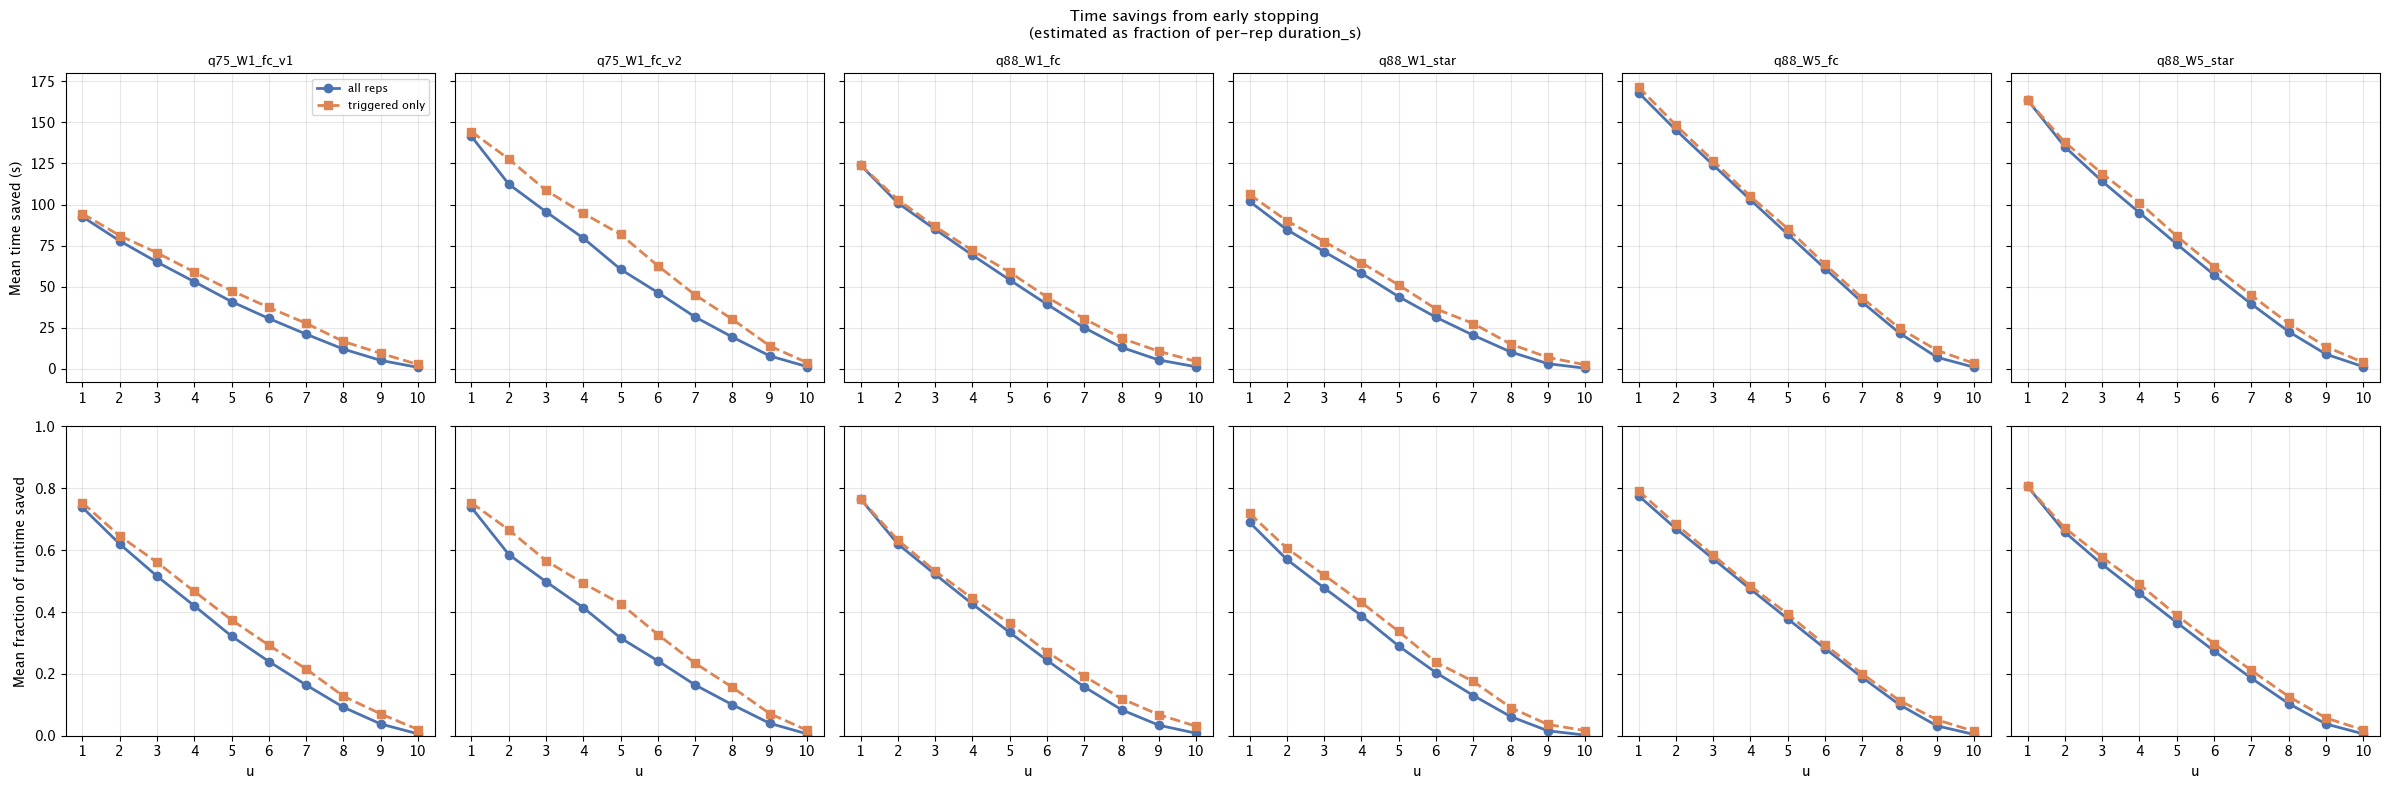
\includegraphics[width=0.75\linewidth]{figures/time_savings.png}
    \caption[Runtime saved by early stopping threshold]{Mean fraction of runtime saved by early stopping as a function of
    the threshold $u$. Solid line: all repetitions. Dashed line: only
    repetitions that triggered stopping. At $u = 3$ the saving is roughly
    $50\,\%$ per repetition.}
    \label{fig:time_savings}
\end{figure}

\paragraph{Output structure (fix, full \arguephase{}/\updatephase{}).}
The structured output is the measurement apparatus, not engineering taste.
Private reasoning and confidence versus the public message enable the
public/private dissociation; the \arguephase{} fields structure the deliberation
(the influence graph for dominance detection is built from vote adoptions, not the
draft text; \autoref{sec:method}); and the vote-stability rule separates argumentation
from belief update so they can be measured independently. Structured outputs are
the norm in serious MAD work \citep{liang2024encouraging, he2025dimo}.

\paragraph{Cooperativeness (fix, cooperative).}
\citet{liang2024encouraging} identify the operational sweet spot: a modest level
of tit-for-tat is required, with pure cooperation collapsing into
Degeneration-of-Thought and pure adversarial framing preventing convergence. Our
defense/challenge/question scaffold implements modest tit-for-tat while \updatephase{} phase
belief update leaves room for convergence.

\paragraph{Synchrony (fix, parallel-synchronous).}
\citet{du2024improving} establish synchronous simultaneous-talk as the canonical
MAD protocol, also adopted by \citet{liu2024groupdebate}. Synchronous execution
with randomised peer-message order also removes agent-order position effects that
would otherwise confound dominance detection.

\paragraph{Model selection (fix, homogeneous mid-tier).}
We fix a single homogeneous model, \texttt{mistral-medium-instruct}, to isolate topology
and memory effects from capability-asymmetry effects: \citet{wynn2025talk} document
that models shift from correct to incorrect answers under peer pressure, producing
dominance-like dynamics attributable to conformity. A homogeneous baseline ensures
any observed dominance is structural rather than capability-driven; heterogeneous
setups are reserved as an ablation. This choice is further supported by evidence
that mixed-model teams within the same capability tier do not systematically
outperform the best homogeneous member and exhibit comparable modal sycophancy
rates, suggesting heterogeneity alone does not dissolve the dynamics under study
\citep{bertalanic2026costofconsensus}.

\paragraph{Sampling temperature (fix at $0.7$, reasoning disabled).}
Deterministic decoding collapses MAD into voting among identical samples, and
\citet{zhu2026demystifying} show the homogeneous deterministic case cannot improve
over a single agent. We use temperature $0.7$ with reasoning disabled to obtain
diverse yet focused outputs without chain-of-thought token overhead. An ablation
comparing $T = 0.4$ against $T = 0.7$ in a comparable debate protocol found that
the lower temperature increased the modal sycophancy rate by $6.2$ percentage
points \citep{bertalanic2026costofconsensus}, providing external support for
the higher-temperature choice.

\paragraph{Tool access (defer).}
For GPQA-Diamond, tools would push single-agent accuracy toward the ceiling and
remove dynamical headroom, introduce non-reproducibility through web search, and
violate the Google-proof design rationale of \citet{rein2024gpqa}.

\paragraph{Compute budget.}
Reliable motif detection requires $R = 30$--$50$ repetitions per configuration:
bistability needs enough samples to surface both attractor basins, limit cycles
enough trajectories to confirm period-$\geq 2$ structure, and dominance
estimators statistical power. At $\approx 25$\,s per repetition, the naive cost of
the full grid on all 198 GPQA-Diamond tasks would be $198 \times 6 \times R \times
25$\,s, i.e.\ $\approx 248$\,h ($\approx 10.3$ days) at $R = 30$ and $\approx 413$\,h
($\approx 17.2$ days) at $R = 50$. The two-phase difficulty-based procedure of
\autoref{sec:setup:design} reduces this to $\approx 29$\,h by running the full
grid only on promoted Tier-3 tasks, while the screening pass still yields
prevalence estimates across the broader task set.

\newpage

\section{Electronic appendix}
\label{el_app}
The complete source code, including all scripts required to reproduce the figures and results, is publicly available in the following GitHub repository: 

\url{https://github.com/echtermeyer/LLM-Based-MAS}

\newpage

% ------------------------------------------------------------------------------
% BACK-MATTER LISTS (figures, tables, prompts) ---------------------------------
% ------------------------------------------------------------------------------
\phantomsection
\addcontentsline{toc}{section}{List of Figures}
\listoffigures
\newpage
\phantomsection
\addcontentsline{toc}{section}{List of Tables}
\listoftables
\newpage
\phantomsection
\addcontentsline{toc}{section}{List of Prompts}
\listof{prompt}{List of Prompts}
\newpage
    
% ------------------------------------------------------------------------------
% BIBLIOGRAPHY -----------------------------------------------------------------
% ------------------------------------------------------------------------------

\RaggedRight
\bibliography{bibliography}
\bibliographystyle{dcu}
\newpage

% ------------------------------------------------------------------------------
% DECLARATION OF AUTHORSHIP-----------------------------------------------------
% ------------------------------------------------------------------------------

\Large
\noindent
\textbf{Declaration of authorship} 
\vspace{0.3cm}
\noindent
\normalsize

I hereby declare that the report submitted is my own unaided work. All direct 
or indirect sources used are acknowledged as references. I am aware that the 
Thesis in digital form can be examined for the use of unauthorized aid and in 
order to determine whether the report as a whole or parts incorporated in it may 
be deemed as plagiarism. For the comparison of my work with existing sources I 
agree that it shall be entered in a database where it shall also remain after 
examination, to enable comparison with future Theses submitted. Further rights 
of reproduction and usage, however, are not granted here. This paper was not 
previously presented to another examination board and has not been published.

\vspace{0.7cm}
\Large
\noindent
\textbf{AI Tools}
\vspace{0.3cm}
\noindent
\normalsize

I hereby confirm that I have written all parts of this work myself. The following AI tools were used during the creation of this thesis and the presentations. All AI-generated suggestions and outputs were critically reviewed, tested where applicable, and independently revised by me. No AI tool was used for the main analysis or interpretation of experimental results.

\vspace{0.3cm}

\begin{itemize}
    \item \textbf{GitHub Copilot} (Inline Completion): Used for inline code completion suggestions during development. All outputs were reviewed and modified as appropriate.
    \item \textbf{Anthropic Claude Sonnet 5} (AI as Tutor): Used to explore and understand core concepts in complex-systems theory and multi-agent debate.
    \item \textbf{Anthropic Claude Opus 5} (Performance and Resource Optimization): Used to parallelize the evaluation pipeline for the experiments described in \autoref{sec:exp} and reported in \autoref{sec:results}. The generated code was reviewed and tested carefully.
    \item \textbf{Anthropic Claude Opus 5} (Improve Writing Style, Paraphrasing and Reformulation): Used for proofreading, linguistic refinement, and paraphrasing. Suggestions were not adopted verbatim but were manually reviewed, adapted, and reformulated.
\end{itemize}

All AI outputs and suggestions were independently evaluated and selectively adopted after critical review.

\vspace{0.8cm}
München, 30.09.2026 \\

\vspace{1cm}

\noindent\rule{0.5\textwidth}{0.4pt} \\

\myname

% ------------------------------------------------------------------------------

\end{document}
